% Optimal Athletic Programming in Triathlon -- defence slides.
%
% Two builds from this one source:
%   pdflatex presentation.tex
%       -> presentation.pdf: the slides, exactly as projected
%   xelatex -jobname=presentation-notes "\def\shownotes{}% Optimal Athletic Programming in Triathlon -- defence slides.
%
% Two builds from this one source:
%   pdflatex presentation.tex
%       -> presentation.pdf: the slides, exactly as projected
%   xelatex -jobname=presentation-notes "\def\shownotes{}% Optimal Athletic Programming in Triathlon -- defence slides.
%
% Two builds from this one source:
%   pdflatex presentation.tex
%       -> presentation.pdf: the slides, exactly as projected
%   xelatex -jobname=presentation-notes "\def\shownotes{}% Optimal Athletic Programming in Triathlon -- defence slides.
%
% Two builds from this one source:
%   pdflatex presentation.tex
%       -> presentation.pdf: the slides, exactly as projected
%   xelatex -jobname=presentation-notes "\def\shownotes{}\input{presentation}"
%       -> presentation-notes.pdf: the same slides with the Greek speaker notes
%          (xelatex, because the notes are in Greek and need a Unicode font)
%
% presentation-notes.pdf is a private rehearsal aid and is NOT committed.
%
% Design rule for this deck: the slide is the evidence, the speaker is the
% argument. Anything that is a sentence rather than a number, a name or a
% figure belongs in \note{}, not on screen.

\documentclass[10pt,aspectratio=169]{beamer}

\usetheme{Madrid}
\usecolortheme{seahorse}
\setbeamertemplate{navigation symbols}{}
\usepackage{amsmath,amssymb}
\usepackage{graphicx}
\usepackage{booktabs}

\ifdefined\shownotes
  \setbeameroption{show notes}
  \usepackage{fontspec}
  % Any installed font with Greek coverage; Helvetica ships with macOS.
  % Override on another machine, e.g. \def\notesfont{DejaVu Sans}
  \providecommand{\notesfont}{Helvetica}
  \newfontfamily\gr{\notesfont}
\else
  \providecommand{\gr}{}
\fi

\graphicspath{{../results/figures/}}

\definecolor{accent}{RGB}{30,60,140}
\setbeamercolor{frametitle}{fg=white,bg=accent}
\setbeamercolor{title}{fg=white,bg=accent}

% one-line takeaway strip under a figure
\newcommand{\takeaway}[1]{\vspace{2pt}\begin{center}\small\textbf{#1}\end{center}}

\title[Triathlon Optimization]{Optimal Resource Allocation and Scheduling\\
       of Athletic Activities, with an Application to Triathlon}
\subtitle{\normalsize Linear and 0--1 Integer Programming models for training
          load, race calendar and race pacing}
\author[E. Vichos]{Emmanouil Vichos (AM 1100830)}
\institute[UPatras]{Linear and Combinatorial Optimization --- University of Patras\\
                    Supervisor: Prof.\ S.\ Daskalaki}
\date{\today}

\begin{document}

\begin{frame}
\titlepage
\end{frame}

\note{\gr Καλημέρα σας. Η εργασία μου εφαρμόζει γραμμικό και ακέραιο
προγραμματισμό στο τρίαθλο --- και μάλιστα όχι σε πλασματικά δεδομένα: σε
δεκαπέντε μήνες δικής μου προπόνησης και σε τρεις αγώνες που πραγματικά έτρεξα.
Τρεις αποφάσεις, τρία μοντέλα, μία αλυσίδα.}

% ---------------------------------------------------------------- overview
\begin{frame}{Three decisions, one athlete}
\begin{enumerate}\itemsep8pt
  \item<1-> \textbf{How to train} --- hours per sport, per intensity, per week
  \item<2-> \textbf{Which races to enter} --- a season under money and recovery limits
  \item<3-> \textbf{How to race} --- spend a finite energy reserve over three legs
\end{enumerate}
\vspace{14pt}
\onslide<4->{
\begin{center}\large
\textbf{Model 1 (LP)} $\;\rightarrow\;$ \textbf{Model 2 (0--1 MIP)} $\;\rightarrow\;$ \textbf{Model 3 (LP)}\\[2pt]
\small training load \hfill race calendar \hfill pacing strategy
\end{center}}
\end{frame}

\note{\gr Οι τρεις αποφάσεις δεν είναι ανεξάρτητες, και αυτό ακριβώς είναι το
νόημα της εργασίας. Η φυσική κατάσταση χτίζεται αργά ενώ η κόπωση γρήγορα, οπότε
η προπόνηση είναι ένα δυναμικό trade-off σε ορίζοντα 12 έως 20 εβδομάδων.

Η κατάσταση φόρμας που βγάζει το Μοντέλο 1 κάνει μετά δύο πράγματα: καθορίζει σε
ποιους αγώνες είμαι έτοιμος να κατέβω, και ορίζει το ενεργειακό budget που έχω
διαθέσιμο την ημέρα του αγώνα. Άρα τα βέλη είναι πραγματικές συζεύξεις, όχι
αφηγηματικό στολίδι.}

% ---------------------------------------------------------------- data
\begin{frame}{Real data: 15 months of my own training}
\begin{columns}
\column{.55\textwidth}
\begin{itemize}\itemsep6pt
  \item Strava export: \textbf{598 activities}, 574 usable
  \item Banister training impulse per activity
  \item Fitness CTL ($\tau{=}42$d), fatigue ATL ($\tau{=}7$d)
  \item Today: CTL $78.1$, ATL $91.5$, \textbf{TSB $-13.4$}
\end{itemize}
\column{.42\textwidth}
\centering\small
\begin{tabular}{lrrr}
\toprule
$r_{db}$/h & easy & mod & hard\\
\midrule
swim & 43.5 & $94.1^\ast$ & $136.6^\ast$\\
bike & 68.3 & 86.9 & $142.7^\ast$\\
run  & 81.6 & 102.8 & $166.0^\ast$\\
\bottomrule
\end{tabular}

\vspace{4pt}
{\scriptsize load rate per hour \quad $^\ast$theoretical (sparse data)}
\end{columns}
\end{frame}

\note{\gr Το export είναι 598 δραστηριότητες από τον Οκτώβριο του 2023 μέχρι τον
Ιούνιο του 2026· οι 574 επιβιώνουν του καθαρισμού. Κάθε μία παίρνει ένα Banister
training impulse --- διάρκεια επί το heart rate reserve επί έναν εκθετικό
συντελεστή. Δύο εκθετικές εξομαλύνσεις αυτής της σειράς δίνουν το CTL με σταθερά
42 ημερών και το ATL με σταθερά 7 ημερών· η διαφορά τους είναι το TSB, η φόρμα.
Αυτή τη στιγμή είμαι σε καλή κατάσταση αλλά κουρασμένος: μείον 13,4.

Ο πίνακας δεξιά είναι η γέφυρα από τα δεδομένα στο μοντέλο: ρυθμός φόρτισης ανά
ώρα, ανά άθλημα, ανά ζώνη έντασης. Οι ζώνες κόβονται ως προς threshold καρδιακό
παλμό ξεχωριστά για κάθε άθλημα --- 173 στο τρέξιμο, 166 στο ποδήλατο, 164 στο
κολύμπι --- γιατί ο ίδιος παλμός δεν σημαίνει το ίδιο πράγμα μέσα στο νερό και
πάνω στο ποδήλατο.

Τα κελιά με αστερίσκο είναι εκεί που έχω λίγα δεδομένα και χρειάστηκε να τα
ορίσω από τη βιβλιογραφία. Τα επισημαίνω επειδή είναι τα πιο αδύναμα inputs του
Μοντέλου 1.}

% ---------------------------------------------------------------- model 1
\begin{frame}{Model 1 --- training-load allocation (LP)}
\textbf{Variables} \quad hours $h_{dbw} \ge 0$: 3 sports $\times$ 3 buckets
$\times$ 16 weeks $= 144$
\vspace{6pt}

\textbf{Banister dynamics, as linear equalities}
\[
L_w = \sum_{d,b} r_{db} h_{dbw}, \qquad
\text{CTL}_w = \lambda_c \text{CTL}_{w-1} + (1{-}\lambda_c)\tfrac{L_w}{7}, \qquad
\text{ATL}_w = \lambda_a \text{ATL}_{w-1} + (1{-}\lambda_a)\tfrac{L_w}{7}
\]

\textbf{Objective} \quad
$\max\; p_T = k_1 \text{CTL}_T - k_2 \text{ATL}_T$
\vspace{6pt}

\textbf{Constraints} \quad weekly hour ceilings $\cdot$ per-sport min/max $\cdot$
80/20 polarization $\cdot$ $\text{ATL} \le 110$ $\cdot$ ramp $\le +10\%$/week
$\cdot$ taper caps
\end{frame}

\note{\gr Εκατόν σαράντα τέσσερις μεταβλητές, όλες συνεχείς και μη αρνητικές.

Το σημαντικό σημείο μοντελοποίησης είναι η δεύτερη γραμμή. Οι αναδρομές του
Banister είναι εκθετικές εξομαλύνσεις, και η εκθετική εξομάλυνση είναι γραμμική
ως προς το φορτίο. Άρα η φυσιολογία μπαίνει στο LP ως ακριβείς ισότητες --- δεν
προσεγγίζω κάποιο μη γραμμικό σύστημα, η δυναμική είναι πράγματι γραμμική ως
προς τις μεταβλητές απόφασής μου.

Για την αντικειμενική συνάρτηση: το προφανές θα ήταν να μεγιστοποιήσω τη φόρμα,
το TSB, δηλαδή CTL μείον ATL. Αυτό όμως είναι εκφυλισμένο --- το βέλτιστο είναι
να μην κάνω τίποτα, γιατί η ξεκούραση μηδενίζει το ATL. Γι' αυτό τα σταθμίζω
χωριστά, k1 επί CTL μείον k2 επί ATL, με το k2 μεγαλύτερο από το k1, που
μεταφράζεται ότι η κόπωση βλάπτει την ημέρα του αγώνα περισσότερο απ' όσο
βοηθάει η φόρμα. Θα επανέλθω στο αν αυτά τα βάρη στέκουν.

Οι περιορισμοί είναι η προπονητική πρακτική διατυπωμένη τυπικά: ταβάνι
εβδομαδιαίων ωρών, κατώφλι και πλαφόν ανά άθλημα ώστε να μη μηδενιστεί το
κολύμπι, ο κανόνας πόλωσης 80/20, ένα σκληρό ταβάνι κόπωσης, ο κανόνας αύξησης
10\% την εβδομάδα, και υποχρεωτικό taper στις δύο τελευταίες εβδομάδες.}

\begin{frame}{Model 1 --- the optimizer discovers periodization}
\centering
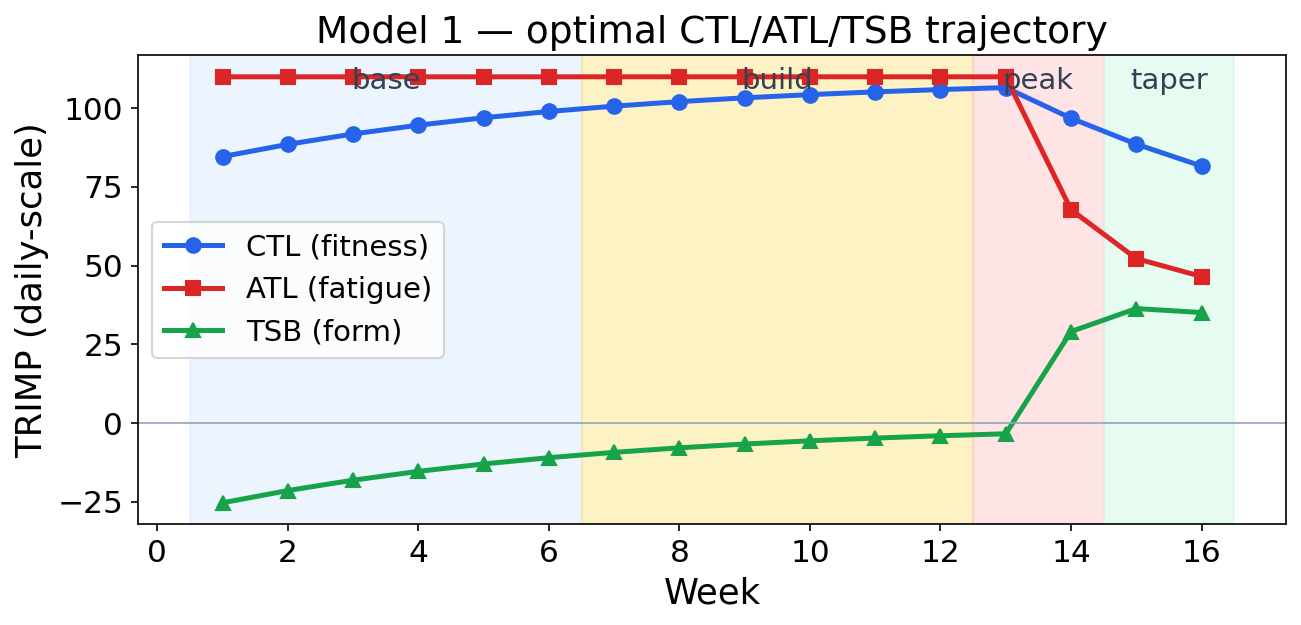
\includegraphics[width=.72\textwidth]{model1_trajectory.png}
\takeaway{Nobody told it to periodize. Week 14 tapers by choice.}
\end{frame}

\note{\gr Αυτό είναι το αγαπημένο μου αποτέλεσμα σε όλη την εργασία. Πουθενά στο
μοντέλο δεν γράφει «κάνε περιοδικότητα». Οι περιορισμοί είναι τοπικοί --- ένας
ρυθμός αύξησης, ένα ταβάνι, ένα κατώφλι --- και ο optimizer παράγει μόνος του
τον κλασικό μακρόκυκλο: κυλάει πάνω στο ταβάνι κόπωσης για δεκατρείς εβδομάδες,
ανεβάζοντας το CTL από 78 στο 107, και μετά κάνει taper.

Και προσέξτε την εβδομάδα 14. Μόνο οι εβδομάδες 15 και 16 είναι αναγκασμένες να
κάνουν taper. Η 14 κάνει taper επειδή το LP υπολογίζει ότι η κόπωση την ημέρα
του αγώνα κοστίζει περισσότερο απ' ό,τι αξίζει η φόρμα που θα αγόραζαν εκείνες
οι ώρες. Δηλαδή το μοντέλο ξαναβγάζει μόνο του προπονητική γνώση, από καθαρή
αριθμητική. Η φόρμα την ημέρα του αγώνα βγαίνει συν 35.}

\begin{frame}{Model 1 --- duality in action}
\begin{columns}
\column{.5\textwidth}
\centering
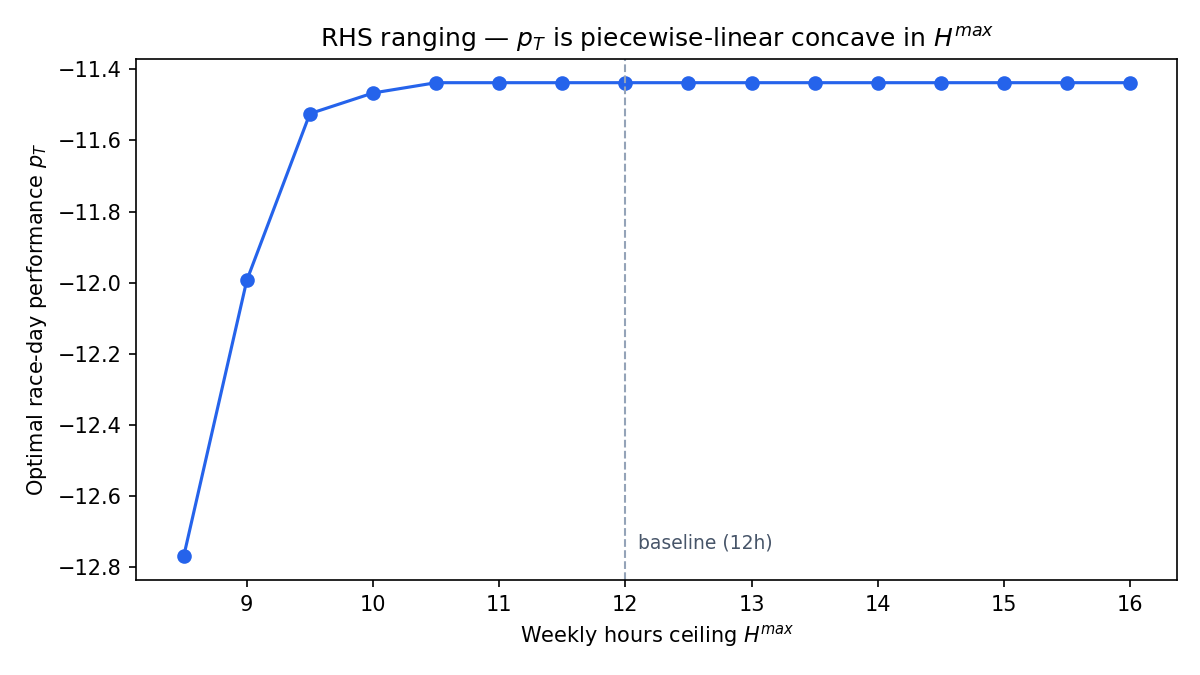
\includegraphics[width=\textwidth]{model1_rhs_ranging.png}
\column{.48\textwidth}
\textbf{RHS ranging:} the hours ceiling, 8--16 h
\begin{itemize}\itemsep6pt
  \item piecewise-linear, concave
  \item slopes $1.55 \to 0.94 \to 0.12 \to 0$
  \item flat above \textbf{10.5 h/week}
\end{itemize}
\vspace{10pt}
\begin{center}
\emph{Recovery capacity, not free time,\\ is what limits this athlete.}
\end{center}
\end{columns}
\end{frame}

\note{\gr Εδώ είναι η ανάλυση ευαισθησίας του μαθήματος, εφαρμοσμένη σε ένα
ερώτημα που με αφορά πραγματικά: αξίζει να ψάξω να βρω κι άλλες ώρες για
προπόνηση;

Μεταβάλλω το δεξί μέλος του περιορισμού των εβδομαδιαίων ωρών από 8 έως 16 και
σχεδιάζω τη βέλτιστη τιμή. Βγαίνει το σχήμα που προβλέπει η θεωρία: κατά
τμήματα γραμμική και κοίλη, επειδή κάθε σημείο καμπής είναι μια αλλαγή βάσης. Οι
κλίσεις είναι οι σκιώδεις τιμές: 1,55 μετά 0,94 μετά 0,12 και μετά μηδέν.

Η απάντηση βρίσκεται στις 10,5 ώρες. Από εκεί και πάνω η σκιώδης τιμή είναι
μηδέν: οι επιπλέον ώρες δεν αξίζουν τίποτα, γιατί το ταβάνι του ATL δεσμεύει
πριν προλάβει να δεσμεύσει το ταβάνι του χρόνου. Το στενό μου σημείο δεν είναι
το πρόγραμμά μου, είναι το πόσο γρήγορα ανακάμπτω.

Να αναφέρω και μία ακόμα δυϊκή τιμή: οι μεγαλύτερες σκιώδεις τιμές όλου του
μοντέλου είναι στους περιορισμούς ελάχιστης προπόνησης της εβδομάδας του αγώνα
--- μείον 12,9 ανά αναγκαστική ώρα τρεξίματος στην εβδομάδα 16. Το μοντέλο θέλει
απόλυτη ξεκούραση κι εγώ το υποχρεώνω να προπονηθεί.}

% ---------------------------------------------------------------- model 2
\begin{frame}{Model 2 --- race-calendar selection (0--1 MIP)}
\textbf{17 candidate races}, binary $x_i$
\[
\max \sum_i \underbrace{q_i(\alpha\,\text{pts}_i + \beta\,\text{strat}_i
+ \gamma\,\text{enj}_i + \varphi\,\text{fit}_i)}_{\text{weather-risk-adjusted value}} x_i
\]
\begin{itemize}\itemsep6pt
  \item \textbf{two knapsacks:} $\le 2500$ EUR, $\le 12$ vacation days
  \item \textbf{recovery spacing:} $x_i + x_j \le 1$; $\le 2$ races/month; $\ge 1$ A-race
  \item \textbf{readiness gate from Model 1:} projected CTL must reach the class
\end{itemize}
\end{frame}

\note{\gr Δεκαεπτά υποψήφιοι αγώνες --- ελληνικοί, ευρωπαϊκοί και δύο
υπερατλαντικοί --- ο καθένας με μία δυαδική μεταβλητή.

Η αξία κάθε αγώνα είναι τέσσερα σταθμισμένα συστατικά: βαθμοί παγκόσμιας
κατάταξης, στρατηγική σημασία, πόσο θα τον ευχαριστηθώ, και πόσο μου ταιριάζει η
διαδρομή. Το τελευταίο δεν είναι αίσθηση: υπολογίζεται από αντικειμενικά
δεδομένα διαδρομής, υψομετρική διαφορά ανά χιλιόμετρο σε σχέση με τη δική μου
προτίμηση σε επίπεδες διαδρομές. Και όλο αυτό πολλαπλασιάζεται με το q, έναν
συντελεστή καιρικού ρίσκου, ώστε ένας αγώνας με ιστορικό ακυρώσεων ή ακραίας
ζέστης να προεξοφλείται.

Τρεις οικογένειες περιορισμών. Δύο σακίδια --- χρήματα και ημέρες άδειας ---
που κάνουν το πρόβλημα δισδιάστατο knapsack. Ανά ζεύγος περιορισμοί αποθεραπείας,
μία, δύο ή τέσσερις εβδομάδες ανάλογα με την κατηγορία απόστασης, γραμμένοι με
τον τυπικό περιορισμό σύγκρουσης: x-i συν x-j το πολύ ένα. Και η πύλη
ετοιμότητας: το προβλεπόμενο CTL από το Μοντέλο 1 πρέπει να φτάνει την απαίτηση
της κατηγορίας --- εδώ ακριβώς μπαίνει φυσικά το Μοντέλο 1 μέσα στο Μοντέλο 2.
Αυτή η πύλη αποκλείει ένα 70.3 υψηλής αξίας στην αρχή της σεζόν: απλούστατα δεν
θα προλάβω να είμαι έτοιμος.}

\begin{frame}{Model 2 --- optimal season}
\centering
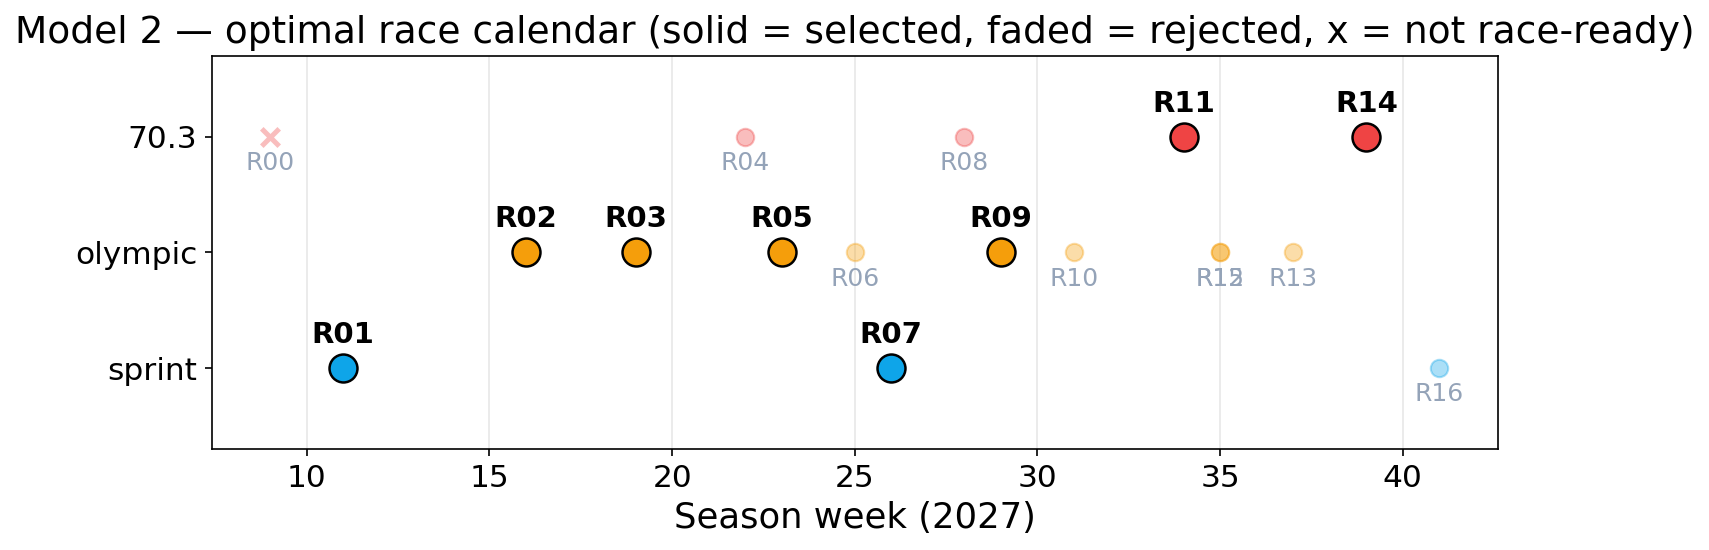
\includegraphics[width=.78\textwidth]{model2_calendar.png}
\takeaway{8 of 17 races $\cdot$ value 571.7 $\cdot$ 2250/2500 EUR $\cdot$ 11/12 days}
\end{frame}

\note{\gr Οκτώ αγώνες από τους δεκαεπτά, συνολική αξία 571,7. Ξοδεύει 2250 από τα
2500 ευρώ και 11 από τις 12 ημέρες άδειας --- άρα και τα δύο σακίδια είναι σχεδόν
γεμάτα, αλλά κανένα δεν δεσμεύει ακριβώς, κάτι που θα έχει σημασία σε δύο
διαφάνειες.

Η ενδιαφέρουσα απόφαση είναι το φθινόπωρο. Το Πανελλήνιο Πρωτάθλημα και το 70.3
της περιοχής μου είναι αρκετά κοντά ώστε ο περιορισμός αποθεραπείας να απαγορεύει
και τα δύο. Ο optimizer κρατάει το 70.3.

Τα «χι» είναι αγώνες για τους οποίους δεν είμαι αρκετά έτοιμος· οι ξεθωριασμένοι
κύκλοι είναι αγώνες που θα μπορούσε να πληρώσει αλλά επέλεξε να μην τους
αγοράσει.}

\begin{frame}{Model 2 --- why Branch \& Bound is needed}
\begin{columns}
\column{.52\textwidth}
\centering
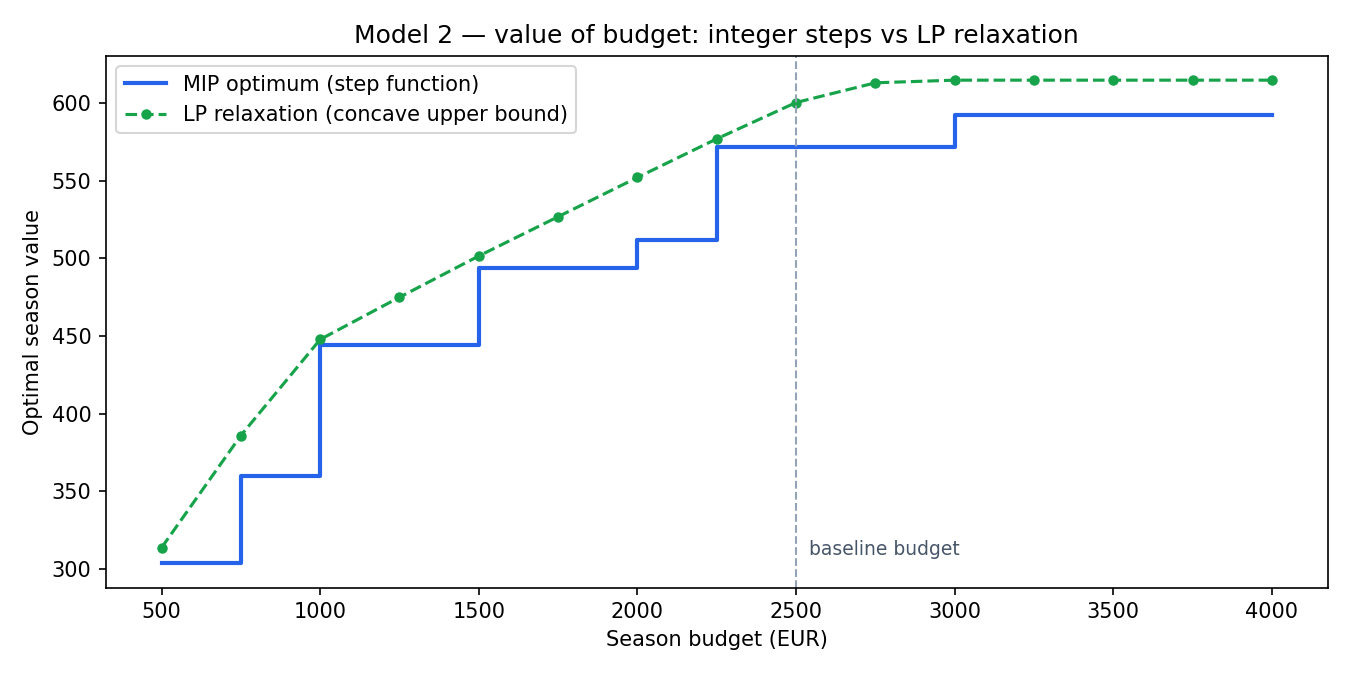
\includegraphics[width=\textwidth]{model2_budget_sweep.png}
\column{.46\textwidth}
\begin{itemize}\itemsep8pt
  \item LP $600.5$ vs.\ MIP $571.7$:\\ \textbf{integrality gap 5.0\%}
  \item 8 fractional variables; the champs/70.3 conflict splits \textbf{0.5/0.5}
  \item \textbf{clique cuts} (Bron--Kerbosch): $600.5 \to 591.0$,\\
        gap \textbf{5.04\% $\to$ 3.38\%}
\end{itemize}
\end{columns}
\end{frame}

\note{\gr Γιατί δεν λύνω απλώς τη γραμμική χαλάρωση και στρογγυλοποιώ; Επειδή η
χαλάρωση δίνει 600,5 έναντι πραγματικού βέλτιστου 571,7 --- κενό ακεραιότητας 5
τοις εκατό --- και οκτώ μεταβλητές βγαίνουν κλασματικές. Η σύγκρουση Πρωτάθλημα
εναντίον 70.3 που μόλις περιέγραψα σπάει ακριβώς μισό-μισό: η χαλάρωση παίρνει
μισό από κάθε αγώνα, που δεν σημαίνει τίποτα. Χρειάζεται Branch and Bound.

Το σχήμα είναι η αξία του χρήματος. Το βέλτιστο του MIP είναι κλιμακωτή
συνάρτηση --- οι αγώνες κοστίζουν όσο κοστίζουν, οπότε τα επιπλέον ευρώ δεν
κάνουν τίποτα μέχρι να φτάσουν να πληρώσουν άλλη μία συμμετοχή --- και βρίσκεται
κάτω από την κοίλη καμπύλη της χαλάρωσης. Πάνω από τα 3000 ευρώ τα σκαλοπάτια
σταματούν, γιατί ο δεσμευτικός πόρος αλλάζει από χρήματα σε ημέρες άδειας.

Για τα cutting planes: φτιάχνω τον γράφο συγκρούσεων των περιορισμών αποθεραπείας
και τρέχω Bron--Kerbosch για να βρω τις μέγιστες κλίκες του. Κάθε κλίκα μεγέθους
τρία ή παραπάνω δίνει μια έγκυρη ανισότητα, άθροισμα των x της κλίκας το πολύ
ένα, που κυριαρχεί των ανά ζεύγος περιορισμών. Τέσσερις τέτοιες τομές σφίγγουν τη
χαλάρωση από 600,5 σε 591, κλείνοντας το ένα τρίτο του κενού, και δεν αποκόπτουν
κανένα ακέραιο σημείο --- το βέλτιστο μένει αμετάβλητο.}

\begin{frame}{Model 2 --- the dual problem}
\[
\kappa_i y_\mathcal{B} + \delta_i y_\mathcal{D} + y_{\text{month}(i)}
+ \sum_{j} y_{ij} - [i \in A] y_A \;\ge\; v_i
\]
\begin{center}\small
\emph{a race enters only if its value covers the shadow cost of what it consumes}
\end{center}
\vspace{4pt}
\begin{center}\small
\begin{tabular}{llr}
\toprule
Dual & Meaning & Price\\
\midrule
$y_{13,14}$ & Champs vs.\ Costa Navarino conflict & \textbf{56.40}\\
$y_{06,07}$ & Hamburg vs.\ Thessaloniki conflict & 31.67\\
$y_\mathcal{B}$ & one extra euro & 0.094\\
$y_\mathcal{D}$ & one extra vacation day & $\approx 0$\\
\bottomrule
\end{tabular}
\end{center}
\takeaway{The scarce resource is calendar space --- not money.}
\end{frame}

\note{\gr Η γραμμική χαλάρωση είναι ήδη σε τυπική μορφή, max c-ανάστροφο-x υπό Ax
μικρότερο ή ίσο του b με x μη αρνητικό, οπότε το δυϊκό είναι το σχολικό: min
b-ανάστροφο-y με A-ανάστροφο-y μεγαλύτερο ή ίσο του c. Γράφοντας μία δυϊκή γραμμή
παίρνω την ανισότητα της διαφάνειας, και έχει καθαρή ανάγνωση: ένας αγώνας μπαίνει
στο ημερολόγιο μόνο αν η αξία του καλύπτει το σκιώδες κόστος όλων όσων καταναλώνει
--- budget, ημέρες άδειας, τη θέση του μήνα του, και κάθε σύγκρουση στην οποία
συμμετέχει.

Τώρα διαβάστε τις τιμές. Ένα ευρώ αξίζει 0,094. Μία ημέρα άδειας ουσιαστικά
μηδέν. Αλλά η σύγκρουση αποθεραπείας ανάμεσα στο Πρωτάθλημα και στην Costa
Navarino τιμολογείται στο 56,4 --- τρεις τάξεις μεγέθους πάνω από το ευρώ.

Άρα η διαίσθηση με την οποία ξεκίνησα ήταν λάθος. Υπέθετα ότι ο περιορισμός ήταν
τα χρήματα. Το δυϊκό λέει ότι ο σπάνιος πόρος είναι ο χώρος στο ημερολόγιο: οι
εβδομάδες αποθεραπείας μεταξύ αγώνων. Πρακτικά, το να διαπραγματευτώ ημερομηνίες
αξίζει πολύ περισσότερο από το να βρω χορηγία.}

\begin{frame}{Model 2 --- network-flow extension}
Drop the knapsacks and the monthly cap $\Rightarrow$ only recovery spacing remains:
\begin{center}
\textbf{feasible calendars $=$ paths in a DAG}
\end{center}
\vspace{6pt}
Three methods, identical answer $z = 639.4$:
\begin{enumerate}\itemsep4pt
  \item dynamic programming --- longest path in topological order
  \item \textbf{flow LP, continuous variables --- integral anyway}
  \item restricted 0--1 MIP
\end{enumerate}
\takeaway{Totally unimodular. The knapsacks are what break the structure.}
\end{frame}

\note{\gr Αυτή η διαφάνεια συνδέει την εργασία με το κομμάτι των δικτύων της ύλης.

Αν αφαιρέσω τα δύο σακίδια και το μηνιαίο πλαφόν, και κρατήσω μόνο την
αποθεραπεία, το πρόβλημα αλλάζει τελείως χαρακτήρα. Βάζω τους αγώνες ως κόμβους
σε σειρά εβδομάδας και τραβάω ακμή από τον i στον j όταν το κενό είναι
τουλάχιστον όσο η αποθεραπεία που απαιτεί ο i. Τότε ένα εφικτό ημερολόγιο είναι
ακριβώς μια διαδρομή σε αυτό το κατευθυνόμενο άκυκλο γράφημα, και το καλύτερο
ημερολόγιο είναι η μακρύτερη διαδρομή.

Το έλυσα με τρεις τρόπους και πήρα 639,4 και τις τρεις φορές. Ο μεσαίος είναι το
θεωρητικό σημείο: το έλυσα ως LP ροής με συνεχείς μεταβλητές, χωρίς κανέναν
περιορισμό ακεραιότητας, και η λύση βγήκε ακέραια από μόνη της. Αυτό είναι ολική
μονοπαραγοντικότητα --- ο πίνακας πρόσπτωσης κόμβων-ακμών είναι TU, άρα κάθε
βασική εφικτή λύση είναι ακέραια και κάθε βάση αντιστοιχεί σε ένα συνδετικό
δέντρο. Αυτή ακριβώς είναι η δομή που εκμεταλλεύεται ο Network Simplex. Δεκαοκτώ
κόμβοι, 136 ακμές.

Και αυτό λέει κάτι για το πλήρες μοντέλο: είναι οι περιορισμοί σακιδίου, το
budget και οι ημέρες άδειας, που καταστρέφουν τη δομή δικτύου και επιβάλλουν
Branch and Bound. Χωρίς αυτούς, δεν χρειάζεται καθόλου διακλάδωση.}

% ---------------------------------------------------------------- model 3
\begin{frame}{Model 3 --- race pacing (LP with linearization)}
\textbf{Variables} \quad minutes $t_{\ell z}$: 3 legs $\times$ 5 zones $= 15$
\vspace{4pt}

\textbf{Linearization} \quad within a zone, speed and energy rate are \emph{constants}
\[
\min \sum_{\ell,z} t_{\ell z} + T_1 + T_2
\quad \text{s.t.} \quad
\underbrace{\textstyle\sum_z s_{\ell z} t_{\ell z} \ge d_\ell}_{\text{distances}},\;
\underbrace{\textstyle\sum e_{\ell z} t_{\ell z} \le k_E \cdot \text{CTL}_T}_{\text{energy budget (Model 1)}},\;
\underbrace{\text{Z4+ caps}}_{\text{per leg}},\;
\underbrace{\varphi \cdot G}_{\text{bike} \to \text{run}}
\]
\vspace{-6pt}
\begin{center}\small
bike speed $\propto \phi(\gamma)\cdot(\text{power})^{1/3}$ \quad --- \quad
$\phi(\gamma)$ from the power balance, \textbf{derived, not fitted}
\end{center}
\end{frame}

\note{\gr Εδώ η φυσική είναι μη γραμμική: η σχέση ταχύτητας και ενεργειακού
κόστους είναι καμπύλη, όχι ευθεία. Το κόλπο είναι να διακριτοποιήσω την ένταση
στις πέντε προπονητικές ζώνες. Μέσα σε μια ζώνη, η ταχύτητα και ο ρυθμός
κατανάλωσης είναι σταθερές, άρα και η απόσταση και η ενέργεια γίνονται γραμμικές
ως προς τον χρόνο που ξοδεύω εκεί, και το πρόβλημα ξαναγίνεται LP. Δεκαπέντε
μεταβλητές. Αυτή είναι η κλασική κατά τμήματα γραμμική προσέγγιση του μαθήματος,
και οι ζώνες δεν είναι αυθαίρετες --- είναι οι ζώνες στις οποίες προπονούνται
πραγματικά οι αθλητές.

Δύο όροι αξίζουν κουβέντα. Η ταχύτητα στο ποδήλατο πάει με την κυβική ρίζα της
ισχύος, επειδή η αεροδυναμική αντίσταση πάει με την ταχύτητα στον κύβο --- αν
διπλασιάσεις την ισχύ σου δεν πλησιάζεις καν τον διπλασιασμό της ταχύτητας.

Και το φι του γάμμα είναι ο συντελεστής κλίσης της διαδρομής. Μοντελοποιώ μια
διαδρομή που ανεβαίνει γάμμα μέτρα ανά χιλιόμετρο ως μισή ανηφόρα και μισή
κατηφόρα με σταθερή ισχύ, και παίρνω τον αρμονικό μέσο των δύο ταχυτήτων. Η
αεροδυναμική σταθερά προκύπτει αντίστροφα από τη δική μου ταχύτητα σε επίπεδη
διαδρομή, οπότε τίποτα μέσα στο φι δεν είναι προσαρμοσμένο σε αποτέλεσμα αγώνα.
Αυτό θα έχει σημασία στην επικύρωση, τρεις διαφάνειες πιο κάτω.

Ο τελευταίος όρος είναι η σύζευξη που κάνει το πρόβλημα τρίαθλο και όχι τρεις
ξεχωριστούς αγώνες: κάθε κιλοτζάουλ σκληρής δουλειάς στο ποδήλατο μειώνει το πόσο
μακριά μπορώ μετά να τρέξω.}

\begin{frame}{Model 3 --- ``steady bike, hard run,'' derived}
\centering
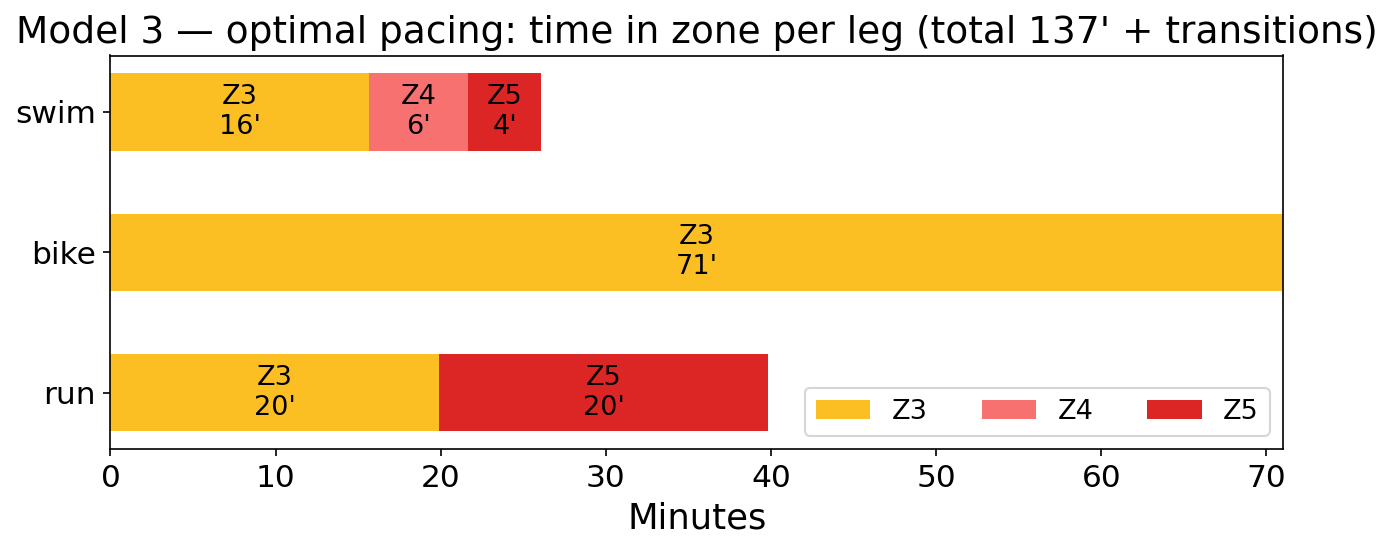
\includegraphics[width=.70\textwidth]{model3_pacing.png}
\takeaway{Bike entirely Z3. Energy budget exhausted \emph{exactly}: 9389 kJ.}
\end{frame}

\note{\gr Ολυμπιακή απόσταση σε 140,4 λεπτά, και το ενεργειακό budget εξαντλείται
ακριβώς --- 9389 κιλοτζάουλ διαθέσιμα, 9389 καταναλωμένα. Ο ενεργειακός
περιορισμός είναι δεσμευτικός, γι' αυτό και η δυϊκή του τιμή είναι το ενδιαφέρον
νούμερο της επόμενης διαφάνειας.

Η δομή της απάντησης είναι το προπονητικό κλισέ «σταθερό ποδήλατο, δυνατό
τρέξιμο», και το LP το βγάζει χωρίς να του το πει κανείς. Το ποδήλατο είναι
εξ ολοκλήρου στη ζώνη 3, τίποτα πιο σκληρό. Γιατί; Για δύο λόγους, και οι δύο
μέσα στο μοντέλο: η κυβική ρίζα σημαίνει ότι το σκληρό ποδήλατο αγοράζει ελάχιστη
ταχύτητα, και ο όρος σύζευξης σημαίνει ότι σου κοστίζει άμεσα απόσταση στο
τρέξιμο. Οπότε ο optimizer ξοδεύει την ένταση εκεί που η ένταση είναι φθηνή,
δηλαδή στο τρέξιμο.}

\begin{frame}{Model 3 --- what is a watt worth?}
\centering
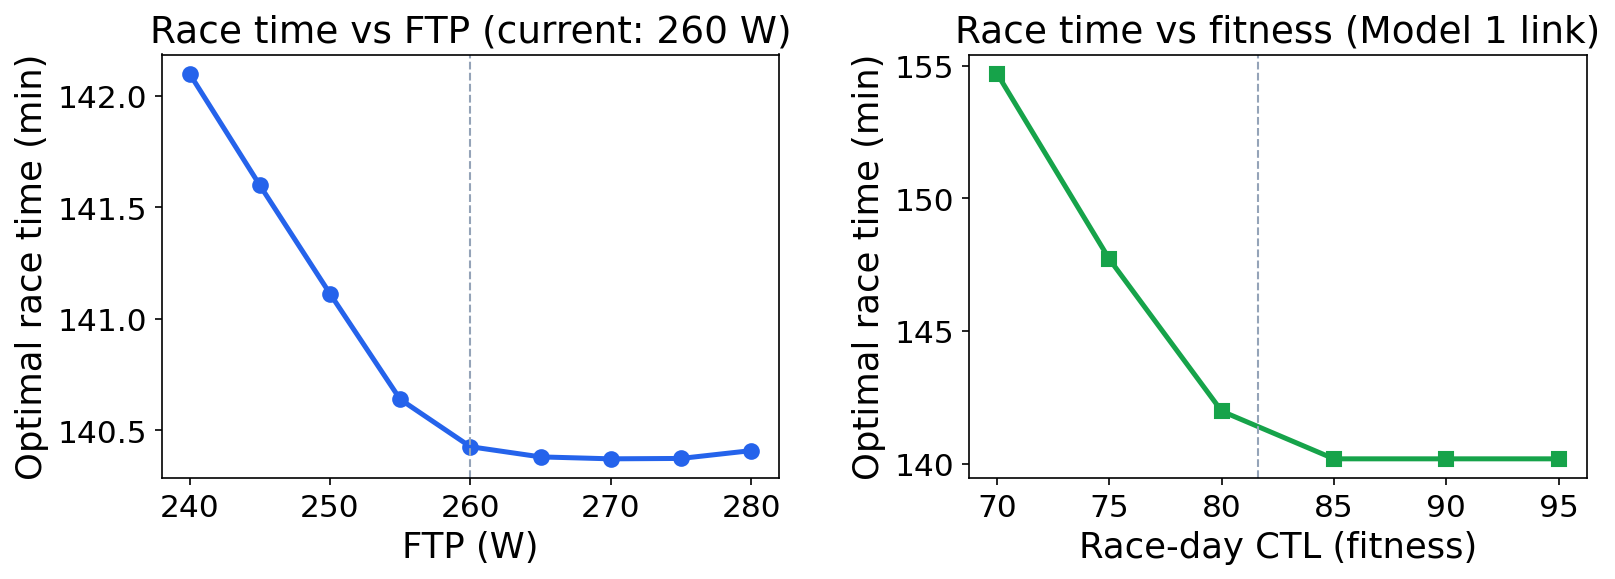
\includegraphics[width=.86\textwidth]{model3_sweeps.png}
\takeaway{$+1$ CTL $=$ 69--84 s. $+1$ W $\approx$ 6 s --- but only below 260 W.}
\end{frame}

\note{\gr Δύο σαρώσεις ευαισθησίας, και οι δύο απαντούν σε ερωτήματα που κάνει
ένας πραγματικός αθλητής.

Αριστερά: τι αξίζει ένα βατ; Κάτω από τα 260 βατ, κάθε επιπλέον βατ threshold
ισχύος αξίζει περίπου έξι δευτερόλεπτα. Πάνω από εκεί, η αξία καταρρέει στο μηδέν.
Αυτό δεν είναι σφάλμα --- είναι ο ενεργειακός περιορισμός. Με σταθερό απόθεμα
κιλοτζάουλ, δεν έχει νόημα να μπορείς να παράγεις περισσότερη ισχύ, γιατί δεν
μπορείς να την τροφοδοτήσεις. Το σκέλος του ποδηλάτου γίνεται ενεργειακά
περιορισμένο αντί για περιορισμένο από ισχύ.

Δεξιά: τι αξίζει μία μονάδα φόρμας; Εξήντα εννιά έως ογδόντα τέσσερα δευτερόλεπτα
ανά μονάδα CTL, και κρατάει μέχρι περίπου CTL 85.

Άρα τα δύο νούμερα μαζί δίνουν ξεκάθαρο προπονητικό συμπέρασμα: χτίσε αντοχή, όχι
μέγιστη ισχύ. Και αυτό βγήκε από σκιώδη τιμή, όχι από γνώμη. Η ίδια η δυϊκή τιμή
της ενέργειας, παρεμπιπτόντως, είναι 0,43 δευτερόλεπτα ανά κιλοτζάουλ.}

\begin{frame}{Model 3 --- validated against three real races}
\begin{center}\small
\begin{tabular}{llrrrrrr}
\toprule
& & \multicolumn{2}{c}{Swim} & \multicolumn{2}{c}{Bike} & \multicolumn{2}{c}{Run}\\
Race & CTL & mdl & act & mdl & act & mdl & act\\
\midrule
Spetsathlon '26 (sprint$^\ast$) & 64.9 & 12.9 & 13.2 & 47.3 & 50.9 & 18.7 & 17.7\\
Epidavros '25 (Olympic) & 55.6 & 27.2 & 25.8 & 88.8 & 91.5 & 38.9 & 42.0\\
70.3 Costa Navarino '25 & 71.4 & 33.3 & 32.9 & 184.6 & 180.3 & 86.4 & \textbf{115.2}\\
\bottomrule
\end{tabular}

{\scriptsize minutes $\cdot$ $^\ast$non-standard 25 km bike}
\end{center}
\vspace{4pt}
\begin{itemize}\itemsep5pt
  \item swim within 0.5 min every time
  \item binding constraint \textbf{switches with distance}: speed caps $\to$ energy
        $\to$ infeasible unfed
  \item the 70.3 run: my \textbf{29-minute} wall is the energy constraint, violated in real life
\end{itemize}
\end{frame}

\note{\gr Αυτό είναι το κομμάτι που δεν θα μπορούσα να κάνω με πλασματικά
δεδομένα. Βρήκα τις τρεις ημέρες αγώνα μέσα στο ακατέργαστο export --- είναι οι
μόνες τρεις μέρες που περιέχουν κολύμπι, ποδήλατο και τρέξιμο --- και πήρα την
κατάσταση φόρμας από την αλυσίδα επεξεργασίας, από την προηγούμενη μέρα. Τίποτα
εδώ δεν ρυθμίστηκε για να δείχνουν ωραία τα νούμερα.

Το κολύμπι πέφτει μέσα σε μισό λεπτό και τις τρεις φορές, που μου λέει ότι τα
μετρημένα κατώφλια είναι σωστά.

Η επιστημονικά ενδιαφέρουσα γραμμή είναι η μεσαία: το ποιος περιορισμός δεσμεύει
αλλάζει με την απόσταση του αγώνα. Στο sprint είναι τα πλαφόν ταχύτητας των
ζωνών --- με περιορίζει η τελική ταχύτητα, όχι το καύσιμο. Στην ολυμπιακή είναι η
ενέργεια. Στο 70.3 το μοντέλο βγαίνει εντελώς ανέφικτο με μόνο την αποθηκευμένη
ενέργεια· λύνεται μόνο αν το ταΐσεις. Και η πρόσληψη που χρειάζεται είναι περίπου
21 κιλοτζάουλ το λεπτό, που μεταφράζεται σε 75 γραμμάρια υδατανθράκων την ώρα ---
την τυπική οδηγία της αθλητικής διατροφής, ανακτημένη από ένα γραμμικό πρόγραμμα
που δεν την είχε ακούσει ποτέ.

Και τώρα η τίμια αποτυχία. Το μοντέλο προβλέπει 86 λεπτά για το τρέξιμο του 70.3·
εγώ έκανα 115. Αλλά δείτε τι συνέβη: μετά το δέκατο χιλιόμετρο πήγα από 4:53 ανά
χιλιόμετρο σε 5:52, με τον παλμό να πέφτει από 162 σε 145. Το να επιβραδύνεις ενώ
ο παλμός σου πέφτει δεν είναι κακή διαχείριση ρυθμού, είναι να σου τελειώνει το
καύσιμο. Άρα αυτά τα 29 λεπτά δεν είναι λάθος του μοντέλου --- είναι εγώ που
παραβίασα τον ενεργειακό περιορισμό στην πραγματικότητα. Το μοντέλο μου λέει πόσο
μου κόστισε.}

\begin{frame}{What the bike residual is made of}
\begin{center}\small
\begin{tabular}{lrrrrr}
\toprule
Bike leg & m/km & no gradient & $\phi(\gamma)$ & 2-param fit & actual\\
\midrule
Spetsathlon (24.4 km) & 15.2 & 43.3 & \textbf{47.3} & 55.0 & 50.9\\
Epidavros (38.7 km) & 15.5 & 78.9 & \textbf{88.8} & 87.7 & 91.5\\
Costa Navarino (88.5 km) & 9.1 & 177.5 & \textbf{184.6} & 180.0 & 180.3\\
\midrule
\multicolumn{2}{l}{total error} & 23.0 min & \textbf{10.6 min} & 8.2 min & \\
\multicolumn{2}{l}{parameters fitted here} & 0 & \textbf{0} & 2 & \\
\bottomrule
\end{tabular}
\end{center}
\vspace{6pt}
\begin{itemize}\itemsep5pt
  \item no gradient $\Rightarrow$ too fast on \textbf{every} course: a missing term, not noise
  \item $\phi(\gamma)$ from physics halves the error with \textbf{zero} fitted parameters
\end{itemize}
\end{frame}

\note{\gr Το ποδήλατο είναι το λιγότερο ακριβές σκέλος, οπότε θέλω να δείξω ότι
ξέρω γιατί, αντί να ελπίζω ότι δεν θα ρωτήσει κανείς.

Το ερώτημα: το υπόλοιπο του ποδηλάτου είναι απλώς θόρυβος, ή λείπει όρος από το
μοντέλο; Δύο στοιχεία λένε ότι λείπει όρος. Πρώτον το μέγεθος --- 23 λεπτά σε
τρεις αγώνες. Δεύτερον, και πιο αποκαλυπτικό, το πρόσημο: αν προσποιηθώ ότι κάθε
διαδρομή είναι επίπεδη, βγαίνω γρηγορότερος και στις τρεις. Ο θόρυβος δεν έχει
πρόσημο.

Ο όρος που λείπει είναι η κλίση, και επίτηδες δεν την κόλλησα εκ των υστέρων.
Ανήκει στη διατύπωση, οπότε το φι του γάμμα είναι μέρος του μοντέλου, παραγόμενο
από το ισοζύγιο ισχύος του ποδηλάτου, με μηδέν παραμέτρους προσαρμοσμένες σε
αυτούς τους αγώνες. Αυτό είναι γνήσιο out-of-sample τεστ και υποδιπλασιάζει το
σφάλμα στα 10,6 λεπτά, με τα υπόλοιπα να πέφτουν πλέον και από τις δύο πλευρές
του μηδενός.

Η τελευταία στήλη είναι ο έλεγχός μου. Προσάρμοσα και μια εμπειρική διόρθωση δύο
παραμέτρων κατευθείαν πάνω σε αυτούς τους τρεις αγώνες --- που είναι ζαβολιά, και
αποτελεί άνω φράγμα του πόσο καλή θα μπορούσε να φανεί οποιαδήποτε τέτοια
διόρθωση. Κερδίζει μόλις 2,4 λεπτά παραπάνω. Άρα η κλίση εξηγεί ουσιαστικά όλο το
ανακτήσιμο σφάλμα, και η παραγόμενη εκδοχή το παίρνει σχεδόν όλο δωρεάν.

Και η μικρή μεροληψία που απομένει εξηγείται κι αυτή: το φι υποθέτει ότι κρατάω
threshold ισχύ στις κατηφόρες, που δεν το κάνει κανείς, οπότε μένω ελαφρώς
αισιόδοξος στις δύο ανηφορικές διαδρομές.}

% ---------------------------------------------------------------- playing with the model
\begin{frame}{Sensitivity across sizes and parameters}
\begin{columns}
\column{.52\textwidth}
\centering
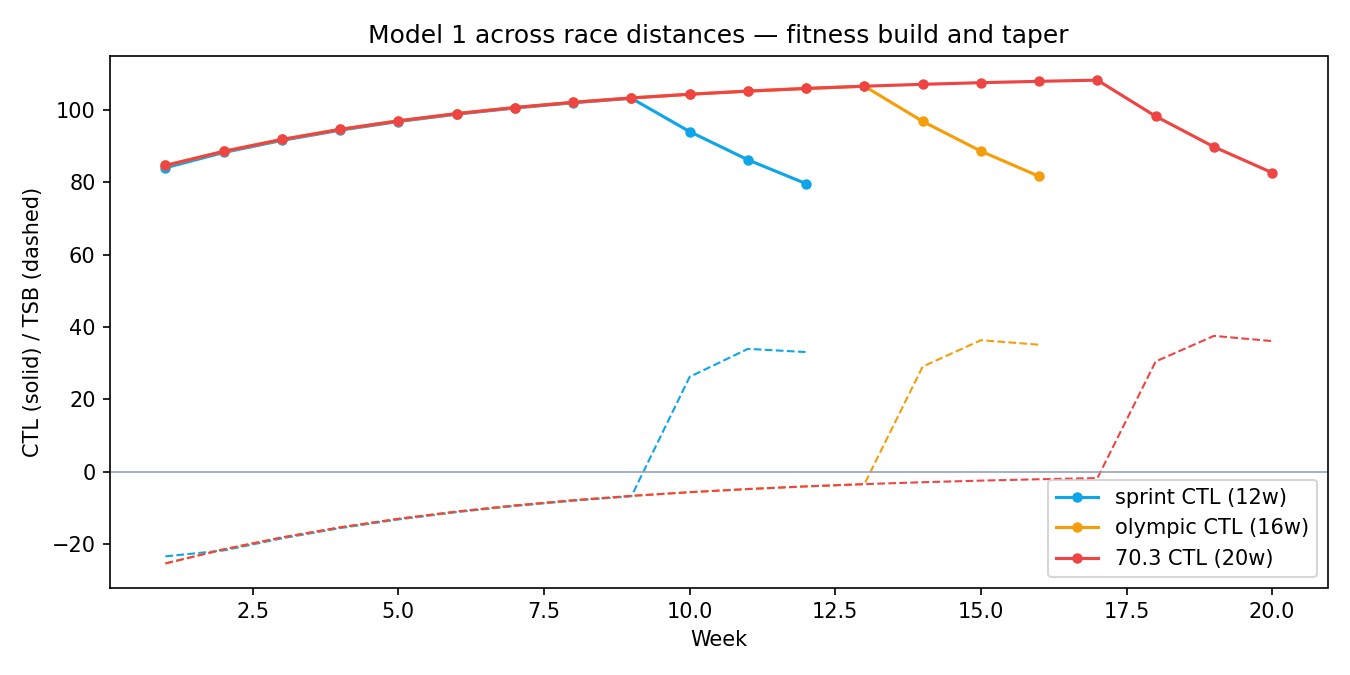
\includegraphics[width=\textwidth]{model1_distance_scenarios.png}
\column{.46\textwidth}
\begin{itemize}\itemsep10pt
  \item \textbf{Sizes:} 12/16/20 weeks, 144--240 vars --- structure invariant
  \item \textbf{$k_2 \in [1,3]$:} race-day TSB stays $35 \pm 2$
  \item \textbf{Cost ranging:} plan invariant for $k_1 \in [0.68, 1.56]$,
        $k_2 \in [1.29, 2.95]$
  \item \textbf{Solve times:} all $< 10$ ms
\end{itemize}
\end{columns}
\end{frame}

\note{\gr Η εκφώνηση ζητάει να «παίξουμε» με το μοντέλο, οπότε: τρία είδη
διαταραχής.

Μέγεθος. Ξανάτρεξα τον μακρόκυκλο σε 12, 16 και 20 εβδομάδες --- από 144 μέχρι
240 μεταβλητές. Οι μεγαλύτεροι ορίζοντες βοηθούν, η αντικειμενική πάει από μείον
13,5 σε μείον 10,4, με φθίνουσες αποδόσεις, και η δομή χτίσιμο-και-μετά-taper
είναι πανομοιότυπη και στις τρεις. Δηλαδή η ποιοτική απάντηση δεν εξαρτάται από
τον ορίζοντα που έτυχε να διαλέξω.

Βαθμονόμηση της αντικειμενικής. Το k2 είναι η παράμετρος για την οποία είμαι πιο
ανασφαλής, οπότε το σάρωσα από 1 έως 3: η φόρμα την ημέρα του αγώνα μετακινείται
ελάχιστα, 35 συν πλην 2. Το βάθος του taper το καθορίζουν οι περιορισμοί --- τα
ελάχιστα της εβδομάδας αγώνα --- όχι η αντικειμενική, κάτι που με καθησυχάζει
επειδή τους περιορισμούς τους έχω μετρήσει.

Και τυπικό cost ranging, κατευθείαν από την ύλη: η βέλτιστη βάση επιβιώνει για k1
οπουδήποτε από 0,68 έως 1,56 και k2 από 1,29 έως 2,95. Τα δύο λιγότερο μετρήσιμα
νούμερα του μοντέλου μπορούν να μεταβληθούν κατά παράγοντα δύο χωρίς να αλλάξει
ούτε μία μεταβλητή.

Όλα λύνονται σε λιγότερο από δέκα χιλιοστά του δευτερολέπτου, οπότε τίποτα από
αυτά δεν μου κόστισε.}

\begin{frame}{Integrating the pipeline: coherence \& fixed point}
\textbf{Do the three objectives agree?}
\begin{itemize}\itemsep5pt
  \item $E = k_E\text{CTL}$ ignores fatigue $\Rightarrow$ four different plans,
        \textbf{same 140.2 min}
  \item $E = E_0 + k_E(\text{CTL}_T - \lambda\,\text{ATL}_T)$ is affine in $p_T$
        \textbf{iff} $\lambda = k_2/k_1$
  \item $E > 0$ needs $\lambda < 1.75$, so $k_2 = 2$ is \emph{incoherent};
        cost ranging licenses $\lambda = 1.5$ --- \textbf{changing no variable}
\end{itemize}
\vspace{6pt}
\textbf{Which model comes first?} Iterate.
\begin{center}\small
\begin{tabular}{clrlr}
\toprule
Iter. & Macrocycle & Weeks & Selected A-race & Outcome\\
\midrule
1 & olympic & 16 & R14 Costa Navarino (70.3) & re-plan as 70.3\\
2 & 70.3 & 20 & R14 Costa Navarino (70.3) & \textbf{fixed point}\\
\bottomrule
\end{tabular}
\end{center}
\end{frame}

\note{\gr Δύο προβλήματα ολοκλήρωσης, που τα θεωρώ το πιο ενδιαφέρον κομμάτι της
εργασίας, επειδή και τα δύο ανακαλύφθηκαν με έλεγχο και όχι με υπόθεση.

Πρώτον, η συνέπεια. Το Μοντέλο 1 μεγιστοποιεί έναν δείκτη απόδοσης· το Μοντέλο 3
ελαχιστοποιεί χρόνο αγώνα. Συμφωνούν; Το δοκίμασα: παρήγαγα τέσσερα αρκετά
διαφορετικά προπονητικά πλάνα και τα έδωσα στο Μοντέλο 3, και τα τέσσερα έδωσαν
τα ίδια 140,2 λεπτά. Το Μοντέλο 3 ήταν τυφλό στην προπόνηση --- επειδή το
ενεργειακό budget ήταν k-E επί CTL, που αγνοεί τελείως την κόπωση. Μπορούσες να
κάνεις taper ή να μην κάνεις και ο αγώνας έβγαινε ίδιος. Αυτό είναι σπασμένη
αλυσίδα.

Η διόρθωση είναι ένα μικρό θεώρημα. Κάνε το budget να εξαρτάται από τη φόρμα:
E-μηδέν συν k-E επί CTL μείον λάμδα επί ATL. Τότε το budget είναι γνησίως αύξουσα
αφινική συνάρτηση της αντικειμενικής του Μοντέλου 1 ακριβώς όταν το λάμδα ισούται
με k2 προς k1 --- και σε αυτή την περίπτωση η μεγιστοποίηση της απόδοσης είναι
αποδεδειγμένα το ίδιο με την ελαχιστοποίηση του χρόνου. Τα μοντέλα
ευθυγραμμίζονται εξ ορισμού, όχι στην τύχη.

Υπάρχει όμως μια παγίδα, και είναι ωραία. Το budget πρέπει να μένει θετικό, που
απαιτεί λάμδα μικρότερο από CTL προς ATL, δηλαδή 1,75. Το k2 που είχα υποθέσει
ίσο με 2 δίνει λάμδα 2 --- ασυνεπές. Άρα το θεώρημα δεν ευθυγραμμίζει απλώς τα
μοντέλα, απορρίπτει μια παράμετρο που είχα διαλέξει. Και εδώ αποδίδει το cost
ranging της προηγούμενης διαφάνειας: λέει ότι το k2 οπουδήποτε από 1,29 έως 2,95
αφήνει το πλάνο αμετάβλητο. Οπότε βάζω λάμδα 1,5, η αλυσίδα γίνεται συνεπής, και
δεν κουνιέται ούτε μία από τις 144 μεταβλητές.

Δεύτερον, η κυκλικότητα. Ο αγώνας-στόχος ορίζει το μήκος του μακρόκυκλου για το
Μοντέλο 1, αλλά το Μοντέλο 1 τροφοδοτεί την πύλη ετοιμότητας του Μοντέλου 2 που
επιλέγει τον αγώνα-στόχο. Αντί να υποθέσω σειρά, έκανα επανάληψη μέχρι σταθερό
σημείο --- δύο επαναλήψεις. Και η επανάληψη βρήκε πραγματικό λάθος: είχα υποθέσει
16 εβδομάδες για ολυμπιακή, αλλά ο αγώνας-στόχος που επιλέγει το ημερολόγιο είναι
70.3, που θέλει 20 εβδομάδες. Αν είχα υποθέσει σειρά, αυτό θα έμενε κρυφό.}

% ---------------------------------------------------------------- payoff
\begin{frame}{What the models actually recommend}
\begin{itemize}\itemsep9pt
  \item \textbf{Train more, much easier.} 6.6 h/wk at 37\% hard
        $\rightarrow$ 9.0 h/wk at \textbf{15\%}
  \item \textbf{More hours are worthless} above 10.5 h/wk --- recovery is what binds
  \item \textbf{Build endurance, not watts.} $+1$ CTL $=$ 69--84 s; $+1$ W $\approx 0$ above 260 W
  \item \textbf{Ride Z3, run hard, fuel 75 g/h.} The 70.3 positive split cost 29 min
  \item \textbf{Protect the calendar, not the budget.} Conflict dual 56.4 vs.\ 0.094/EUR
\end{itemize}
\end{frame}

\note{\gr Αν πάρω στα σοβαρά τη δική μου εργασία, να τι αλλάζει από τη Δευτέρα.

Η πρώτη γραμμή είναι αυτή που πονάει. Αυτή τη στιγμή προπονούμαι 6,6 ώρες την
εβδομάδα με το 37 τοις εκατό σκληρό. Το μοντέλο λέει 9 ώρες με 15 τοις εκατό
σκληρό. Είμαι αντι-πολωμένος --- προπονούμαι πολύ λίγο και πολύ δυνατά. Είναι η
μία αλλαγή με τη μεγαλύτερη απόδοση, και δεν θα την πίστευα χωρίς τις σκιώδεις
τιμές.

Δεύτερον, πρέπει να σταματήσω να ψάχνω κι άλλες ώρες προπόνησης πάνω από τις
δέκα μισή· αξίζουν κυριολεκτικά μηδέν. Ο δεσμευτικός πόρος είναι η ικανότητα
αποκατάστασης.

Τρίτον, από τη σάρωση των βατ: δουλειά αντοχής, όχι threshold ισχύς.

Τέταρτον, εκτέλεση αγώνα: ποδήλατο στη ζώνη 3, κράτα το για το τρέξιμο, σταθερός
ρυθμός, και 75 γραμμάρια υδατανθράκων την ώρα. Το θετικό σπλιτ μου στο 70.3
κόστισε 29 λεπτά.

Πέμπτον, διαπραγματεύσου ημερομηνίες αντί να κυνηγάς χρήματα --- 56,4 έναντι
0,094.

Και μία διόρθωση σχεδιασμού που την αποκάλυψε μόνο η επανάληψη σταθερού σημείου:
παράλειψε το Ντουμπάι στην αρχή της σεζόν γιατί δεν θα προλάβω να είμαι έτοιμος,
και αν ο αγώνας-στόχος είναι 70.3, χτίσε 20 εβδομάδες, όχι 16.}

\begin{frame}{Conclusions}
\begin{itemize}\itemsep10pt
  \item Three coupled models on \textbf{real personal data}
  \item Spanning the syllabus: LP \& Simplex, duality \& sensitivity,
        IP \& Branch \& Bound, network flows \& total unimodularity
  \item The optimizer \textbf{re-derives coaching wisdom} --- periodization,
        polarization, ``steady bike, hard run''
  \item Duals name the real bottlenecks: \emph{recovery}, \emph{calendar space},
        \emph{endurance}
  \item Reproducible: \texttt{python -m src.run\_all}, 60 tests
\end{itemize}
\vspace{6pt}
\begin{center}
{\footnotesize\url{https://github.com/manos1503/triathlon-optimization}}

\vspace{6pt}
\Large Thank you --- questions?
\end{center}
\end{frame}

\note{\gr Κλείνοντας. Τρία συζευγμένα μοντέλα, χτισμένα πάνω σε πραγματικά
προσωπικά δεδομένα και όχι σε σχολικό παράδειγμα, και μαζί καλύπτουν ουσιαστικά
όλη την ύλη: LP και Simplex, δυϊκότητα και ανάλυση ευαισθησίας, ακέραιο
προγραμματισμό με Branch and Bound και τομές, και δίκτυα ροής με ολική
μονοπαραγοντικότητα.

Δύο πράγματα που δεν τα περίμενα όταν ξεκίνησα. Ο optimizer ξαναβγάζει
προπονητική γνώση που δεν του την είπε κανείς --- περιοδικότητα, πολωμένη ένταση,
σταθερό ποδήλατο και δυνατό τρέξιμο. Και οι δυϊκές τιμές διέψευσαν συστηματικά τη
διαίσθησή μου για το τι με περιορίζει: όχι ο χρόνος, όχι τα χρήματα, αλλά η
ικανότητα αποκατάστασης, ο χώρος στο ημερολόγιο, και η αντοχή.

Όλα τρέχουν με μία εντολή και καλύπτονται από 60 tests. Σας ευχαριστώ --- είμαι
στη διάθεσή σας για ερωτήσεις.}

% ---------------------------------------------------------------- backup
\appendix
\begin{frame}{Backup: limitations}
\begin{itemize}\itemsep8pt
  \item \textbf{Weekly} time step for the Banister dynamics
  \item \textbf{Sequential} pipeline, not joint optimization
  \item \textbf{Constructed parameters} in Models 2--3 (race values, zone speeds, $k_E$)
  \item The LP's $+35$ TSB over-taper --- traced to race-week minimums
\end{itemize}
\end{frame}

\note{\gr Ημερήσια ανάλυση θα μετακινούσε τις σταθερές εξομάλυνσης αλλά όχι τη
δομή. Η από κοινού βελτιστοποίηση προπόνησης και ημερολογίου είναι φυσική και
αρκετά μεγαλύτερη επέκταση MIP --- αυτή είναι η προφανής συνέχεια. Οι
κατασκευασμένες παράμετροι είναι τεκμηριωμένες ως παραδοχές, και η ανάλυση
ευαισθησίας υπάρχει ακριβώς για να δείξει ποια συμπεράσματα επιβιώνουν όταν τις
διαταράξω. Και το υπερβολικό taper είναι τεχνούργημα περιορισμού, όχι εννοιολογικό
ελάττωμα του μοντέλου.}

\begin{frame}{Backup: alternative optima \& heuristic benchmark}
\textbf{Alternative optima:} fix $p_T = p^\ast$, re-solve min/max total hours
\begin{center}
same performance with \textbf{124.2 h} or \textbf{162.3 h} of season training
\end{center}
\vspace{8pt}
\textbf{vs.\ a standard coaching heuristic:}
\begin{itemize}\itemsep5pt
  \item violates the fatigue ceiling in \textbf{13 of 16 weeks}
  \item $p_T = -69.5$ vs.\ optimal $-11.4$
  \item but its race-day TSB $+21$ is inside the coaching band; the LP's $+35$ is not
\end{itemize}
\end{frame}

\note{\gr Ο εκφυλισμός γίνεται ορατός: καθηλώνω την αντικειμενική στη βέλτιστη
τιμή της και μετά ελαχιστοποιώ και μεγιστοποιώ τις συνολικές ώρες προπόνησης υπό
αυτόν τον περιορισμό. Και τα δύο είναι βέλτιστα πλάνα, και διαφέρουν κατά 38 ώρες
προπόνησης μέσα στη σεζόν. Αυτό είναι πραγματικό κενό αποδοτικότητας που η
αντικειμενική από μόνη της δεν το βλέπει.

Ο ευρετικός κανόνας είναι αυτό που θα έγραφε ένας λογικός προπονητής --- γέμισε
τις διαθέσιμες ώρες, 20/45/35 στα αθλήματα, 80/15/5 στις εντάσεις. Σπάει το ταβάνι
κόπωσης σε 13 από τις 16 εβδομάδες, που είναι χρόνια υπερπροπόνηση, και βαθμολογεί
πολύ χειρότερα. Δίκαια όμως, φέρνει τη φόρμα της ημέρας του αγώνα μέσα στην
αποδεκτή προπονητική ζώνη ενώ το δικό μου LP όχι --- που είναι ακριβώς το ερώτημα
ευαισθησίας του k2 από πριν.}

\end{document}
"
%       -> presentation-notes.pdf: the same slides with the Greek speaker notes
%          (xelatex, because the notes are in Greek and need a Unicode font)
%
% presentation-notes.pdf is a private rehearsal aid and is NOT committed.
%
% Design rule for this deck: the slide is the evidence, the speaker is the
% argument. Anything that is a sentence rather than a number, a name or a
% figure belongs in \note{}, not on screen.

\documentclass[10pt,aspectratio=169]{beamer}

\usetheme{Madrid}
\usecolortheme{seahorse}
\setbeamertemplate{navigation symbols}{}
\usepackage{amsmath,amssymb}
\usepackage{graphicx}
\usepackage{booktabs}

\ifdefined\shownotes
  \setbeameroption{show notes}
  \usepackage{fontspec}
  % Any installed font with Greek coverage; Helvetica ships with macOS.
  % Override on another machine, e.g. \def\notesfont{DejaVu Sans}
  \providecommand{\notesfont}{Helvetica}
  \newfontfamily\gr{\notesfont}
\else
  \providecommand{\gr}{}
\fi

\graphicspath{{../results/figures/}}

\definecolor{accent}{RGB}{30,60,140}
\setbeamercolor{frametitle}{fg=white,bg=accent}
\setbeamercolor{title}{fg=white,bg=accent}

% one-line takeaway strip under a figure
\newcommand{\takeaway}[1]{\vspace{2pt}\begin{center}\small\textbf{#1}\end{center}}

\title[Triathlon Optimization]{Optimal Resource Allocation and Scheduling\\
       of Athletic Activities, with an Application to Triathlon}
\subtitle{\normalsize Linear and 0--1 Integer Programming models for training
          load, race calendar and race pacing}
\author[E. Vichos]{Emmanouil Vichos (AM 1100830)}
\institute[UPatras]{Linear and Combinatorial Optimization --- University of Patras\\
                    Supervisor: Prof.\ S.\ Daskalaki}
\date{\today}

\begin{document}

\begin{frame}
\titlepage
\end{frame}

\note{\gr Καλημέρα σας. Η εργασία μου εφαρμόζει γραμμικό και ακέραιο
προγραμματισμό στο τρίαθλο --- και μάλιστα όχι σε πλασματικά δεδομένα: σε
δεκαπέντε μήνες δικής μου προπόνησης και σε τρεις αγώνες που πραγματικά έτρεξα.
Τρεις αποφάσεις, τρία μοντέλα, μία αλυσίδα.}

% ---------------------------------------------------------------- overview
\begin{frame}{Three decisions, one athlete}
\begin{enumerate}\itemsep8pt
  \item<1-> \textbf{How to train} --- hours per sport, per intensity, per week
  \item<2-> \textbf{Which races to enter} --- a season under money and recovery limits
  \item<3-> \textbf{How to race} --- spend a finite energy reserve over three legs
\end{enumerate}
\vspace{14pt}
\onslide<4->{
\begin{center}\large
\textbf{Model 1 (LP)} $\;\rightarrow\;$ \textbf{Model 2 (0--1 MIP)} $\;\rightarrow\;$ \textbf{Model 3 (LP)}\\[2pt]
\small training load \hfill race calendar \hfill pacing strategy
\end{center}}
\end{frame}

\note{\gr Οι τρεις αποφάσεις δεν είναι ανεξάρτητες, και αυτό ακριβώς είναι το
νόημα της εργασίας. Η φυσική κατάσταση χτίζεται αργά ενώ η κόπωση γρήγορα, οπότε
η προπόνηση είναι ένα δυναμικό trade-off σε ορίζοντα 12 έως 20 εβδομάδων.

Η κατάσταση φόρμας που βγάζει το Μοντέλο 1 κάνει μετά δύο πράγματα: καθορίζει σε
ποιους αγώνες είμαι έτοιμος να κατέβω, και ορίζει το ενεργειακό budget που έχω
διαθέσιμο την ημέρα του αγώνα. Άρα τα βέλη είναι πραγματικές συζεύξεις, όχι
αφηγηματικό στολίδι.}

% ---------------------------------------------------------------- data
\begin{frame}{Real data: 15 months of my own training}
\begin{columns}
\column{.55\textwidth}
\begin{itemize}\itemsep6pt
  \item Strava export: \textbf{598 activities}, 574 usable
  \item Banister training impulse per activity
  \item Fitness CTL ($\tau{=}42$d), fatigue ATL ($\tau{=}7$d)
  \item Today: CTL $78.1$, ATL $91.5$, \textbf{TSB $-13.4$}
\end{itemize}
\column{.42\textwidth}
\centering\small
\begin{tabular}{lrrr}
\toprule
$r_{db}$/h & easy & mod & hard\\
\midrule
swim & 43.5 & $94.1^\ast$ & $136.6^\ast$\\
bike & 68.3 & 86.9 & $142.7^\ast$\\
run  & 81.6 & 102.8 & $166.0^\ast$\\
\bottomrule
\end{tabular}

\vspace{4pt}
{\scriptsize load rate per hour \quad $^\ast$theoretical (sparse data)}
\end{columns}
\end{frame}

\note{\gr Το export είναι 598 δραστηριότητες από τον Οκτώβριο του 2023 μέχρι τον
Ιούνιο του 2026· οι 574 επιβιώνουν του καθαρισμού. Κάθε μία παίρνει ένα Banister
training impulse --- διάρκεια επί το heart rate reserve επί έναν εκθετικό
συντελεστή. Δύο εκθετικές εξομαλύνσεις αυτής της σειράς δίνουν το CTL με σταθερά
42 ημερών και το ATL με σταθερά 7 ημερών· η διαφορά τους είναι το TSB, η φόρμα.
Αυτή τη στιγμή είμαι σε καλή κατάσταση αλλά κουρασμένος: μείον 13,4.

Ο πίνακας δεξιά είναι η γέφυρα από τα δεδομένα στο μοντέλο: ρυθμός φόρτισης ανά
ώρα, ανά άθλημα, ανά ζώνη έντασης. Οι ζώνες κόβονται ως προς threshold καρδιακό
παλμό ξεχωριστά για κάθε άθλημα --- 173 στο τρέξιμο, 166 στο ποδήλατο, 164 στο
κολύμπι --- γιατί ο ίδιος παλμός δεν σημαίνει το ίδιο πράγμα μέσα στο νερό και
πάνω στο ποδήλατο.

Τα κελιά με αστερίσκο είναι εκεί που έχω λίγα δεδομένα και χρειάστηκε να τα
ορίσω από τη βιβλιογραφία. Τα επισημαίνω επειδή είναι τα πιο αδύναμα inputs του
Μοντέλου 1.}

% ---------------------------------------------------------------- model 1
\begin{frame}{Model 1 --- training-load allocation (LP)}
\textbf{Variables} \quad hours $h_{dbw} \ge 0$: 3 sports $\times$ 3 buckets
$\times$ 16 weeks $= 144$
\vspace{6pt}

\textbf{Banister dynamics, as linear equalities}
\[
L_w = \sum_{d,b} r_{db} h_{dbw}, \qquad
\text{CTL}_w = \lambda_c \text{CTL}_{w-1} + (1{-}\lambda_c)\tfrac{L_w}{7}, \qquad
\text{ATL}_w = \lambda_a \text{ATL}_{w-1} + (1{-}\lambda_a)\tfrac{L_w}{7}
\]

\textbf{Objective} \quad
$\max\; p_T = k_1 \text{CTL}_T - k_2 \text{ATL}_T$
\vspace{6pt}

\textbf{Constraints} \quad weekly hour ceilings $\cdot$ per-sport min/max $\cdot$
80/20 polarization $\cdot$ $\text{ATL} \le 110$ $\cdot$ ramp $\le +10\%$/week
$\cdot$ taper caps
\end{frame}

\note{\gr Εκατόν σαράντα τέσσερις μεταβλητές, όλες συνεχείς και μη αρνητικές.

Το σημαντικό σημείο μοντελοποίησης είναι η δεύτερη γραμμή. Οι αναδρομές του
Banister είναι εκθετικές εξομαλύνσεις, και η εκθετική εξομάλυνση είναι γραμμική
ως προς το φορτίο. Άρα η φυσιολογία μπαίνει στο LP ως ακριβείς ισότητες --- δεν
προσεγγίζω κάποιο μη γραμμικό σύστημα, η δυναμική είναι πράγματι γραμμική ως
προς τις μεταβλητές απόφασής μου.

Για την αντικειμενική συνάρτηση: το προφανές θα ήταν να μεγιστοποιήσω τη φόρμα,
το TSB, δηλαδή CTL μείον ATL. Αυτό όμως είναι εκφυλισμένο --- το βέλτιστο είναι
να μην κάνω τίποτα, γιατί η ξεκούραση μηδενίζει το ATL. Γι' αυτό τα σταθμίζω
χωριστά, k1 επί CTL μείον k2 επί ATL, με το k2 μεγαλύτερο από το k1, που
μεταφράζεται ότι η κόπωση βλάπτει την ημέρα του αγώνα περισσότερο απ' όσο
βοηθάει η φόρμα. Θα επανέλθω στο αν αυτά τα βάρη στέκουν.

Οι περιορισμοί είναι η προπονητική πρακτική διατυπωμένη τυπικά: ταβάνι
εβδομαδιαίων ωρών, κατώφλι και πλαφόν ανά άθλημα ώστε να μη μηδενιστεί το
κολύμπι, ο κανόνας πόλωσης 80/20, ένα σκληρό ταβάνι κόπωσης, ο κανόνας αύξησης
10\% την εβδομάδα, και υποχρεωτικό taper στις δύο τελευταίες εβδομάδες.}

\begin{frame}{Model 1 --- the optimizer discovers periodization}
\centering
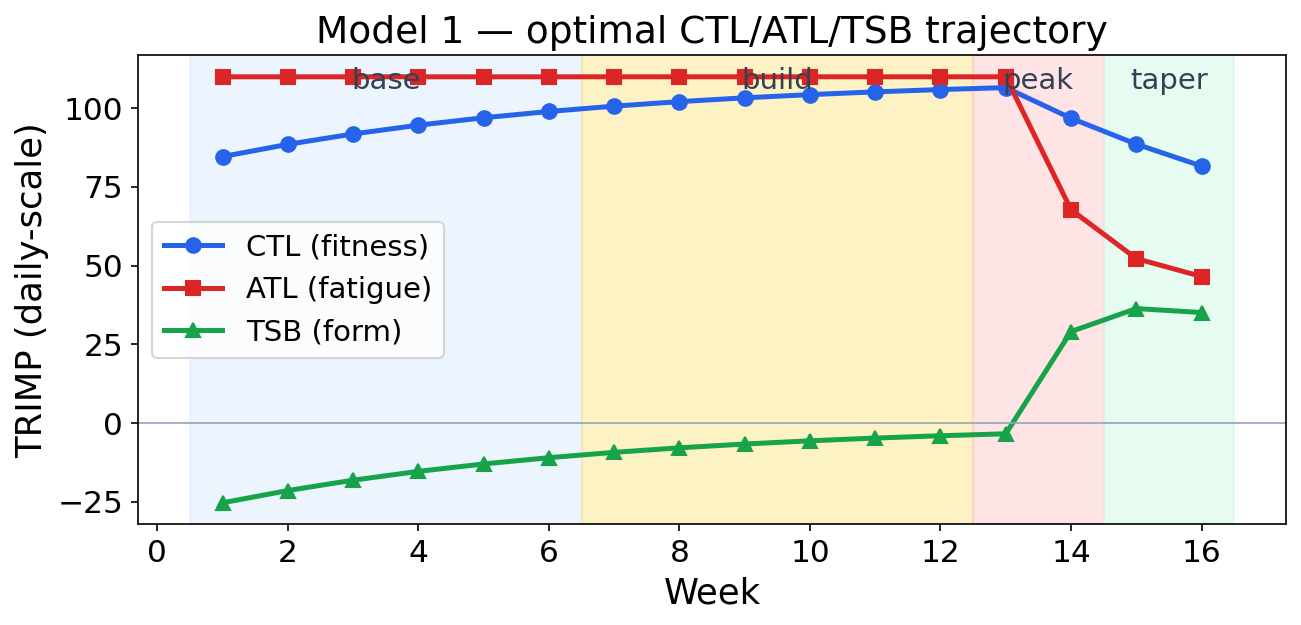
\includegraphics[width=.72\textwidth]{model1_trajectory.png}
\takeaway{Nobody told it to periodize. Week 14 tapers by choice.}
\end{frame}

\note{\gr Αυτό είναι το αγαπημένο μου αποτέλεσμα σε όλη την εργασία. Πουθενά στο
μοντέλο δεν γράφει «κάνε περιοδικότητα». Οι περιορισμοί είναι τοπικοί --- ένας
ρυθμός αύξησης, ένα ταβάνι, ένα κατώφλι --- και ο optimizer παράγει μόνος του
τον κλασικό μακρόκυκλο: κυλάει πάνω στο ταβάνι κόπωσης για δεκατρείς εβδομάδες,
ανεβάζοντας το CTL από 78 στο 107, και μετά κάνει taper.

Και προσέξτε την εβδομάδα 14. Μόνο οι εβδομάδες 15 και 16 είναι αναγκασμένες να
κάνουν taper. Η 14 κάνει taper επειδή το LP υπολογίζει ότι η κόπωση την ημέρα
του αγώνα κοστίζει περισσότερο απ' ό,τι αξίζει η φόρμα που θα αγόραζαν εκείνες
οι ώρες. Δηλαδή το μοντέλο ξαναβγάζει μόνο του προπονητική γνώση, από καθαρή
αριθμητική. Η φόρμα την ημέρα του αγώνα βγαίνει συν 35.}

\begin{frame}{Model 1 --- duality in action}
\begin{columns}
\column{.5\textwidth}
\centering
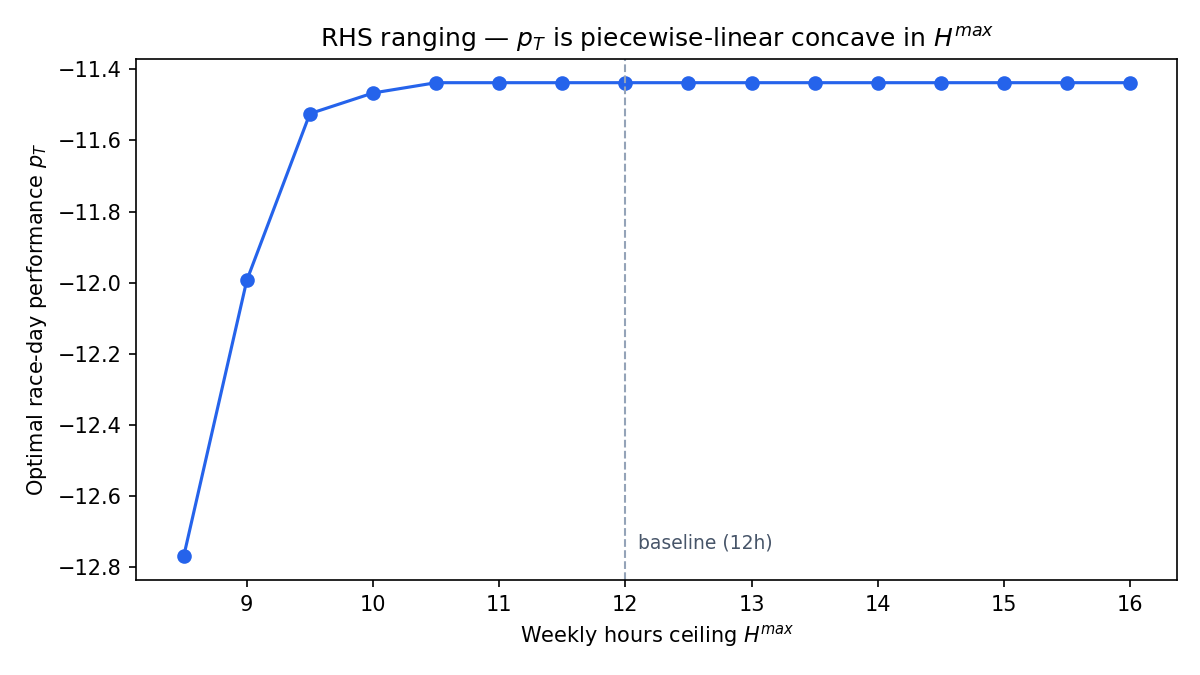
\includegraphics[width=\textwidth]{model1_rhs_ranging.png}
\column{.48\textwidth}
\textbf{RHS ranging:} the hours ceiling, 8--16 h
\begin{itemize}\itemsep6pt
  \item piecewise-linear, concave
  \item slopes $1.55 \to 0.94 \to 0.12 \to 0$
  \item flat above \textbf{10.5 h/week}
\end{itemize}
\vspace{10pt}
\begin{center}
\emph{Recovery capacity, not free time,\\ is what limits this athlete.}
\end{center}
\end{columns}
\end{frame}

\note{\gr Εδώ είναι η ανάλυση ευαισθησίας του μαθήματος, εφαρμοσμένη σε ένα
ερώτημα που με αφορά πραγματικά: αξίζει να ψάξω να βρω κι άλλες ώρες για
προπόνηση;

Μεταβάλλω το δεξί μέλος του περιορισμού των εβδομαδιαίων ωρών από 8 έως 16 και
σχεδιάζω τη βέλτιστη τιμή. Βγαίνει το σχήμα που προβλέπει η θεωρία: κατά
τμήματα γραμμική και κοίλη, επειδή κάθε σημείο καμπής είναι μια αλλαγή βάσης. Οι
κλίσεις είναι οι σκιώδεις τιμές: 1,55 μετά 0,94 μετά 0,12 και μετά μηδέν.

Η απάντηση βρίσκεται στις 10,5 ώρες. Από εκεί και πάνω η σκιώδης τιμή είναι
μηδέν: οι επιπλέον ώρες δεν αξίζουν τίποτα, γιατί το ταβάνι του ATL δεσμεύει
πριν προλάβει να δεσμεύσει το ταβάνι του χρόνου. Το στενό μου σημείο δεν είναι
το πρόγραμμά μου, είναι το πόσο γρήγορα ανακάμπτω.

Να αναφέρω και μία ακόμα δυϊκή τιμή: οι μεγαλύτερες σκιώδεις τιμές όλου του
μοντέλου είναι στους περιορισμούς ελάχιστης προπόνησης της εβδομάδας του αγώνα
--- μείον 12,9 ανά αναγκαστική ώρα τρεξίματος στην εβδομάδα 16. Το μοντέλο θέλει
απόλυτη ξεκούραση κι εγώ το υποχρεώνω να προπονηθεί.}

% ---------------------------------------------------------------- model 2
\begin{frame}{Model 2 --- race-calendar selection (0--1 MIP)}
\textbf{17 candidate races}, binary $x_i$
\[
\max \sum_i \underbrace{q_i(\alpha\,\text{pts}_i + \beta\,\text{strat}_i
+ \gamma\,\text{enj}_i + \varphi\,\text{fit}_i)}_{\text{weather-risk-adjusted value}} x_i
\]
\begin{itemize}\itemsep6pt
  \item \textbf{two knapsacks:} $\le 2500$ EUR, $\le 12$ vacation days
  \item \textbf{recovery spacing:} $x_i + x_j \le 1$; $\le 2$ races/month; $\ge 1$ A-race
  \item \textbf{readiness gate from Model 1:} projected CTL must reach the class
\end{itemize}
\end{frame}

\note{\gr Δεκαεπτά υποψήφιοι αγώνες --- ελληνικοί, ευρωπαϊκοί και δύο
υπερατλαντικοί --- ο καθένας με μία δυαδική μεταβλητή.

Η αξία κάθε αγώνα είναι τέσσερα σταθμισμένα συστατικά: βαθμοί παγκόσμιας
κατάταξης, στρατηγική σημασία, πόσο θα τον ευχαριστηθώ, και πόσο μου ταιριάζει η
διαδρομή. Το τελευταίο δεν είναι αίσθηση: υπολογίζεται από αντικειμενικά
δεδομένα διαδρομής, υψομετρική διαφορά ανά χιλιόμετρο σε σχέση με τη δική μου
προτίμηση σε επίπεδες διαδρομές. Και όλο αυτό πολλαπλασιάζεται με το q, έναν
συντελεστή καιρικού ρίσκου, ώστε ένας αγώνας με ιστορικό ακυρώσεων ή ακραίας
ζέστης να προεξοφλείται.

Τρεις οικογένειες περιορισμών. Δύο σακίδια --- χρήματα και ημέρες άδειας ---
που κάνουν το πρόβλημα δισδιάστατο knapsack. Ανά ζεύγος περιορισμοί αποθεραπείας,
μία, δύο ή τέσσερις εβδομάδες ανάλογα με την κατηγορία απόστασης, γραμμένοι με
τον τυπικό περιορισμό σύγκρουσης: x-i συν x-j το πολύ ένα. Και η πύλη
ετοιμότητας: το προβλεπόμενο CTL από το Μοντέλο 1 πρέπει να φτάνει την απαίτηση
της κατηγορίας --- εδώ ακριβώς μπαίνει φυσικά το Μοντέλο 1 μέσα στο Μοντέλο 2.
Αυτή η πύλη αποκλείει ένα 70.3 υψηλής αξίας στην αρχή της σεζόν: απλούστατα δεν
θα προλάβω να είμαι έτοιμος.}

\begin{frame}{Model 2 --- optimal season}
\centering
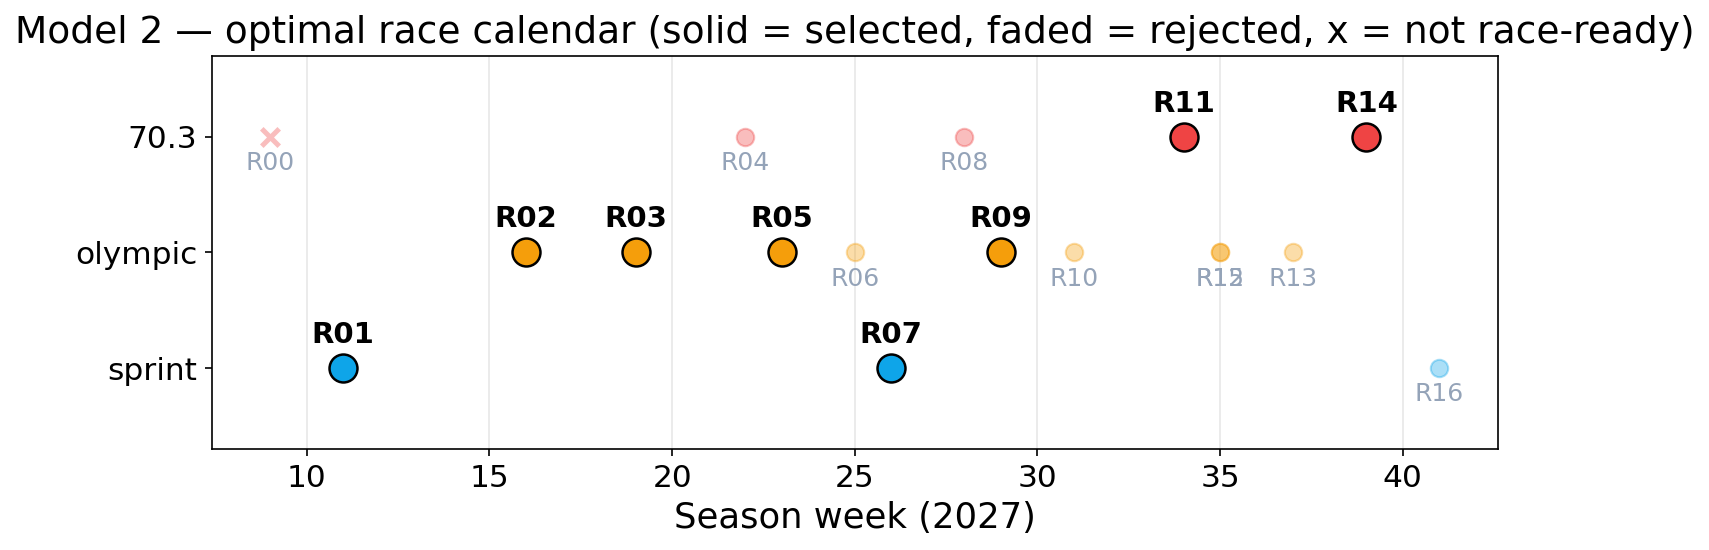
\includegraphics[width=.78\textwidth]{model2_calendar.png}
\takeaway{8 of 17 races $\cdot$ value 571.7 $\cdot$ 2250/2500 EUR $\cdot$ 11/12 days}
\end{frame}

\note{\gr Οκτώ αγώνες από τους δεκαεπτά, συνολική αξία 571,7. Ξοδεύει 2250 από τα
2500 ευρώ και 11 από τις 12 ημέρες άδειας --- άρα και τα δύο σακίδια είναι σχεδόν
γεμάτα, αλλά κανένα δεν δεσμεύει ακριβώς, κάτι που θα έχει σημασία σε δύο
διαφάνειες.

Η ενδιαφέρουσα απόφαση είναι το φθινόπωρο. Το Πανελλήνιο Πρωτάθλημα και το 70.3
της περιοχής μου είναι αρκετά κοντά ώστε ο περιορισμός αποθεραπείας να απαγορεύει
και τα δύο. Ο optimizer κρατάει το 70.3.

Τα «χι» είναι αγώνες για τους οποίους δεν είμαι αρκετά έτοιμος· οι ξεθωριασμένοι
κύκλοι είναι αγώνες που θα μπορούσε να πληρώσει αλλά επέλεξε να μην τους
αγοράσει.}

\begin{frame}{Model 2 --- why Branch \& Bound is needed}
\begin{columns}
\column{.52\textwidth}
\centering
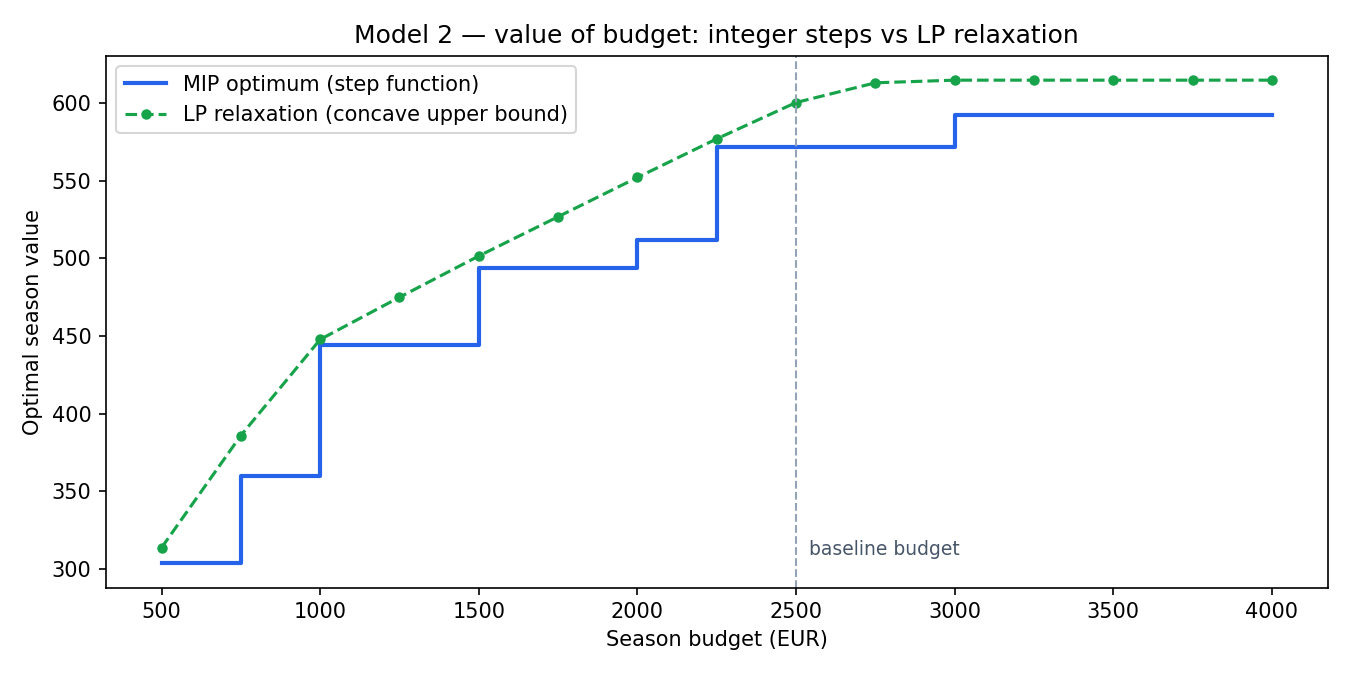
\includegraphics[width=\textwidth]{model2_budget_sweep.png}
\column{.46\textwidth}
\begin{itemize}\itemsep8pt
  \item LP $600.5$ vs.\ MIP $571.7$:\\ \textbf{integrality gap 5.0\%}
  \item 8 fractional variables; the champs/70.3 conflict splits \textbf{0.5/0.5}
  \item \textbf{clique cuts} (Bron--Kerbosch): $600.5 \to 591.0$,\\
        gap \textbf{5.04\% $\to$ 3.38\%}
\end{itemize}
\end{columns}
\end{frame}

\note{\gr Γιατί δεν λύνω απλώς τη γραμμική χαλάρωση και στρογγυλοποιώ; Επειδή η
χαλάρωση δίνει 600,5 έναντι πραγματικού βέλτιστου 571,7 --- κενό ακεραιότητας 5
τοις εκατό --- και οκτώ μεταβλητές βγαίνουν κλασματικές. Η σύγκρουση Πρωτάθλημα
εναντίον 70.3 που μόλις περιέγραψα σπάει ακριβώς μισό-μισό: η χαλάρωση παίρνει
μισό από κάθε αγώνα, που δεν σημαίνει τίποτα. Χρειάζεται Branch and Bound.

Το σχήμα είναι η αξία του χρήματος. Το βέλτιστο του MIP είναι κλιμακωτή
συνάρτηση --- οι αγώνες κοστίζουν όσο κοστίζουν, οπότε τα επιπλέον ευρώ δεν
κάνουν τίποτα μέχρι να φτάσουν να πληρώσουν άλλη μία συμμετοχή --- και βρίσκεται
κάτω από την κοίλη καμπύλη της χαλάρωσης. Πάνω από τα 3000 ευρώ τα σκαλοπάτια
σταματούν, γιατί ο δεσμευτικός πόρος αλλάζει από χρήματα σε ημέρες άδειας.

Για τα cutting planes: φτιάχνω τον γράφο συγκρούσεων των περιορισμών αποθεραπείας
και τρέχω Bron--Kerbosch για να βρω τις μέγιστες κλίκες του. Κάθε κλίκα μεγέθους
τρία ή παραπάνω δίνει μια έγκυρη ανισότητα, άθροισμα των x της κλίκας το πολύ
ένα, που κυριαρχεί των ανά ζεύγος περιορισμών. Τέσσερις τέτοιες τομές σφίγγουν τη
χαλάρωση από 600,5 σε 591, κλείνοντας το ένα τρίτο του κενού, και δεν αποκόπτουν
κανένα ακέραιο σημείο --- το βέλτιστο μένει αμετάβλητο.}

\begin{frame}{Model 2 --- the dual problem}
\[
\kappa_i y_\mathcal{B} + \delta_i y_\mathcal{D} + y_{\text{month}(i)}
+ \sum_{j} y_{ij} - [i \in A] y_A \;\ge\; v_i
\]
\begin{center}\small
\emph{a race enters only if its value covers the shadow cost of what it consumes}
\end{center}
\vspace{4pt}
\begin{center}\small
\begin{tabular}{llr}
\toprule
Dual & Meaning & Price\\
\midrule
$y_{13,14}$ & Champs vs.\ Costa Navarino conflict & \textbf{56.40}\\
$y_{06,07}$ & Hamburg vs.\ Thessaloniki conflict & 31.67\\
$y_\mathcal{B}$ & one extra euro & 0.094\\
$y_\mathcal{D}$ & one extra vacation day & $\approx 0$\\
\bottomrule
\end{tabular}
\end{center}
\takeaway{The scarce resource is calendar space --- not money.}
\end{frame}

\note{\gr Η γραμμική χαλάρωση είναι ήδη σε τυπική μορφή, max c-ανάστροφο-x υπό Ax
μικρότερο ή ίσο του b με x μη αρνητικό, οπότε το δυϊκό είναι το σχολικό: min
b-ανάστροφο-y με A-ανάστροφο-y μεγαλύτερο ή ίσο του c. Γράφοντας μία δυϊκή γραμμή
παίρνω την ανισότητα της διαφάνειας, και έχει καθαρή ανάγνωση: ένας αγώνας μπαίνει
στο ημερολόγιο μόνο αν η αξία του καλύπτει το σκιώδες κόστος όλων όσων καταναλώνει
--- budget, ημέρες άδειας, τη θέση του μήνα του, και κάθε σύγκρουση στην οποία
συμμετέχει.

Τώρα διαβάστε τις τιμές. Ένα ευρώ αξίζει 0,094. Μία ημέρα άδειας ουσιαστικά
μηδέν. Αλλά η σύγκρουση αποθεραπείας ανάμεσα στο Πρωτάθλημα και στην Costa
Navarino τιμολογείται στο 56,4 --- τρεις τάξεις μεγέθους πάνω από το ευρώ.

Άρα η διαίσθηση με την οποία ξεκίνησα ήταν λάθος. Υπέθετα ότι ο περιορισμός ήταν
τα χρήματα. Το δυϊκό λέει ότι ο σπάνιος πόρος είναι ο χώρος στο ημερολόγιο: οι
εβδομάδες αποθεραπείας μεταξύ αγώνων. Πρακτικά, το να διαπραγματευτώ ημερομηνίες
αξίζει πολύ περισσότερο από το να βρω χορηγία.}

\begin{frame}{Model 2 --- network-flow extension}
Drop the knapsacks and the monthly cap $\Rightarrow$ only recovery spacing remains:
\begin{center}
\textbf{feasible calendars $=$ paths in a DAG}
\end{center}
\vspace{6pt}
Three methods, identical answer $z = 639.4$:
\begin{enumerate}\itemsep4pt
  \item dynamic programming --- longest path in topological order
  \item \textbf{flow LP, continuous variables --- integral anyway}
  \item restricted 0--1 MIP
\end{enumerate}
\takeaway{Totally unimodular. The knapsacks are what break the structure.}
\end{frame}

\note{\gr Αυτή η διαφάνεια συνδέει την εργασία με το κομμάτι των δικτύων της ύλης.

Αν αφαιρέσω τα δύο σακίδια και το μηνιαίο πλαφόν, και κρατήσω μόνο την
αποθεραπεία, το πρόβλημα αλλάζει τελείως χαρακτήρα. Βάζω τους αγώνες ως κόμβους
σε σειρά εβδομάδας και τραβάω ακμή από τον i στον j όταν το κενό είναι
τουλάχιστον όσο η αποθεραπεία που απαιτεί ο i. Τότε ένα εφικτό ημερολόγιο είναι
ακριβώς μια διαδρομή σε αυτό το κατευθυνόμενο άκυκλο γράφημα, και το καλύτερο
ημερολόγιο είναι η μακρύτερη διαδρομή.

Το έλυσα με τρεις τρόπους και πήρα 639,4 και τις τρεις φορές. Ο μεσαίος είναι το
θεωρητικό σημείο: το έλυσα ως LP ροής με συνεχείς μεταβλητές, χωρίς κανέναν
περιορισμό ακεραιότητας, και η λύση βγήκε ακέραια από μόνη της. Αυτό είναι ολική
μονοπαραγοντικότητα --- ο πίνακας πρόσπτωσης κόμβων-ακμών είναι TU, άρα κάθε
βασική εφικτή λύση είναι ακέραια και κάθε βάση αντιστοιχεί σε ένα συνδετικό
δέντρο. Αυτή ακριβώς είναι η δομή που εκμεταλλεύεται ο Network Simplex. Δεκαοκτώ
κόμβοι, 136 ακμές.

Και αυτό λέει κάτι για το πλήρες μοντέλο: είναι οι περιορισμοί σακιδίου, το
budget και οι ημέρες άδειας, που καταστρέφουν τη δομή δικτύου και επιβάλλουν
Branch and Bound. Χωρίς αυτούς, δεν χρειάζεται καθόλου διακλάδωση.}

% ---------------------------------------------------------------- model 3
\begin{frame}{Model 3 --- race pacing (LP with linearization)}
\textbf{Variables} \quad minutes $t_{\ell z}$: 3 legs $\times$ 5 zones $= 15$
\vspace{4pt}

\textbf{Linearization} \quad within a zone, speed and energy rate are \emph{constants}
\[
\min \sum_{\ell,z} t_{\ell z} + T_1 + T_2
\quad \text{s.t.} \quad
\underbrace{\textstyle\sum_z s_{\ell z} t_{\ell z} \ge d_\ell}_{\text{distances}},\;
\underbrace{\textstyle\sum e_{\ell z} t_{\ell z} \le k_E \cdot \text{CTL}_T}_{\text{energy budget (Model 1)}},\;
\underbrace{\text{Z4+ caps}}_{\text{per leg}},\;
\underbrace{\varphi \cdot G}_{\text{bike} \to \text{run}}
\]
\vspace{-6pt}
\begin{center}\small
bike speed $\propto \phi(\gamma)\cdot(\text{power})^{1/3}$ \quad --- \quad
$\phi(\gamma)$ from the power balance, \textbf{derived, not fitted}
\end{center}
\end{frame}

\note{\gr Εδώ η φυσική είναι μη γραμμική: η σχέση ταχύτητας και ενεργειακού
κόστους είναι καμπύλη, όχι ευθεία. Το κόλπο είναι να διακριτοποιήσω την ένταση
στις πέντε προπονητικές ζώνες. Μέσα σε μια ζώνη, η ταχύτητα και ο ρυθμός
κατανάλωσης είναι σταθερές, άρα και η απόσταση και η ενέργεια γίνονται γραμμικές
ως προς τον χρόνο που ξοδεύω εκεί, και το πρόβλημα ξαναγίνεται LP. Δεκαπέντε
μεταβλητές. Αυτή είναι η κλασική κατά τμήματα γραμμική προσέγγιση του μαθήματος,
και οι ζώνες δεν είναι αυθαίρετες --- είναι οι ζώνες στις οποίες προπονούνται
πραγματικά οι αθλητές.

Δύο όροι αξίζουν κουβέντα. Η ταχύτητα στο ποδήλατο πάει με την κυβική ρίζα της
ισχύος, επειδή η αεροδυναμική αντίσταση πάει με την ταχύτητα στον κύβο --- αν
διπλασιάσεις την ισχύ σου δεν πλησιάζεις καν τον διπλασιασμό της ταχύτητας.

Και το φι του γάμμα είναι ο συντελεστής κλίσης της διαδρομής. Μοντελοποιώ μια
διαδρομή που ανεβαίνει γάμμα μέτρα ανά χιλιόμετρο ως μισή ανηφόρα και μισή
κατηφόρα με σταθερή ισχύ, και παίρνω τον αρμονικό μέσο των δύο ταχυτήτων. Η
αεροδυναμική σταθερά προκύπτει αντίστροφα από τη δική μου ταχύτητα σε επίπεδη
διαδρομή, οπότε τίποτα μέσα στο φι δεν είναι προσαρμοσμένο σε αποτέλεσμα αγώνα.
Αυτό θα έχει σημασία στην επικύρωση, τρεις διαφάνειες πιο κάτω.

Ο τελευταίος όρος είναι η σύζευξη που κάνει το πρόβλημα τρίαθλο και όχι τρεις
ξεχωριστούς αγώνες: κάθε κιλοτζάουλ σκληρής δουλειάς στο ποδήλατο μειώνει το πόσο
μακριά μπορώ μετά να τρέξω.}

\begin{frame}{Model 3 --- ``steady bike, hard run,'' derived}
\centering
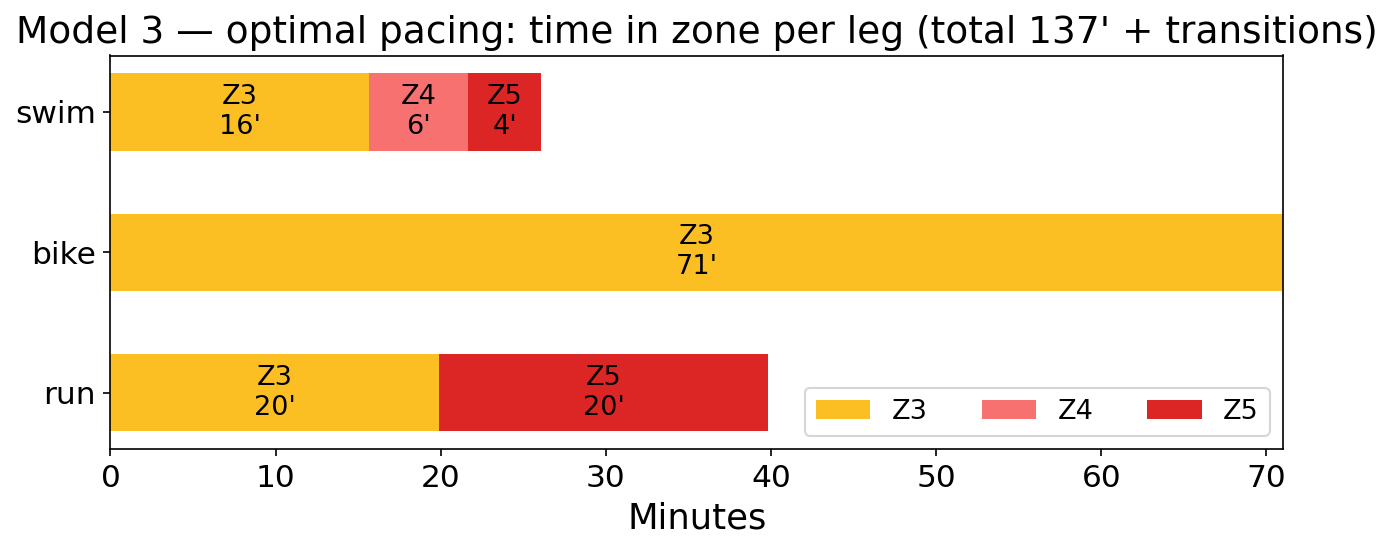
\includegraphics[width=.70\textwidth]{model3_pacing.png}
\takeaway{Bike entirely Z3. Energy budget exhausted \emph{exactly}: 9389 kJ.}
\end{frame}

\note{\gr Ολυμπιακή απόσταση σε 140,4 λεπτά, και το ενεργειακό budget εξαντλείται
ακριβώς --- 9389 κιλοτζάουλ διαθέσιμα, 9389 καταναλωμένα. Ο ενεργειακός
περιορισμός είναι δεσμευτικός, γι' αυτό και η δυϊκή του τιμή είναι το ενδιαφέρον
νούμερο της επόμενης διαφάνειας.

Η δομή της απάντησης είναι το προπονητικό κλισέ «σταθερό ποδήλατο, δυνατό
τρέξιμο», και το LP το βγάζει χωρίς να του το πει κανείς. Το ποδήλατο είναι
εξ ολοκλήρου στη ζώνη 3, τίποτα πιο σκληρό. Γιατί; Για δύο λόγους, και οι δύο
μέσα στο μοντέλο: η κυβική ρίζα σημαίνει ότι το σκληρό ποδήλατο αγοράζει ελάχιστη
ταχύτητα, και ο όρος σύζευξης σημαίνει ότι σου κοστίζει άμεσα απόσταση στο
τρέξιμο. Οπότε ο optimizer ξοδεύει την ένταση εκεί που η ένταση είναι φθηνή,
δηλαδή στο τρέξιμο.}

\begin{frame}{Model 3 --- what is a watt worth?}
\centering
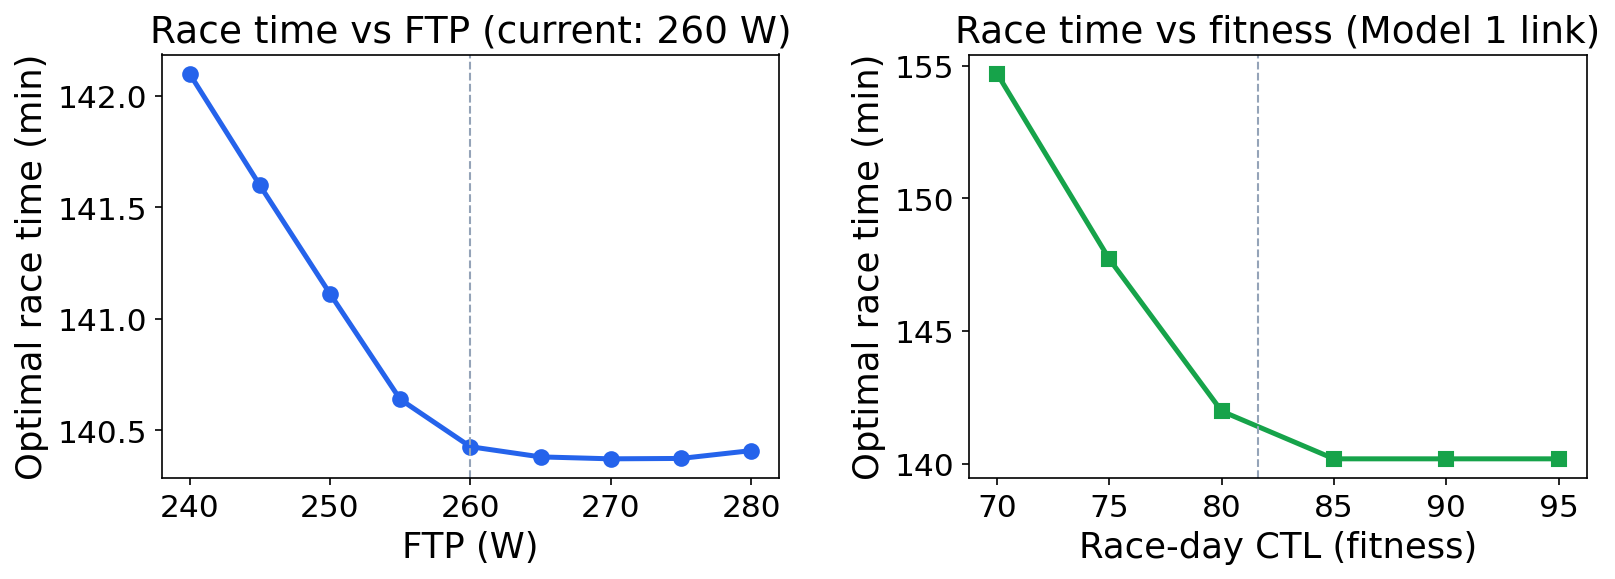
\includegraphics[width=.86\textwidth]{model3_sweeps.png}
\takeaway{$+1$ CTL $=$ 69--84 s. $+1$ W $\approx$ 6 s --- but only below 260 W.}
\end{frame}

\note{\gr Δύο σαρώσεις ευαισθησίας, και οι δύο απαντούν σε ερωτήματα που κάνει
ένας πραγματικός αθλητής.

Αριστερά: τι αξίζει ένα βατ; Κάτω από τα 260 βατ, κάθε επιπλέον βατ threshold
ισχύος αξίζει περίπου έξι δευτερόλεπτα. Πάνω από εκεί, η αξία καταρρέει στο μηδέν.
Αυτό δεν είναι σφάλμα --- είναι ο ενεργειακός περιορισμός. Με σταθερό απόθεμα
κιλοτζάουλ, δεν έχει νόημα να μπορείς να παράγεις περισσότερη ισχύ, γιατί δεν
μπορείς να την τροφοδοτήσεις. Το σκέλος του ποδηλάτου γίνεται ενεργειακά
περιορισμένο αντί για περιορισμένο από ισχύ.

Δεξιά: τι αξίζει μία μονάδα φόρμας; Εξήντα εννιά έως ογδόντα τέσσερα δευτερόλεπτα
ανά μονάδα CTL, και κρατάει μέχρι περίπου CTL 85.

Άρα τα δύο νούμερα μαζί δίνουν ξεκάθαρο προπονητικό συμπέρασμα: χτίσε αντοχή, όχι
μέγιστη ισχύ. Και αυτό βγήκε από σκιώδη τιμή, όχι από γνώμη. Η ίδια η δυϊκή τιμή
της ενέργειας, παρεμπιπτόντως, είναι 0,43 δευτερόλεπτα ανά κιλοτζάουλ.}

\begin{frame}{Model 3 --- validated against three real races}
\begin{center}\small
\begin{tabular}{llrrrrrr}
\toprule
& & \multicolumn{2}{c}{Swim} & \multicolumn{2}{c}{Bike} & \multicolumn{2}{c}{Run}\\
Race & CTL & mdl & act & mdl & act & mdl & act\\
\midrule
Spetsathlon '26 (sprint$^\ast$) & 64.9 & 12.9 & 13.2 & 47.3 & 50.9 & 18.7 & 17.7\\
Epidavros '25 (Olympic) & 55.6 & 27.2 & 25.8 & 88.8 & 91.5 & 38.9 & 42.0\\
70.3 Costa Navarino '25 & 71.4 & 33.3 & 32.9 & 184.6 & 180.3 & 86.4 & \textbf{115.2}\\
\bottomrule
\end{tabular}

{\scriptsize minutes $\cdot$ $^\ast$non-standard 25 km bike}
\end{center}
\vspace{4pt}
\begin{itemize}\itemsep5pt
  \item swim within 0.5 min every time
  \item binding constraint \textbf{switches with distance}: speed caps $\to$ energy
        $\to$ infeasible unfed
  \item the 70.3 run: my \textbf{29-minute} wall is the energy constraint, violated in real life
\end{itemize}
\end{frame}

\note{\gr Αυτό είναι το κομμάτι που δεν θα μπορούσα να κάνω με πλασματικά
δεδομένα. Βρήκα τις τρεις ημέρες αγώνα μέσα στο ακατέργαστο export --- είναι οι
μόνες τρεις μέρες που περιέχουν κολύμπι, ποδήλατο και τρέξιμο --- και πήρα την
κατάσταση φόρμας από την αλυσίδα επεξεργασίας, από την προηγούμενη μέρα. Τίποτα
εδώ δεν ρυθμίστηκε για να δείχνουν ωραία τα νούμερα.

Το κολύμπι πέφτει μέσα σε μισό λεπτό και τις τρεις φορές, που μου λέει ότι τα
μετρημένα κατώφλια είναι σωστά.

Η επιστημονικά ενδιαφέρουσα γραμμή είναι η μεσαία: το ποιος περιορισμός δεσμεύει
αλλάζει με την απόσταση του αγώνα. Στο sprint είναι τα πλαφόν ταχύτητας των
ζωνών --- με περιορίζει η τελική ταχύτητα, όχι το καύσιμο. Στην ολυμπιακή είναι η
ενέργεια. Στο 70.3 το μοντέλο βγαίνει εντελώς ανέφικτο με μόνο την αποθηκευμένη
ενέργεια· λύνεται μόνο αν το ταΐσεις. Και η πρόσληψη που χρειάζεται είναι περίπου
21 κιλοτζάουλ το λεπτό, που μεταφράζεται σε 75 γραμμάρια υδατανθράκων την ώρα ---
την τυπική οδηγία της αθλητικής διατροφής, ανακτημένη από ένα γραμμικό πρόγραμμα
που δεν την είχε ακούσει ποτέ.

Και τώρα η τίμια αποτυχία. Το μοντέλο προβλέπει 86 λεπτά για το τρέξιμο του 70.3·
εγώ έκανα 115. Αλλά δείτε τι συνέβη: μετά το δέκατο χιλιόμετρο πήγα από 4:53 ανά
χιλιόμετρο σε 5:52, με τον παλμό να πέφτει από 162 σε 145. Το να επιβραδύνεις ενώ
ο παλμός σου πέφτει δεν είναι κακή διαχείριση ρυθμού, είναι να σου τελειώνει το
καύσιμο. Άρα αυτά τα 29 λεπτά δεν είναι λάθος του μοντέλου --- είναι εγώ που
παραβίασα τον ενεργειακό περιορισμό στην πραγματικότητα. Το μοντέλο μου λέει πόσο
μου κόστισε.}

\begin{frame}{What the bike residual is made of}
\begin{center}\small
\begin{tabular}{lrrrrr}
\toprule
Bike leg & m/km & no gradient & $\phi(\gamma)$ & 2-param fit & actual\\
\midrule
Spetsathlon (24.4 km) & 15.2 & 43.3 & \textbf{47.3} & 55.0 & 50.9\\
Epidavros (38.7 km) & 15.5 & 78.9 & \textbf{88.8} & 87.7 & 91.5\\
Costa Navarino (88.5 km) & 9.1 & 177.5 & \textbf{184.6} & 180.0 & 180.3\\
\midrule
\multicolumn{2}{l}{total error} & 23.0 min & \textbf{10.6 min} & 8.2 min & \\
\multicolumn{2}{l}{parameters fitted here} & 0 & \textbf{0} & 2 & \\
\bottomrule
\end{tabular}
\end{center}
\vspace{6pt}
\begin{itemize}\itemsep5pt
  \item no gradient $\Rightarrow$ too fast on \textbf{every} course: a missing term, not noise
  \item $\phi(\gamma)$ from physics halves the error with \textbf{zero} fitted parameters
\end{itemize}
\end{frame}

\note{\gr Το ποδήλατο είναι το λιγότερο ακριβές σκέλος, οπότε θέλω να δείξω ότι
ξέρω γιατί, αντί να ελπίζω ότι δεν θα ρωτήσει κανείς.

Το ερώτημα: το υπόλοιπο του ποδηλάτου είναι απλώς θόρυβος, ή λείπει όρος από το
μοντέλο; Δύο στοιχεία λένε ότι λείπει όρος. Πρώτον το μέγεθος --- 23 λεπτά σε
τρεις αγώνες. Δεύτερον, και πιο αποκαλυπτικό, το πρόσημο: αν προσποιηθώ ότι κάθε
διαδρομή είναι επίπεδη, βγαίνω γρηγορότερος και στις τρεις. Ο θόρυβος δεν έχει
πρόσημο.

Ο όρος που λείπει είναι η κλίση, και επίτηδες δεν την κόλλησα εκ των υστέρων.
Ανήκει στη διατύπωση, οπότε το φι του γάμμα είναι μέρος του μοντέλου, παραγόμενο
από το ισοζύγιο ισχύος του ποδηλάτου, με μηδέν παραμέτρους προσαρμοσμένες σε
αυτούς τους αγώνες. Αυτό είναι γνήσιο out-of-sample τεστ και υποδιπλασιάζει το
σφάλμα στα 10,6 λεπτά, με τα υπόλοιπα να πέφτουν πλέον και από τις δύο πλευρές
του μηδενός.

Η τελευταία στήλη είναι ο έλεγχός μου. Προσάρμοσα και μια εμπειρική διόρθωση δύο
παραμέτρων κατευθείαν πάνω σε αυτούς τους τρεις αγώνες --- που είναι ζαβολιά, και
αποτελεί άνω φράγμα του πόσο καλή θα μπορούσε να φανεί οποιαδήποτε τέτοια
διόρθωση. Κερδίζει μόλις 2,4 λεπτά παραπάνω. Άρα η κλίση εξηγεί ουσιαστικά όλο το
ανακτήσιμο σφάλμα, και η παραγόμενη εκδοχή το παίρνει σχεδόν όλο δωρεάν.

Και η μικρή μεροληψία που απομένει εξηγείται κι αυτή: το φι υποθέτει ότι κρατάω
threshold ισχύ στις κατηφόρες, που δεν το κάνει κανείς, οπότε μένω ελαφρώς
αισιόδοξος στις δύο ανηφορικές διαδρομές.}

% ---------------------------------------------------------------- playing with the model
\begin{frame}{Sensitivity across sizes and parameters}
\begin{columns}
\column{.52\textwidth}
\centering
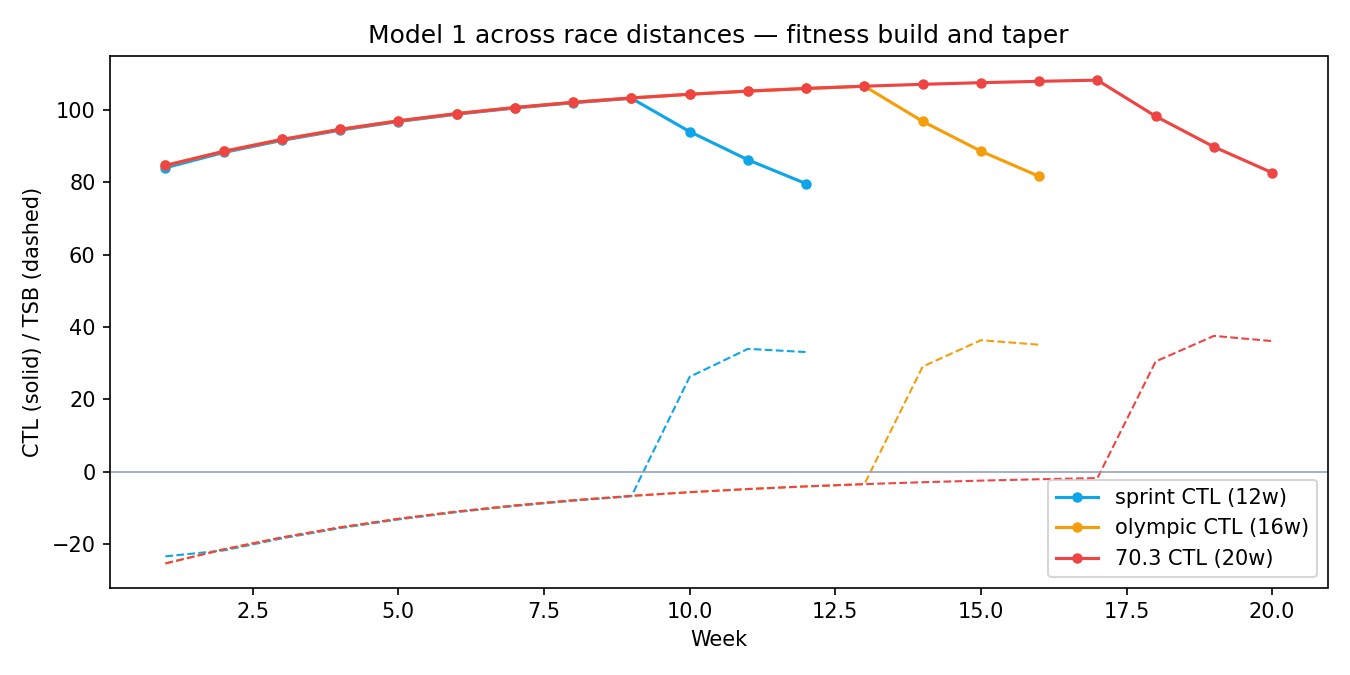
\includegraphics[width=\textwidth]{model1_distance_scenarios.png}
\column{.46\textwidth}
\begin{itemize}\itemsep10pt
  \item \textbf{Sizes:} 12/16/20 weeks, 144--240 vars --- structure invariant
  \item \textbf{$k_2 \in [1,3]$:} race-day TSB stays $35 \pm 2$
  \item \textbf{Cost ranging:} plan invariant for $k_1 \in [0.68, 1.56]$,
        $k_2 \in [1.29, 2.95]$
  \item \textbf{Solve times:} all $< 10$ ms
\end{itemize}
\end{columns}
\end{frame}

\note{\gr Η εκφώνηση ζητάει να «παίξουμε» με το μοντέλο, οπότε: τρία είδη
διαταραχής.

Μέγεθος. Ξανάτρεξα τον μακρόκυκλο σε 12, 16 και 20 εβδομάδες --- από 144 μέχρι
240 μεταβλητές. Οι μεγαλύτεροι ορίζοντες βοηθούν, η αντικειμενική πάει από μείον
13,5 σε μείον 10,4, με φθίνουσες αποδόσεις, και η δομή χτίσιμο-και-μετά-taper
είναι πανομοιότυπη και στις τρεις. Δηλαδή η ποιοτική απάντηση δεν εξαρτάται από
τον ορίζοντα που έτυχε να διαλέξω.

Βαθμονόμηση της αντικειμενικής. Το k2 είναι η παράμετρος για την οποία είμαι πιο
ανασφαλής, οπότε το σάρωσα από 1 έως 3: η φόρμα την ημέρα του αγώνα μετακινείται
ελάχιστα, 35 συν πλην 2. Το βάθος του taper το καθορίζουν οι περιορισμοί --- τα
ελάχιστα της εβδομάδας αγώνα --- όχι η αντικειμενική, κάτι που με καθησυχάζει
επειδή τους περιορισμούς τους έχω μετρήσει.

Και τυπικό cost ranging, κατευθείαν από την ύλη: η βέλτιστη βάση επιβιώνει για k1
οπουδήποτε από 0,68 έως 1,56 και k2 από 1,29 έως 2,95. Τα δύο λιγότερο μετρήσιμα
νούμερα του μοντέλου μπορούν να μεταβληθούν κατά παράγοντα δύο χωρίς να αλλάξει
ούτε μία μεταβλητή.

Όλα λύνονται σε λιγότερο από δέκα χιλιοστά του δευτερολέπτου, οπότε τίποτα από
αυτά δεν μου κόστισε.}

\begin{frame}{Integrating the pipeline: coherence \& fixed point}
\textbf{Do the three objectives agree?}
\begin{itemize}\itemsep5pt
  \item $E = k_E\text{CTL}$ ignores fatigue $\Rightarrow$ four different plans,
        \textbf{same 140.2 min}
  \item $E = E_0 + k_E(\text{CTL}_T - \lambda\,\text{ATL}_T)$ is affine in $p_T$
        \textbf{iff} $\lambda = k_2/k_1$
  \item $E > 0$ needs $\lambda < 1.75$, so $k_2 = 2$ is \emph{incoherent};
        cost ranging licenses $\lambda = 1.5$ --- \textbf{changing no variable}
\end{itemize}
\vspace{6pt}
\textbf{Which model comes first?} Iterate.
\begin{center}\small
\begin{tabular}{clrlr}
\toprule
Iter. & Macrocycle & Weeks & Selected A-race & Outcome\\
\midrule
1 & olympic & 16 & R14 Costa Navarino (70.3) & re-plan as 70.3\\
2 & 70.3 & 20 & R14 Costa Navarino (70.3) & \textbf{fixed point}\\
\bottomrule
\end{tabular}
\end{center}
\end{frame}

\note{\gr Δύο προβλήματα ολοκλήρωσης, που τα θεωρώ το πιο ενδιαφέρον κομμάτι της
εργασίας, επειδή και τα δύο ανακαλύφθηκαν με έλεγχο και όχι με υπόθεση.

Πρώτον, η συνέπεια. Το Μοντέλο 1 μεγιστοποιεί έναν δείκτη απόδοσης· το Μοντέλο 3
ελαχιστοποιεί χρόνο αγώνα. Συμφωνούν; Το δοκίμασα: παρήγαγα τέσσερα αρκετά
διαφορετικά προπονητικά πλάνα και τα έδωσα στο Μοντέλο 3, και τα τέσσερα έδωσαν
τα ίδια 140,2 λεπτά. Το Μοντέλο 3 ήταν τυφλό στην προπόνηση --- επειδή το
ενεργειακό budget ήταν k-E επί CTL, που αγνοεί τελείως την κόπωση. Μπορούσες να
κάνεις taper ή να μην κάνεις και ο αγώνας έβγαινε ίδιος. Αυτό είναι σπασμένη
αλυσίδα.

Η διόρθωση είναι ένα μικρό θεώρημα. Κάνε το budget να εξαρτάται από τη φόρμα:
E-μηδέν συν k-E επί CTL μείον λάμδα επί ATL. Τότε το budget είναι γνησίως αύξουσα
αφινική συνάρτηση της αντικειμενικής του Μοντέλου 1 ακριβώς όταν το λάμδα ισούται
με k2 προς k1 --- και σε αυτή την περίπτωση η μεγιστοποίηση της απόδοσης είναι
αποδεδειγμένα το ίδιο με την ελαχιστοποίηση του χρόνου. Τα μοντέλα
ευθυγραμμίζονται εξ ορισμού, όχι στην τύχη.

Υπάρχει όμως μια παγίδα, και είναι ωραία. Το budget πρέπει να μένει θετικό, που
απαιτεί λάμδα μικρότερο από CTL προς ATL, δηλαδή 1,75. Το k2 που είχα υποθέσει
ίσο με 2 δίνει λάμδα 2 --- ασυνεπές. Άρα το θεώρημα δεν ευθυγραμμίζει απλώς τα
μοντέλα, απορρίπτει μια παράμετρο που είχα διαλέξει. Και εδώ αποδίδει το cost
ranging της προηγούμενης διαφάνειας: λέει ότι το k2 οπουδήποτε από 1,29 έως 2,95
αφήνει το πλάνο αμετάβλητο. Οπότε βάζω λάμδα 1,5, η αλυσίδα γίνεται συνεπής, και
δεν κουνιέται ούτε μία από τις 144 μεταβλητές.

Δεύτερον, η κυκλικότητα. Ο αγώνας-στόχος ορίζει το μήκος του μακρόκυκλου για το
Μοντέλο 1, αλλά το Μοντέλο 1 τροφοδοτεί την πύλη ετοιμότητας του Μοντέλου 2 που
επιλέγει τον αγώνα-στόχο. Αντί να υποθέσω σειρά, έκανα επανάληψη μέχρι σταθερό
σημείο --- δύο επαναλήψεις. Και η επανάληψη βρήκε πραγματικό λάθος: είχα υποθέσει
16 εβδομάδες για ολυμπιακή, αλλά ο αγώνας-στόχος που επιλέγει το ημερολόγιο είναι
70.3, που θέλει 20 εβδομάδες. Αν είχα υποθέσει σειρά, αυτό θα έμενε κρυφό.}

% ---------------------------------------------------------------- payoff
\begin{frame}{What the models actually recommend}
\begin{itemize}\itemsep9pt
  \item \textbf{Train more, much easier.} 6.6 h/wk at 37\% hard
        $\rightarrow$ 9.0 h/wk at \textbf{15\%}
  \item \textbf{More hours are worthless} above 10.5 h/wk --- recovery is what binds
  \item \textbf{Build endurance, not watts.} $+1$ CTL $=$ 69--84 s; $+1$ W $\approx 0$ above 260 W
  \item \textbf{Ride Z3, run hard, fuel 75 g/h.} The 70.3 positive split cost 29 min
  \item \textbf{Protect the calendar, not the budget.} Conflict dual 56.4 vs.\ 0.094/EUR
\end{itemize}
\end{frame}

\note{\gr Αν πάρω στα σοβαρά τη δική μου εργασία, να τι αλλάζει από τη Δευτέρα.

Η πρώτη γραμμή είναι αυτή που πονάει. Αυτή τη στιγμή προπονούμαι 6,6 ώρες την
εβδομάδα με το 37 τοις εκατό σκληρό. Το μοντέλο λέει 9 ώρες με 15 τοις εκατό
σκληρό. Είμαι αντι-πολωμένος --- προπονούμαι πολύ λίγο και πολύ δυνατά. Είναι η
μία αλλαγή με τη μεγαλύτερη απόδοση, και δεν θα την πίστευα χωρίς τις σκιώδεις
τιμές.

Δεύτερον, πρέπει να σταματήσω να ψάχνω κι άλλες ώρες προπόνησης πάνω από τις
δέκα μισή· αξίζουν κυριολεκτικά μηδέν. Ο δεσμευτικός πόρος είναι η ικανότητα
αποκατάστασης.

Τρίτον, από τη σάρωση των βατ: δουλειά αντοχής, όχι threshold ισχύς.

Τέταρτον, εκτέλεση αγώνα: ποδήλατο στη ζώνη 3, κράτα το για το τρέξιμο, σταθερός
ρυθμός, και 75 γραμμάρια υδατανθράκων την ώρα. Το θετικό σπλιτ μου στο 70.3
κόστισε 29 λεπτά.

Πέμπτον, διαπραγματεύσου ημερομηνίες αντί να κυνηγάς χρήματα --- 56,4 έναντι
0,094.

Και μία διόρθωση σχεδιασμού που την αποκάλυψε μόνο η επανάληψη σταθερού σημείου:
παράλειψε το Ντουμπάι στην αρχή της σεζόν γιατί δεν θα προλάβω να είμαι έτοιμος,
και αν ο αγώνας-στόχος είναι 70.3, χτίσε 20 εβδομάδες, όχι 16.}

\begin{frame}{Conclusions}
\begin{itemize}\itemsep10pt
  \item Three coupled models on \textbf{real personal data}
  \item Spanning the syllabus: LP \& Simplex, duality \& sensitivity,
        IP \& Branch \& Bound, network flows \& total unimodularity
  \item The optimizer \textbf{re-derives coaching wisdom} --- periodization,
        polarization, ``steady bike, hard run''
  \item Duals name the real bottlenecks: \emph{recovery}, \emph{calendar space},
        \emph{endurance}
  \item Reproducible: \texttt{python -m src.run\_all}, 60 tests
\end{itemize}
\vspace{6pt}
\begin{center}
{\footnotesize\url{https://github.com/manos1503/triathlon-optimization}}

\vspace{6pt}
\Large Thank you --- questions?
\end{center}
\end{frame}

\note{\gr Κλείνοντας. Τρία συζευγμένα μοντέλα, χτισμένα πάνω σε πραγματικά
προσωπικά δεδομένα και όχι σε σχολικό παράδειγμα, και μαζί καλύπτουν ουσιαστικά
όλη την ύλη: LP και Simplex, δυϊκότητα και ανάλυση ευαισθησίας, ακέραιο
προγραμματισμό με Branch and Bound και τομές, και δίκτυα ροής με ολική
μονοπαραγοντικότητα.

Δύο πράγματα που δεν τα περίμενα όταν ξεκίνησα. Ο optimizer ξαναβγάζει
προπονητική γνώση που δεν του την είπε κανείς --- περιοδικότητα, πολωμένη ένταση,
σταθερό ποδήλατο και δυνατό τρέξιμο. Και οι δυϊκές τιμές διέψευσαν συστηματικά τη
διαίσθησή μου για το τι με περιορίζει: όχι ο χρόνος, όχι τα χρήματα, αλλά η
ικανότητα αποκατάστασης, ο χώρος στο ημερολόγιο, και η αντοχή.

Όλα τρέχουν με μία εντολή και καλύπτονται από 60 tests. Σας ευχαριστώ --- είμαι
στη διάθεσή σας για ερωτήσεις.}

% ---------------------------------------------------------------- backup
\appendix
\begin{frame}{Backup: limitations}
\begin{itemize}\itemsep8pt
  \item \textbf{Weekly} time step for the Banister dynamics
  \item \textbf{Sequential} pipeline, not joint optimization
  \item \textbf{Constructed parameters} in Models 2--3 (race values, zone speeds, $k_E$)
  \item The LP's $+35$ TSB over-taper --- traced to race-week minimums
\end{itemize}
\end{frame}

\note{\gr Ημερήσια ανάλυση θα μετακινούσε τις σταθερές εξομάλυνσης αλλά όχι τη
δομή. Η από κοινού βελτιστοποίηση προπόνησης και ημερολογίου είναι φυσική και
αρκετά μεγαλύτερη επέκταση MIP --- αυτή είναι η προφανής συνέχεια. Οι
κατασκευασμένες παράμετροι είναι τεκμηριωμένες ως παραδοχές, και η ανάλυση
ευαισθησίας υπάρχει ακριβώς για να δείξει ποια συμπεράσματα επιβιώνουν όταν τις
διαταράξω. Και το υπερβολικό taper είναι τεχνούργημα περιορισμού, όχι εννοιολογικό
ελάττωμα του μοντέλου.}

\begin{frame}{Backup: alternative optima \& heuristic benchmark}
\textbf{Alternative optima:} fix $p_T = p^\ast$, re-solve min/max total hours
\begin{center}
same performance with \textbf{124.2 h} or \textbf{162.3 h} of season training
\end{center}
\vspace{8pt}
\textbf{vs.\ a standard coaching heuristic:}
\begin{itemize}\itemsep5pt
  \item violates the fatigue ceiling in \textbf{13 of 16 weeks}
  \item $p_T = -69.5$ vs.\ optimal $-11.4$
  \item but its race-day TSB $+21$ is inside the coaching band; the LP's $+35$ is not
\end{itemize}
\end{frame}

\note{\gr Ο εκφυλισμός γίνεται ορατός: καθηλώνω την αντικειμενική στη βέλτιστη
τιμή της και μετά ελαχιστοποιώ και μεγιστοποιώ τις συνολικές ώρες προπόνησης υπό
αυτόν τον περιορισμό. Και τα δύο είναι βέλτιστα πλάνα, και διαφέρουν κατά 38 ώρες
προπόνησης μέσα στη σεζόν. Αυτό είναι πραγματικό κενό αποδοτικότητας που η
αντικειμενική από μόνη της δεν το βλέπει.

Ο ευρετικός κανόνας είναι αυτό που θα έγραφε ένας λογικός προπονητής --- γέμισε
τις διαθέσιμες ώρες, 20/45/35 στα αθλήματα, 80/15/5 στις εντάσεις. Σπάει το ταβάνι
κόπωσης σε 13 από τις 16 εβδομάδες, που είναι χρόνια υπερπροπόνηση, και βαθμολογεί
πολύ χειρότερα. Δίκαια όμως, φέρνει τη φόρμα της ημέρας του αγώνα μέσα στην
αποδεκτή προπονητική ζώνη ενώ το δικό μου LP όχι --- που είναι ακριβώς το ερώτημα
ευαισθησίας του k2 από πριν.}

\end{document}
"
%       -> presentation-notes.pdf: the same slides with the Greek speaker notes
%          (xelatex, because the notes are in Greek and need a Unicode font)
%
% presentation-notes.pdf is a private rehearsal aid and is NOT committed.
%
% Design rule for this deck: the slide is the evidence, the speaker is the
% argument. Anything that is a sentence rather than a number, a name or a
% figure belongs in \note{}, not on screen.

\documentclass[10pt,aspectratio=169]{beamer}

\usetheme{Madrid}
\usecolortheme{seahorse}
\setbeamertemplate{navigation symbols}{}
\usepackage{amsmath,amssymb}
\usepackage{graphicx}
\usepackage{booktabs}

\ifdefined\shownotes
  \setbeameroption{show notes}
  \usepackage{fontspec}
  % Any installed font with Greek coverage; Helvetica ships with macOS.
  % Override on another machine, e.g. \def\notesfont{DejaVu Sans}
  \providecommand{\notesfont}{Helvetica}
  \newfontfamily\gr{\notesfont}
\else
  \providecommand{\gr}{}
\fi

\graphicspath{{../results/figures/}}

\definecolor{accent}{RGB}{30,60,140}
\setbeamercolor{frametitle}{fg=white,bg=accent}
\setbeamercolor{title}{fg=white,bg=accent}

% one-line takeaway strip under a figure
\newcommand{\takeaway}[1]{\vspace{2pt}\begin{center}\small\textbf{#1}\end{center}}

\title[Triathlon Optimization]{Optimal Resource Allocation and Scheduling\\
       of Athletic Activities, with an Application to Triathlon}
\subtitle{\normalsize Linear and 0--1 Integer Programming models for training
          load, race calendar and race pacing}
\author[E. Vichos]{Emmanouil Vichos (AM 1100830)}
\institute[UPatras]{Linear and Combinatorial Optimization --- University of Patras\\
                    Supervisor: Prof.\ S.\ Daskalaki}
\date{\today}

\begin{document}

\begin{frame}
\titlepage
\end{frame}

\note{\gr Καλημέρα σας. Η εργασία μου εφαρμόζει γραμμικό και ακέραιο
προγραμματισμό στο τρίαθλο --- και μάλιστα όχι σε πλασματικά δεδομένα: σε
δεκαπέντε μήνες δικής μου προπόνησης και σε τρεις αγώνες που πραγματικά έτρεξα.
Τρεις αποφάσεις, τρία μοντέλα, μία αλυσίδα.}

% ---------------------------------------------------------------- overview
\begin{frame}{Three decisions, one athlete}
\begin{enumerate}\itemsep8pt
  \item<1-> \textbf{How to train} --- hours per sport, per intensity, per week
  \item<2-> \textbf{Which races to enter} --- a season under money and recovery limits
  \item<3-> \textbf{How to race} --- spend a finite energy reserve over three legs
\end{enumerate}
\vspace{14pt}
\onslide<4->{
\begin{center}\large
\textbf{Model 1 (LP)} $\;\rightarrow\;$ \textbf{Model 2 (0--1 MIP)} $\;\rightarrow\;$ \textbf{Model 3 (LP)}\\[2pt]
\small training load \hfill race calendar \hfill pacing strategy
\end{center}}
\end{frame}

\note{\gr Οι τρεις αποφάσεις δεν είναι ανεξάρτητες, και αυτό ακριβώς είναι το
νόημα της εργασίας. Η φυσική κατάσταση χτίζεται αργά ενώ η κόπωση γρήγορα, οπότε
η προπόνηση είναι ένα δυναμικό trade-off σε ορίζοντα 12 έως 20 εβδομάδων.

Η κατάσταση φόρμας που βγάζει το Μοντέλο 1 κάνει μετά δύο πράγματα: καθορίζει σε
ποιους αγώνες είμαι έτοιμος να κατέβω, και ορίζει το ενεργειακό budget που έχω
διαθέσιμο την ημέρα του αγώνα. Άρα τα βέλη είναι πραγματικές συζεύξεις, όχι
αφηγηματικό στολίδι.}

% ---------------------------------------------------------------- data
\begin{frame}{Real data: 15 months of my own training}
\begin{columns}
\column{.55\textwidth}
\begin{itemize}\itemsep6pt
  \item Strava export: \textbf{598 activities}, 574 usable
  \item Banister training impulse per activity
  \item Fitness CTL ($\tau{=}42$d), fatigue ATL ($\tau{=}7$d)
  \item Today: CTL $78.1$, ATL $91.5$, \textbf{TSB $-13.4$}
\end{itemize}
\column{.42\textwidth}
\centering\small
\begin{tabular}{lrrr}
\toprule
$r_{db}$/h & easy & mod & hard\\
\midrule
swim & 43.5 & $94.1^\ast$ & $136.6^\ast$\\
bike & 68.3 & 86.9 & $142.7^\ast$\\
run  & 81.6 & 102.8 & $166.0^\ast$\\
\bottomrule
\end{tabular}

\vspace{4pt}
{\scriptsize load rate per hour \quad $^\ast$theoretical (sparse data)}
\end{columns}
\end{frame}

\note{\gr Το export είναι 598 δραστηριότητες από τον Οκτώβριο του 2023 μέχρι τον
Ιούνιο του 2026· οι 574 επιβιώνουν του καθαρισμού. Κάθε μία παίρνει ένα Banister
training impulse --- διάρκεια επί το heart rate reserve επί έναν εκθετικό
συντελεστή. Δύο εκθετικές εξομαλύνσεις αυτής της σειράς δίνουν το CTL με σταθερά
42 ημερών και το ATL με σταθερά 7 ημερών· η διαφορά τους είναι το TSB, η φόρμα.
Αυτή τη στιγμή είμαι σε καλή κατάσταση αλλά κουρασμένος: μείον 13,4.

Ο πίνακας δεξιά είναι η γέφυρα από τα δεδομένα στο μοντέλο: ρυθμός φόρτισης ανά
ώρα, ανά άθλημα, ανά ζώνη έντασης. Οι ζώνες κόβονται ως προς threshold καρδιακό
παλμό ξεχωριστά για κάθε άθλημα --- 173 στο τρέξιμο, 166 στο ποδήλατο, 164 στο
κολύμπι --- γιατί ο ίδιος παλμός δεν σημαίνει το ίδιο πράγμα μέσα στο νερό και
πάνω στο ποδήλατο.

Τα κελιά με αστερίσκο είναι εκεί που έχω λίγα δεδομένα και χρειάστηκε να τα
ορίσω από τη βιβλιογραφία. Τα επισημαίνω επειδή είναι τα πιο αδύναμα inputs του
Μοντέλου 1.}

% ---------------------------------------------------------------- model 1
\begin{frame}{Model 1 --- training-load allocation (LP)}
\textbf{Variables} \quad hours $h_{dbw} \ge 0$: 3 sports $\times$ 3 buckets
$\times$ 16 weeks $= 144$
\vspace{6pt}

\textbf{Banister dynamics, as linear equalities}
\[
L_w = \sum_{d,b} r_{db} h_{dbw}, \qquad
\text{CTL}_w = \lambda_c \text{CTL}_{w-1} + (1{-}\lambda_c)\tfrac{L_w}{7}, \qquad
\text{ATL}_w = \lambda_a \text{ATL}_{w-1} + (1{-}\lambda_a)\tfrac{L_w}{7}
\]

\textbf{Objective} \quad
$\max\; p_T = k_1 \text{CTL}_T - k_2 \text{ATL}_T$
\vspace{6pt}

\textbf{Constraints} \quad weekly hour ceilings $\cdot$ per-sport min/max $\cdot$
80/20 polarization $\cdot$ $\text{ATL} \le 110$ $\cdot$ ramp $\le +10\%$/week
$\cdot$ taper caps
\end{frame}

\note{\gr Εκατόν σαράντα τέσσερις μεταβλητές, όλες συνεχείς και μη αρνητικές.

Το σημαντικό σημείο μοντελοποίησης είναι η δεύτερη γραμμή. Οι αναδρομές του
Banister είναι εκθετικές εξομαλύνσεις, και η εκθετική εξομάλυνση είναι γραμμική
ως προς το φορτίο. Άρα η φυσιολογία μπαίνει στο LP ως ακριβείς ισότητες --- δεν
προσεγγίζω κάποιο μη γραμμικό σύστημα, η δυναμική είναι πράγματι γραμμική ως
προς τις μεταβλητές απόφασής μου.

Για την αντικειμενική συνάρτηση: το προφανές θα ήταν να μεγιστοποιήσω τη φόρμα,
το TSB, δηλαδή CTL μείον ATL. Αυτό όμως είναι εκφυλισμένο --- το βέλτιστο είναι
να μην κάνω τίποτα, γιατί η ξεκούραση μηδενίζει το ATL. Γι' αυτό τα σταθμίζω
χωριστά, k1 επί CTL μείον k2 επί ATL, με το k2 μεγαλύτερο από το k1, που
μεταφράζεται ότι η κόπωση βλάπτει την ημέρα του αγώνα περισσότερο απ' όσο
βοηθάει η φόρμα. Θα επανέλθω στο αν αυτά τα βάρη στέκουν.

Οι περιορισμοί είναι η προπονητική πρακτική διατυπωμένη τυπικά: ταβάνι
εβδομαδιαίων ωρών, κατώφλι και πλαφόν ανά άθλημα ώστε να μη μηδενιστεί το
κολύμπι, ο κανόνας πόλωσης 80/20, ένα σκληρό ταβάνι κόπωσης, ο κανόνας αύξησης
10\% την εβδομάδα, και υποχρεωτικό taper στις δύο τελευταίες εβδομάδες.}

\begin{frame}{Model 1 --- the optimizer discovers periodization}
\centering
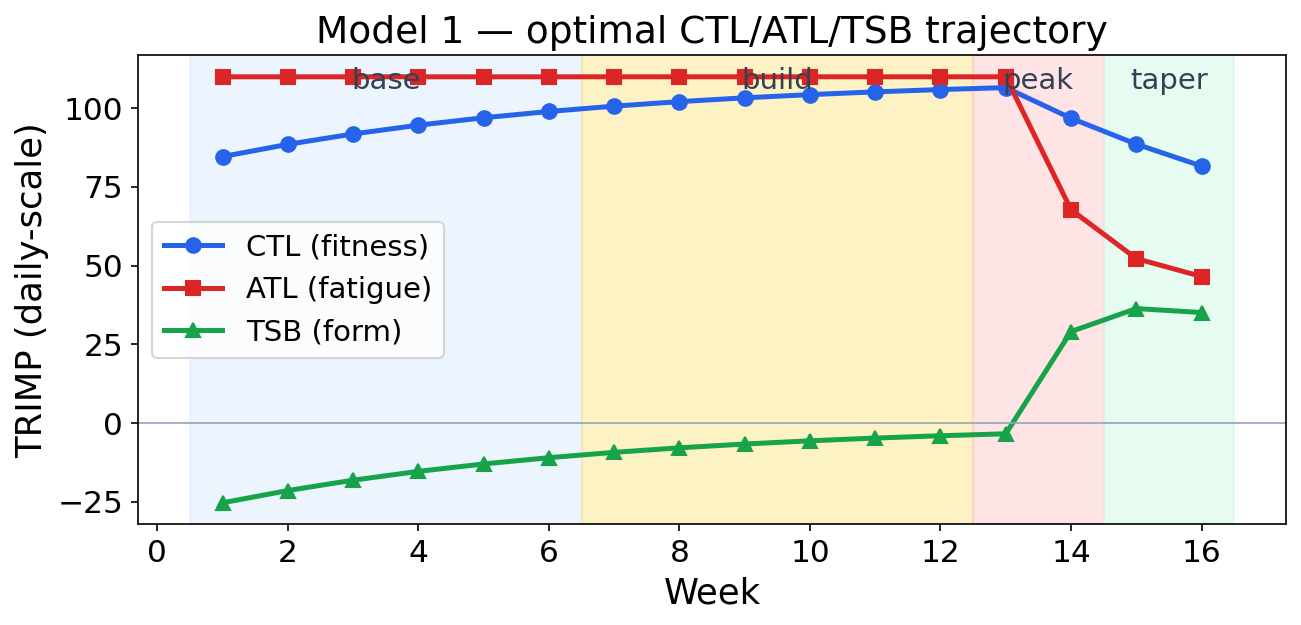
\includegraphics[width=.72\textwidth]{model1_trajectory.png}
\takeaway{Nobody told it to periodize. Week 14 tapers by choice.}
\end{frame}

\note{\gr Αυτό είναι το αγαπημένο μου αποτέλεσμα σε όλη την εργασία. Πουθενά στο
μοντέλο δεν γράφει «κάνε περιοδικότητα». Οι περιορισμοί είναι τοπικοί --- ένας
ρυθμός αύξησης, ένα ταβάνι, ένα κατώφλι --- και ο optimizer παράγει μόνος του
τον κλασικό μακρόκυκλο: κυλάει πάνω στο ταβάνι κόπωσης για δεκατρείς εβδομάδες,
ανεβάζοντας το CTL από 78 στο 107, και μετά κάνει taper.

Και προσέξτε την εβδομάδα 14. Μόνο οι εβδομάδες 15 και 16 είναι αναγκασμένες να
κάνουν taper. Η 14 κάνει taper επειδή το LP υπολογίζει ότι η κόπωση την ημέρα
του αγώνα κοστίζει περισσότερο απ' ό,τι αξίζει η φόρμα που θα αγόραζαν εκείνες
οι ώρες. Δηλαδή το μοντέλο ξαναβγάζει μόνο του προπονητική γνώση, από καθαρή
αριθμητική. Η φόρμα την ημέρα του αγώνα βγαίνει συν 35.}

\begin{frame}{Model 1 --- duality in action}
\begin{columns}
\column{.5\textwidth}
\centering
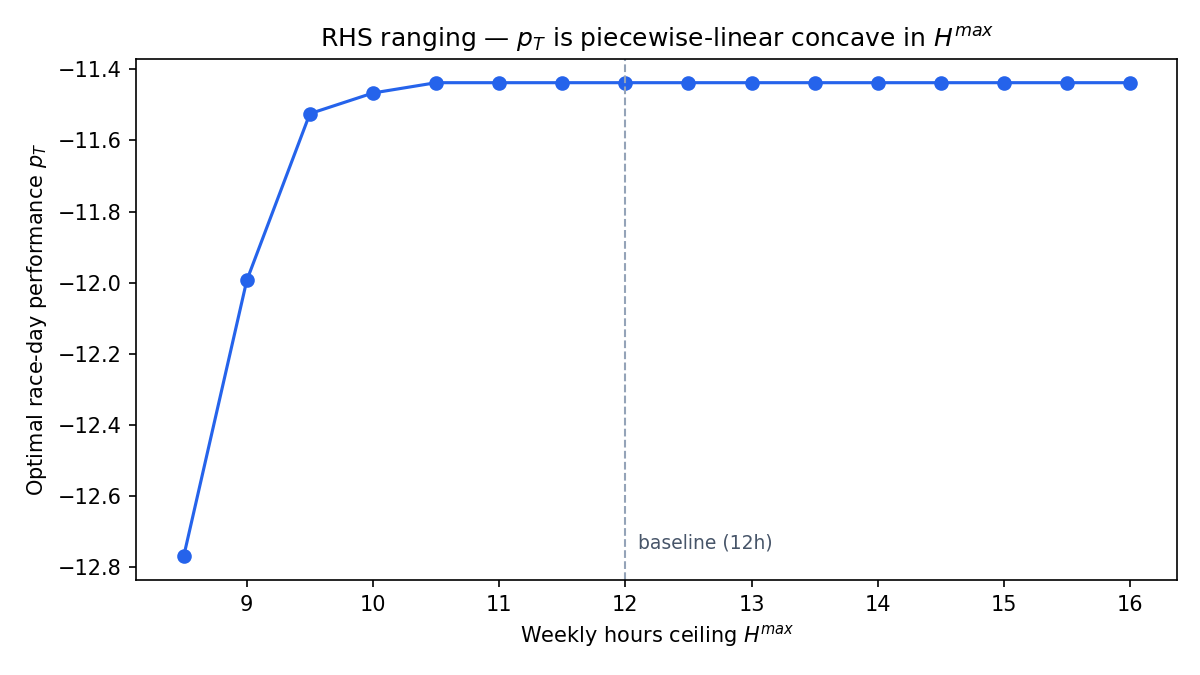
\includegraphics[width=\textwidth]{model1_rhs_ranging.png}
\column{.48\textwidth}
\textbf{RHS ranging:} the hours ceiling, 8--16 h
\begin{itemize}\itemsep6pt
  \item piecewise-linear, concave
  \item slopes $1.55 \to 0.94 \to 0.12 \to 0$
  \item flat above \textbf{10.5 h/week}
\end{itemize}
\vspace{10pt}
\begin{center}
\emph{Recovery capacity, not free time,\\ is what limits this athlete.}
\end{center}
\end{columns}
\end{frame}

\note{\gr Εδώ είναι η ανάλυση ευαισθησίας του μαθήματος, εφαρμοσμένη σε ένα
ερώτημα που με αφορά πραγματικά: αξίζει να ψάξω να βρω κι άλλες ώρες για
προπόνηση;

Μεταβάλλω το δεξί μέλος του περιορισμού των εβδομαδιαίων ωρών από 8 έως 16 και
σχεδιάζω τη βέλτιστη τιμή. Βγαίνει το σχήμα που προβλέπει η θεωρία: κατά
τμήματα γραμμική και κοίλη, επειδή κάθε σημείο καμπής είναι μια αλλαγή βάσης. Οι
κλίσεις είναι οι σκιώδεις τιμές: 1,55 μετά 0,94 μετά 0,12 και μετά μηδέν.

Η απάντηση βρίσκεται στις 10,5 ώρες. Από εκεί και πάνω η σκιώδης τιμή είναι
μηδέν: οι επιπλέον ώρες δεν αξίζουν τίποτα, γιατί το ταβάνι του ATL δεσμεύει
πριν προλάβει να δεσμεύσει το ταβάνι του χρόνου. Το στενό μου σημείο δεν είναι
το πρόγραμμά μου, είναι το πόσο γρήγορα ανακάμπτω.

Να αναφέρω και μία ακόμα δυϊκή τιμή: οι μεγαλύτερες σκιώδεις τιμές όλου του
μοντέλου είναι στους περιορισμούς ελάχιστης προπόνησης της εβδομάδας του αγώνα
--- μείον 12,9 ανά αναγκαστική ώρα τρεξίματος στην εβδομάδα 16. Το μοντέλο θέλει
απόλυτη ξεκούραση κι εγώ το υποχρεώνω να προπονηθεί.}

% ---------------------------------------------------------------- model 2
\begin{frame}{Model 2 --- race-calendar selection (0--1 MIP)}
\textbf{17 candidate races}, binary $x_i$
\[
\max \sum_i \underbrace{q_i(\alpha\,\text{pts}_i + \beta\,\text{strat}_i
+ \gamma\,\text{enj}_i + \varphi\,\text{fit}_i)}_{\text{weather-risk-adjusted value}} x_i
\]
\begin{itemize}\itemsep6pt
  \item \textbf{two knapsacks:} $\le 2500$ EUR, $\le 12$ vacation days
  \item \textbf{recovery spacing:} $x_i + x_j \le 1$; $\le 2$ races/month; $\ge 1$ A-race
  \item \textbf{readiness gate from Model 1:} projected CTL must reach the class
\end{itemize}
\end{frame}

\note{\gr Δεκαεπτά υποψήφιοι αγώνες --- ελληνικοί, ευρωπαϊκοί και δύο
υπερατλαντικοί --- ο καθένας με μία δυαδική μεταβλητή.

Η αξία κάθε αγώνα είναι τέσσερα σταθμισμένα συστατικά: βαθμοί παγκόσμιας
κατάταξης, στρατηγική σημασία, πόσο θα τον ευχαριστηθώ, και πόσο μου ταιριάζει η
διαδρομή. Το τελευταίο δεν είναι αίσθηση: υπολογίζεται από αντικειμενικά
δεδομένα διαδρομής, υψομετρική διαφορά ανά χιλιόμετρο σε σχέση με τη δική μου
προτίμηση σε επίπεδες διαδρομές. Και όλο αυτό πολλαπλασιάζεται με το q, έναν
συντελεστή καιρικού ρίσκου, ώστε ένας αγώνας με ιστορικό ακυρώσεων ή ακραίας
ζέστης να προεξοφλείται.

Τρεις οικογένειες περιορισμών. Δύο σακίδια --- χρήματα και ημέρες άδειας ---
που κάνουν το πρόβλημα δισδιάστατο knapsack. Ανά ζεύγος περιορισμοί αποθεραπείας,
μία, δύο ή τέσσερις εβδομάδες ανάλογα με την κατηγορία απόστασης, γραμμένοι με
τον τυπικό περιορισμό σύγκρουσης: x-i συν x-j το πολύ ένα. Και η πύλη
ετοιμότητας: το προβλεπόμενο CTL από το Μοντέλο 1 πρέπει να φτάνει την απαίτηση
της κατηγορίας --- εδώ ακριβώς μπαίνει φυσικά το Μοντέλο 1 μέσα στο Μοντέλο 2.
Αυτή η πύλη αποκλείει ένα 70.3 υψηλής αξίας στην αρχή της σεζόν: απλούστατα δεν
θα προλάβω να είμαι έτοιμος.}

\begin{frame}{Model 2 --- optimal season}
\centering
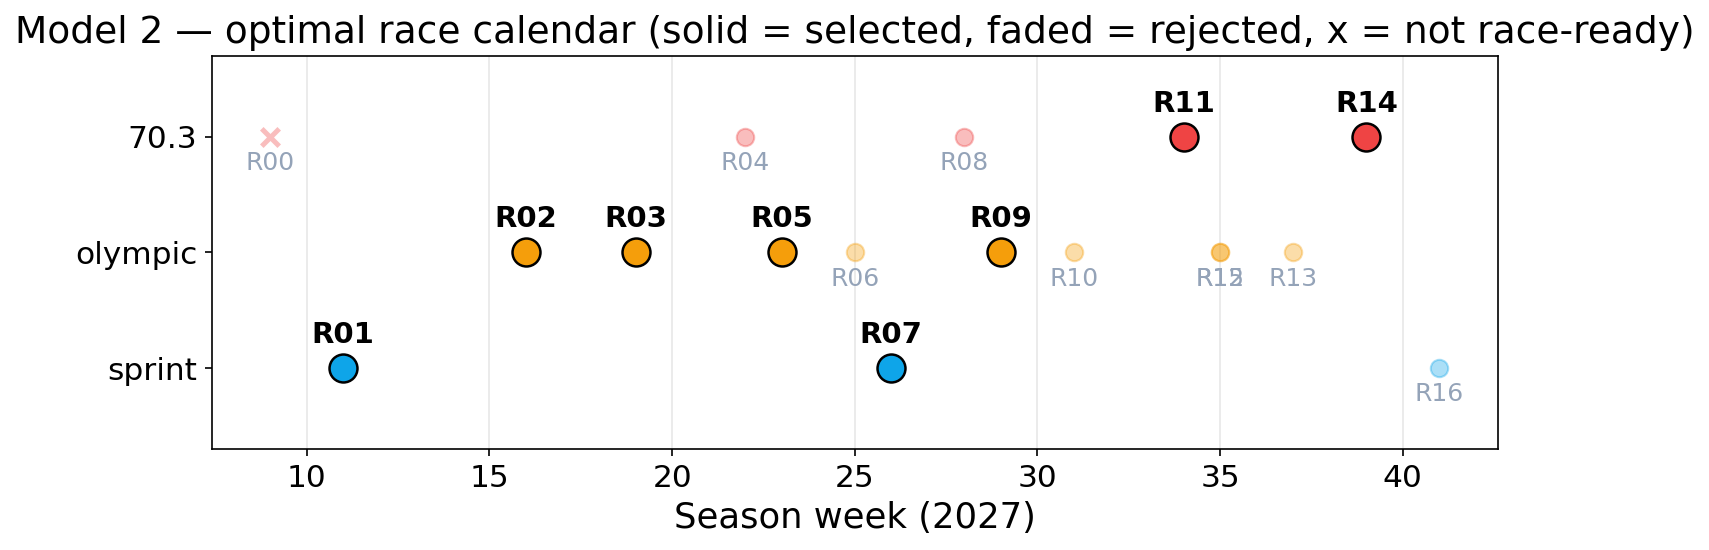
\includegraphics[width=.78\textwidth]{model2_calendar.png}
\takeaway{8 of 17 races $\cdot$ value 571.7 $\cdot$ 2250/2500 EUR $\cdot$ 11/12 days}
\end{frame}

\note{\gr Οκτώ αγώνες από τους δεκαεπτά, συνολική αξία 571,7. Ξοδεύει 2250 από τα
2500 ευρώ και 11 από τις 12 ημέρες άδειας --- άρα και τα δύο σακίδια είναι σχεδόν
γεμάτα, αλλά κανένα δεν δεσμεύει ακριβώς, κάτι που θα έχει σημασία σε δύο
διαφάνειες.

Η ενδιαφέρουσα απόφαση είναι το φθινόπωρο. Το Πανελλήνιο Πρωτάθλημα και το 70.3
της περιοχής μου είναι αρκετά κοντά ώστε ο περιορισμός αποθεραπείας να απαγορεύει
και τα δύο. Ο optimizer κρατάει το 70.3.

Τα «χι» είναι αγώνες για τους οποίους δεν είμαι αρκετά έτοιμος· οι ξεθωριασμένοι
κύκλοι είναι αγώνες που θα μπορούσε να πληρώσει αλλά επέλεξε να μην τους
αγοράσει.}

\begin{frame}{Model 2 --- why Branch \& Bound is needed}
\begin{columns}
\column{.52\textwidth}
\centering
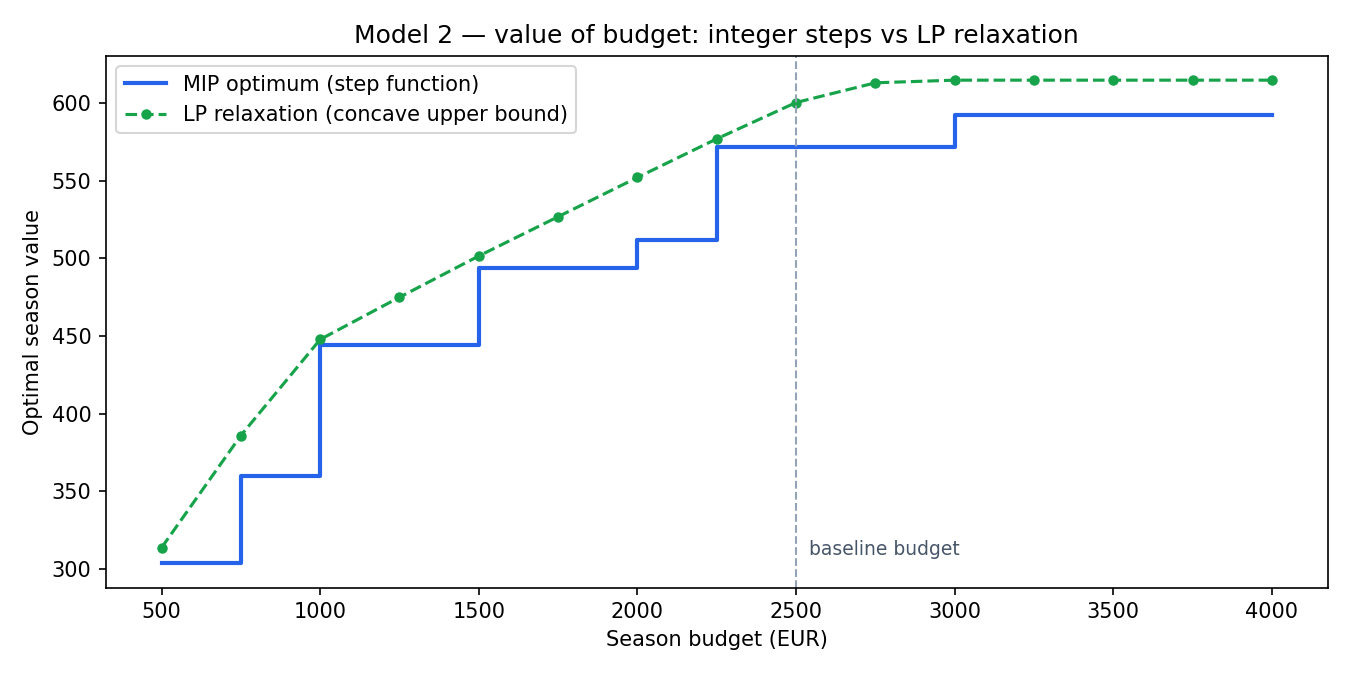
\includegraphics[width=\textwidth]{model2_budget_sweep.png}
\column{.46\textwidth}
\begin{itemize}\itemsep8pt
  \item LP $600.5$ vs.\ MIP $571.7$:\\ \textbf{integrality gap 5.0\%}
  \item 8 fractional variables; the champs/70.3 conflict splits \textbf{0.5/0.5}
  \item \textbf{clique cuts} (Bron--Kerbosch): $600.5 \to 591.0$,\\
        gap \textbf{5.04\% $\to$ 3.38\%}
\end{itemize}
\end{columns}
\end{frame}

\note{\gr Γιατί δεν λύνω απλώς τη γραμμική χαλάρωση και στρογγυλοποιώ; Επειδή η
χαλάρωση δίνει 600,5 έναντι πραγματικού βέλτιστου 571,7 --- κενό ακεραιότητας 5
τοις εκατό --- και οκτώ μεταβλητές βγαίνουν κλασματικές. Η σύγκρουση Πρωτάθλημα
εναντίον 70.3 που μόλις περιέγραψα σπάει ακριβώς μισό-μισό: η χαλάρωση παίρνει
μισό από κάθε αγώνα, που δεν σημαίνει τίποτα. Χρειάζεται Branch and Bound.

Το σχήμα είναι η αξία του χρήματος. Το βέλτιστο του MIP είναι κλιμακωτή
συνάρτηση --- οι αγώνες κοστίζουν όσο κοστίζουν, οπότε τα επιπλέον ευρώ δεν
κάνουν τίποτα μέχρι να φτάσουν να πληρώσουν άλλη μία συμμετοχή --- και βρίσκεται
κάτω από την κοίλη καμπύλη της χαλάρωσης. Πάνω από τα 3000 ευρώ τα σκαλοπάτια
σταματούν, γιατί ο δεσμευτικός πόρος αλλάζει από χρήματα σε ημέρες άδειας.

Για τα cutting planes: φτιάχνω τον γράφο συγκρούσεων των περιορισμών αποθεραπείας
και τρέχω Bron--Kerbosch για να βρω τις μέγιστες κλίκες του. Κάθε κλίκα μεγέθους
τρία ή παραπάνω δίνει μια έγκυρη ανισότητα, άθροισμα των x της κλίκας το πολύ
ένα, που κυριαρχεί των ανά ζεύγος περιορισμών. Τέσσερις τέτοιες τομές σφίγγουν τη
χαλάρωση από 600,5 σε 591, κλείνοντας το ένα τρίτο του κενού, και δεν αποκόπτουν
κανένα ακέραιο σημείο --- το βέλτιστο μένει αμετάβλητο.}

\begin{frame}{Model 2 --- the dual problem}
\[
\kappa_i y_\mathcal{B} + \delta_i y_\mathcal{D} + y_{\text{month}(i)}
+ \sum_{j} y_{ij} - [i \in A] y_A \;\ge\; v_i
\]
\begin{center}\small
\emph{a race enters only if its value covers the shadow cost of what it consumes}
\end{center}
\vspace{4pt}
\begin{center}\small
\begin{tabular}{llr}
\toprule
Dual & Meaning & Price\\
\midrule
$y_{13,14}$ & Champs vs.\ Costa Navarino conflict & \textbf{56.40}\\
$y_{06,07}$ & Hamburg vs.\ Thessaloniki conflict & 31.67\\
$y_\mathcal{B}$ & one extra euro & 0.094\\
$y_\mathcal{D}$ & one extra vacation day & $\approx 0$\\
\bottomrule
\end{tabular}
\end{center}
\takeaway{The scarce resource is calendar space --- not money.}
\end{frame}

\note{\gr Η γραμμική χαλάρωση είναι ήδη σε τυπική μορφή, max c-ανάστροφο-x υπό Ax
μικρότερο ή ίσο του b με x μη αρνητικό, οπότε το δυϊκό είναι το σχολικό: min
b-ανάστροφο-y με A-ανάστροφο-y μεγαλύτερο ή ίσο του c. Γράφοντας μία δυϊκή γραμμή
παίρνω την ανισότητα της διαφάνειας, και έχει καθαρή ανάγνωση: ένας αγώνας μπαίνει
στο ημερολόγιο μόνο αν η αξία του καλύπτει το σκιώδες κόστος όλων όσων καταναλώνει
--- budget, ημέρες άδειας, τη θέση του μήνα του, και κάθε σύγκρουση στην οποία
συμμετέχει.

Τώρα διαβάστε τις τιμές. Ένα ευρώ αξίζει 0,094. Μία ημέρα άδειας ουσιαστικά
μηδέν. Αλλά η σύγκρουση αποθεραπείας ανάμεσα στο Πρωτάθλημα και στην Costa
Navarino τιμολογείται στο 56,4 --- τρεις τάξεις μεγέθους πάνω από το ευρώ.

Άρα η διαίσθηση με την οποία ξεκίνησα ήταν λάθος. Υπέθετα ότι ο περιορισμός ήταν
τα χρήματα. Το δυϊκό λέει ότι ο σπάνιος πόρος είναι ο χώρος στο ημερολόγιο: οι
εβδομάδες αποθεραπείας μεταξύ αγώνων. Πρακτικά, το να διαπραγματευτώ ημερομηνίες
αξίζει πολύ περισσότερο από το να βρω χορηγία.}

\begin{frame}{Model 2 --- network-flow extension}
Drop the knapsacks and the monthly cap $\Rightarrow$ only recovery spacing remains:
\begin{center}
\textbf{feasible calendars $=$ paths in a DAG}
\end{center}
\vspace{6pt}
Three methods, identical answer $z = 639.4$:
\begin{enumerate}\itemsep4pt
  \item dynamic programming --- longest path in topological order
  \item \textbf{flow LP, continuous variables --- integral anyway}
  \item restricted 0--1 MIP
\end{enumerate}
\takeaway{Totally unimodular. The knapsacks are what break the structure.}
\end{frame}

\note{\gr Αυτή η διαφάνεια συνδέει την εργασία με το κομμάτι των δικτύων της ύλης.

Αν αφαιρέσω τα δύο σακίδια και το μηνιαίο πλαφόν, και κρατήσω μόνο την
αποθεραπεία, το πρόβλημα αλλάζει τελείως χαρακτήρα. Βάζω τους αγώνες ως κόμβους
σε σειρά εβδομάδας και τραβάω ακμή από τον i στον j όταν το κενό είναι
τουλάχιστον όσο η αποθεραπεία που απαιτεί ο i. Τότε ένα εφικτό ημερολόγιο είναι
ακριβώς μια διαδρομή σε αυτό το κατευθυνόμενο άκυκλο γράφημα, και το καλύτερο
ημερολόγιο είναι η μακρύτερη διαδρομή.

Το έλυσα με τρεις τρόπους και πήρα 639,4 και τις τρεις φορές. Ο μεσαίος είναι το
θεωρητικό σημείο: το έλυσα ως LP ροής με συνεχείς μεταβλητές, χωρίς κανέναν
περιορισμό ακεραιότητας, και η λύση βγήκε ακέραια από μόνη της. Αυτό είναι ολική
μονοπαραγοντικότητα --- ο πίνακας πρόσπτωσης κόμβων-ακμών είναι TU, άρα κάθε
βασική εφικτή λύση είναι ακέραια και κάθε βάση αντιστοιχεί σε ένα συνδετικό
δέντρο. Αυτή ακριβώς είναι η δομή που εκμεταλλεύεται ο Network Simplex. Δεκαοκτώ
κόμβοι, 136 ακμές.

Και αυτό λέει κάτι για το πλήρες μοντέλο: είναι οι περιορισμοί σακιδίου, το
budget και οι ημέρες άδειας, που καταστρέφουν τη δομή δικτύου και επιβάλλουν
Branch and Bound. Χωρίς αυτούς, δεν χρειάζεται καθόλου διακλάδωση.}

% ---------------------------------------------------------------- model 3
\begin{frame}{Model 3 --- race pacing (LP with linearization)}
\textbf{Variables} \quad minutes $t_{\ell z}$: 3 legs $\times$ 5 zones $= 15$
\vspace{4pt}

\textbf{Linearization} \quad within a zone, speed and energy rate are \emph{constants}
\[
\min \sum_{\ell,z} t_{\ell z} + T_1 + T_2
\quad \text{s.t.} \quad
\underbrace{\textstyle\sum_z s_{\ell z} t_{\ell z} \ge d_\ell}_{\text{distances}},\;
\underbrace{\textstyle\sum e_{\ell z} t_{\ell z} \le k_E \cdot \text{CTL}_T}_{\text{energy budget (Model 1)}},\;
\underbrace{\text{Z4+ caps}}_{\text{per leg}},\;
\underbrace{\varphi \cdot G}_{\text{bike} \to \text{run}}
\]
\vspace{-6pt}
\begin{center}\small
bike speed $\propto \phi(\gamma)\cdot(\text{power})^{1/3}$ \quad --- \quad
$\phi(\gamma)$ from the power balance, \textbf{derived, not fitted}
\end{center}
\end{frame}

\note{\gr Εδώ η φυσική είναι μη γραμμική: η σχέση ταχύτητας και ενεργειακού
κόστους είναι καμπύλη, όχι ευθεία. Το κόλπο είναι να διακριτοποιήσω την ένταση
στις πέντε προπονητικές ζώνες. Μέσα σε μια ζώνη, η ταχύτητα και ο ρυθμός
κατανάλωσης είναι σταθερές, άρα και η απόσταση και η ενέργεια γίνονται γραμμικές
ως προς τον χρόνο που ξοδεύω εκεί, και το πρόβλημα ξαναγίνεται LP. Δεκαπέντε
μεταβλητές. Αυτή είναι η κλασική κατά τμήματα γραμμική προσέγγιση του μαθήματος,
και οι ζώνες δεν είναι αυθαίρετες --- είναι οι ζώνες στις οποίες προπονούνται
πραγματικά οι αθλητές.

Δύο όροι αξίζουν κουβέντα. Η ταχύτητα στο ποδήλατο πάει με την κυβική ρίζα της
ισχύος, επειδή η αεροδυναμική αντίσταση πάει με την ταχύτητα στον κύβο --- αν
διπλασιάσεις την ισχύ σου δεν πλησιάζεις καν τον διπλασιασμό της ταχύτητας.

Και το φι του γάμμα είναι ο συντελεστής κλίσης της διαδρομής. Μοντελοποιώ μια
διαδρομή που ανεβαίνει γάμμα μέτρα ανά χιλιόμετρο ως μισή ανηφόρα και μισή
κατηφόρα με σταθερή ισχύ, και παίρνω τον αρμονικό μέσο των δύο ταχυτήτων. Η
αεροδυναμική σταθερά προκύπτει αντίστροφα από τη δική μου ταχύτητα σε επίπεδη
διαδρομή, οπότε τίποτα μέσα στο φι δεν είναι προσαρμοσμένο σε αποτέλεσμα αγώνα.
Αυτό θα έχει σημασία στην επικύρωση, τρεις διαφάνειες πιο κάτω.

Ο τελευταίος όρος είναι η σύζευξη που κάνει το πρόβλημα τρίαθλο και όχι τρεις
ξεχωριστούς αγώνες: κάθε κιλοτζάουλ σκληρής δουλειάς στο ποδήλατο μειώνει το πόσο
μακριά μπορώ μετά να τρέξω.}

\begin{frame}{Model 3 --- ``steady bike, hard run,'' derived}
\centering
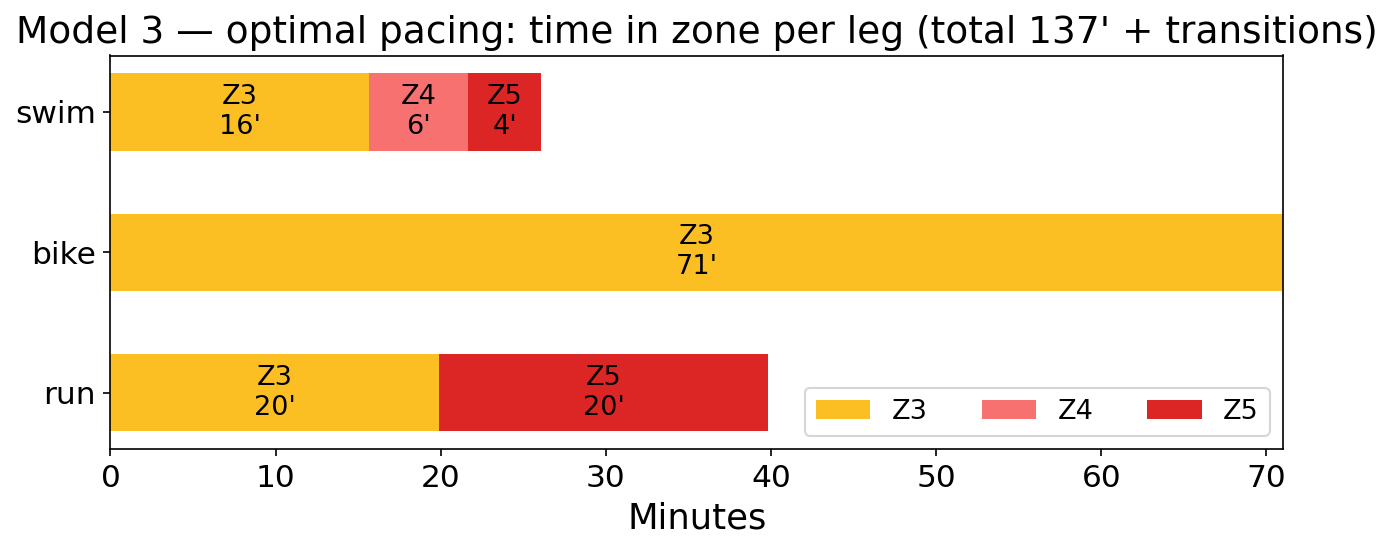
\includegraphics[width=.70\textwidth]{model3_pacing.png}
\takeaway{Bike entirely Z3. Energy budget exhausted \emph{exactly}: 9389 kJ.}
\end{frame}

\note{\gr Ολυμπιακή απόσταση σε 140,4 λεπτά, και το ενεργειακό budget εξαντλείται
ακριβώς --- 9389 κιλοτζάουλ διαθέσιμα, 9389 καταναλωμένα. Ο ενεργειακός
περιορισμός είναι δεσμευτικός, γι' αυτό και η δυϊκή του τιμή είναι το ενδιαφέρον
νούμερο της επόμενης διαφάνειας.

Η δομή της απάντησης είναι το προπονητικό κλισέ «σταθερό ποδήλατο, δυνατό
τρέξιμο», και το LP το βγάζει χωρίς να του το πει κανείς. Το ποδήλατο είναι
εξ ολοκλήρου στη ζώνη 3, τίποτα πιο σκληρό. Γιατί; Για δύο λόγους, και οι δύο
μέσα στο μοντέλο: η κυβική ρίζα σημαίνει ότι το σκληρό ποδήλατο αγοράζει ελάχιστη
ταχύτητα, και ο όρος σύζευξης σημαίνει ότι σου κοστίζει άμεσα απόσταση στο
τρέξιμο. Οπότε ο optimizer ξοδεύει την ένταση εκεί που η ένταση είναι φθηνή,
δηλαδή στο τρέξιμο.}

\begin{frame}{Model 3 --- what is a watt worth?}
\centering
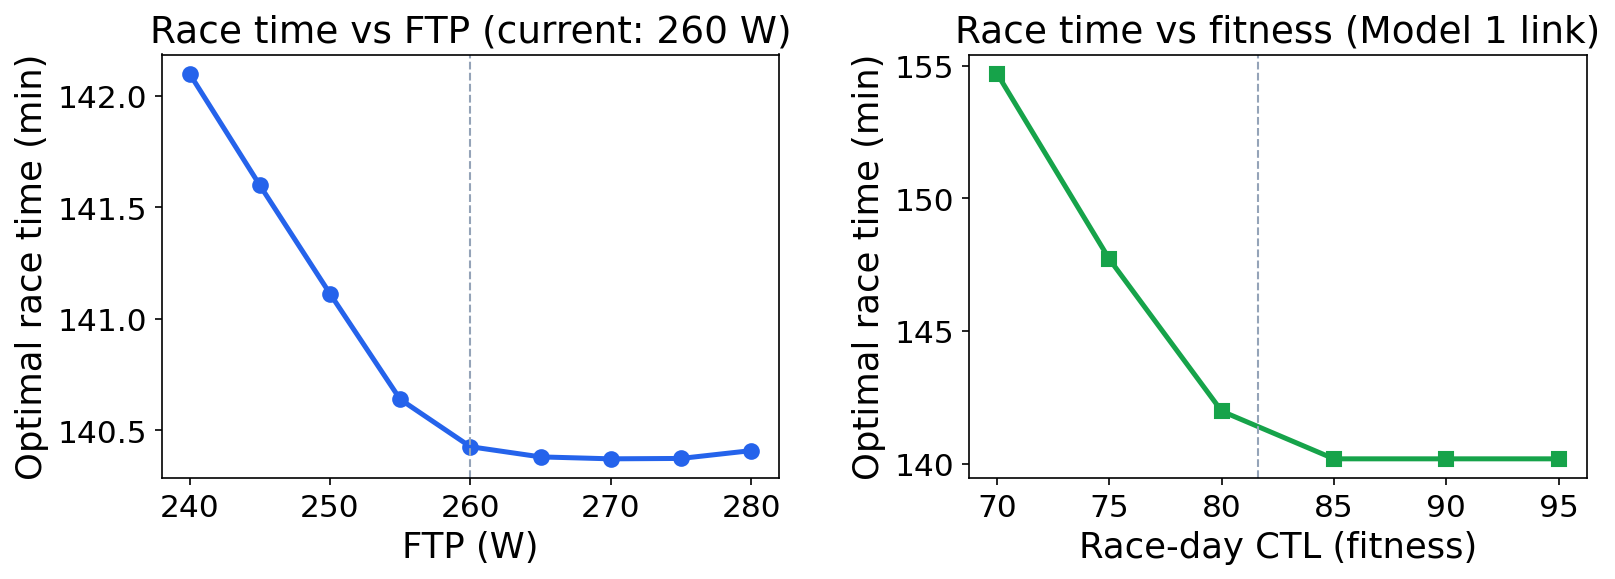
\includegraphics[width=.86\textwidth]{model3_sweeps.png}
\takeaway{$+1$ CTL $=$ 69--84 s. $+1$ W $\approx$ 6 s --- but only below 260 W.}
\end{frame}

\note{\gr Δύο σαρώσεις ευαισθησίας, και οι δύο απαντούν σε ερωτήματα που κάνει
ένας πραγματικός αθλητής.

Αριστερά: τι αξίζει ένα βατ; Κάτω από τα 260 βατ, κάθε επιπλέον βατ threshold
ισχύος αξίζει περίπου έξι δευτερόλεπτα. Πάνω από εκεί, η αξία καταρρέει στο μηδέν.
Αυτό δεν είναι σφάλμα --- είναι ο ενεργειακός περιορισμός. Με σταθερό απόθεμα
κιλοτζάουλ, δεν έχει νόημα να μπορείς να παράγεις περισσότερη ισχύ, γιατί δεν
μπορείς να την τροφοδοτήσεις. Το σκέλος του ποδηλάτου γίνεται ενεργειακά
περιορισμένο αντί για περιορισμένο από ισχύ.

Δεξιά: τι αξίζει μία μονάδα φόρμας; Εξήντα εννιά έως ογδόντα τέσσερα δευτερόλεπτα
ανά μονάδα CTL, και κρατάει μέχρι περίπου CTL 85.

Άρα τα δύο νούμερα μαζί δίνουν ξεκάθαρο προπονητικό συμπέρασμα: χτίσε αντοχή, όχι
μέγιστη ισχύ. Και αυτό βγήκε από σκιώδη τιμή, όχι από γνώμη. Η ίδια η δυϊκή τιμή
της ενέργειας, παρεμπιπτόντως, είναι 0,43 δευτερόλεπτα ανά κιλοτζάουλ.}

\begin{frame}{Model 3 --- validated against three real races}
\begin{center}\small
\begin{tabular}{llrrrrrr}
\toprule
& & \multicolumn{2}{c}{Swim} & \multicolumn{2}{c}{Bike} & \multicolumn{2}{c}{Run}\\
Race & CTL & mdl & act & mdl & act & mdl & act\\
\midrule
Spetsathlon '26 (sprint$^\ast$) & 64.9 & 12.9 & 13.2 & 47.3 & 50.9 & 18.7 & 17.7\\
Epidavros '25 (Olympic) & 55.6 & 27.2 & 25.8 & 88.8 & 91.5 & 38.9 & 42.0\\
70.3 Costa Navarino '25 & 71.4 & 33.3 & 32.9 & 184.6 & 180.3 & 86.4 & \textbf{115.2}\\
\bottomrule
\end{tabular}

{\scriptsize minutes $\cdot$ $^\ast$non-standard 25 km bike}
\end{center}
\vspace{4pt}
\begin{itemize}\itemsep5pt
  \item swim within 0.5 min every time
  \item binding constraint \textbf{switches with distance}: speed caps $\to$ energy
        $\to$ infeasible unfed
  \item the 70.3 run: my \textbf{29-minute} wall is the energy constraint, violated in real life
\end{itemize}
\end{frame}

\note{\gr Αυτό είναι το κομμάτι που δεν θα μπορούσα να κάνω με πλασματικά
δεδομένα. Βρήκα τις τρεις ημέρες αγώνα μέσα στο ακατέργαστο export --- είναι οι
μόνες τρεις μέρες που περιέχουν κολύμπι, ποδήλατο και τρέξιμο --- και πήρα την
κατάσταση φόρμας από την αλυσίδα επεξεργασίας, από την προηγούμενη μέρα. Τίποτα
εδώ δεν ρυθμίστηκε για να δείχνουν ωραία τα νούμερα.

Το κολύμπι πέφτει μέσα σε μισό λεπτό και τις τρεις φορές, που μου λέει ότι τα
μετρημένα κατώφλια είναι σωστά.

Η επιστημονικά ενδιαφέρουσα γραμμή είναι η μεσαία: το ποιος περιορισμός δεσμεύει
αλλάζει με την απόσταση του αγώνα. Στο sprint είναι τα πλαφόν ταχύτητας των
ζωνών --- με περιορίζει η τελική ταχύτητα, όχι το καύσιμο. Στην ολυμπιακή είναι η
ενέργεια. Στο 70.3 το μοντέλο βγαίνει εντελώς ανέφικτο με μόνο την αποθηκευμένη
ενέργεια· λύνεται μόνο αν το ταΐσεις. Και η πρόσληψη που χρειάζεται είναι περίπου
21 κιλοτζάουλ το λεπτό, που μεταφράζεται σε 75 γραμμάρια υδατανθράκων την ώρα ---
την τυπική οδηγία της αθλητικής διατροφής, ανακτημένη από ένα γραμμικό πρόγραμμα
που δεν την είχε ακούσει ποτέ.

Και τώρα η τίμια αποτυχία. Το μοντέλο προβλέπει 86 λεπτά για το τρέξιμο του 70.3·
εγώ έκανα 115. Αλλά δείτε τι συνέβη: μετά το δέκατο χιλιόμετρο πήγα από 4:53 ανά
χιλιόμετρο σε 5:52, με τον παλμό να πέφτει από 162 σε 145. Το να επιβραδύνεις ενώ
ο παλμός σου πέφτει δεν είναι κακή διαχείριση ρυθμού, είναι να σου τελειώνει το
καύσιμο. Άρα αυτά τα 29 λεπτά δεν είναι λάθος του μοντέλου --- είναι εγώ που
παραβίασα τον ενεργειακό περιορισμό στην πραγματικότητα. Το μοντέλο μου λέει πόσο
μου κόστισε.}

\begin{frame}{What the bike residual is made of}
\begin{center}\small
\begin{tabular}{lrrrrr}
\toprule
Bike leg & m/km & no gradient & $\phi(\gamma)$ & 2-param fit & actual\\
\midrule
Spetsathlon (24.4 km) & 15.2 & 43.3 & \textbf{47.3} & 55.0 & 50.9\\
Epidavros (38.7 km) & 15.5 & 78.9 & \textbf{88.8} & 87.7 & 91.5\\
Costa Navarino (88.5 km) & 9.1 & 177.5 & \textbf{184.6} & 180.0 & 180.3\\
\midrule
\multicolumn{2}{l}{total error} & 23.0 min & \textbf{10.6 min} & 8.2 min & \\
\multicolumn{2}{l}{parameters fitted here} & 0 & \textbf{0} & 2 & \\
\bottomrule
\end{tabular}
\end{center}
\vspace{6pt}
\begin{itemize}\itemsep5pt
  \item no gradient $\Rightarrow$ too fast on \textbf{every} course: a missing term, not noise
  \item $\phi(\gamma)$ from physics halves the error with \textbf{zero} fitted parameters
\end{itemize}
\end{frame}

\note{\gr Το ποδήλατο είναι το λιγότερο ακριβές σκέλος, οπότε θέλω να δείξω ότι
ξέρω γιατί, αντί να ελπίζω ότι δεν θα ρωτήσει κανείς.

Το ερώτημα: το υπόλοιπο του ποδηλάτου είναι απλώς θόρυβος, ή λείπει όρος από το
μοντέλο; Δύο στοιχεία λένε ότι λείπει όρος. Πρώτον το μέγεθος --- 23 λεπτά σε
τρεις αγώνες. Δεύτερον, και πιο αποκαλυπτικό, το πρόσημο: αν προσποιηθώ ότι κάθε
διαδρομή είναι επίπεδη, βγαίνω γρηγορότερος και στις τρεις. Ο θόρυβος δεν έχει
πρόσημο.

Ο όρος που λείπει είναι η κλίση, και επίτηδες δεν την κόλλησα εκ των υστέρων.
Ανήκει στη διατύπωση, οπότε το φι του γάμμα είναι μέρος του μοντέλου, παραγόμενο
από το ισοζύγιο ισχύος του ποδηλάτου, με μηδέν παραμέτρους προσαρμοσμένες σε
αυτούς τους αγώνες. Αυτό είναι γνήσιο out-of-sample τεστ και υποδιπλασιάζει το
σφάλμα στα 10,6 λεπτά, με τα υπόλοιπα να πέφτουν πλέον και από τις δύο πλευρές
του μηδενός.

Η τελευταία στήλη είναι ο έλεγχός μου. Προσάρμοσα και μια εμπειρική διόρθωση δύο
παραμέτρων κατευθείαν πάνω σε αυτούς τους τρεις αγώνες --- που είναι ζαβολιά, και
αποτελεί άνω φράγμα του πόσο καλή θα μπορούσε να φανεί οποιαδήποτε τέτοια
διόρθωση. Κερδίζει μόλις 2,4 λεπτά παραπάνω. Άρα η κλίση εξηγεί ουσιαστικά όλο το
ανακτήσιμο σφάλμα, και η παραγόμενη εκδοχή το παίρνει σχεδόν όλο δωρεάν.

Και η μικρή μεροληψία που απομένει εξηγείται κι αυτή: το φι υποθέτει ότι κρατάω
threshold ισχύ στις κατηφόρες, που δεν το κάνει κανείς, οπότε μένω ελαφρώς
αισιόδοξος στις δύο ανηφορικές διαδρομές.}

% ---------------------------------------------------------------- playing with the model
\begin{frame}{Sensitivity across sizes and parameters}
\begin{columns}
\column{.52\textwidth}
\centering
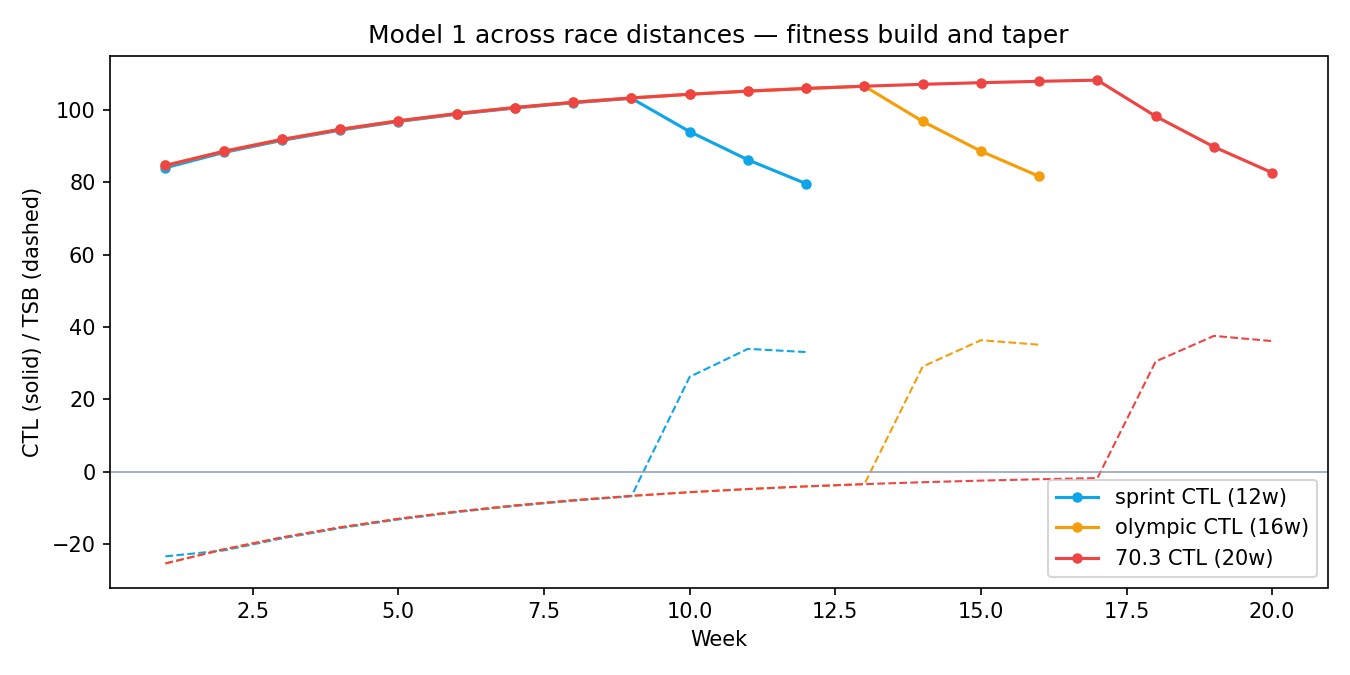
\includegraphics[width=\textwidth]{model1_distance_scenarios.png}
\column{.46\textwidth}
\begin{itemize}\itemsep10pt
  \item \textbf{Sizes:} 12/16/20 weeks, 144--240 vars --- structure invariant
  \item \textbf{$k_2 \in [1,3]$:} race-day TSB stays $35 \pm 2$
  \item \textbf{Cost ranging:} plan invariant for $k_1 \in [0.68, 1.56]$,
        $k_2 \in [1.29, 2.95]$
  \item \textbf{Solve times:} all $< 10$ ms
\end{itemize}
\end{columns}
\end{frame}

\note{\gr Η εκφώνηση ζητάει να «παίξουμε» με το μοντέλο, οπότε: τρία είδη
διαταραχής.

Μέγεθος. Ξανάτρεξα τον μακρόκυκλο σε 12, 16 και 20 εβδομάδες --- από 144 μέχρι
240 μεταβλητές. Οι μεγαλύτεροι ορίζοντες βοηθούν, η αντικειμενική πάει από μείον
13,5 σε μείον 10,4, με φθίνουσες αποδόσεις, και η δομή χτίσιμο-και-μετά-taper
είναι πανομοιότυπη και στις τρεις. Δηλαδή η ποιοτική απάντηση δεν εξαρτάται από
τον ορίζοντα που έτυχε να διαλέξω.

Βαθμονόμηση της αντικειμενικής. Το k2 είναι η παράμετρος για την οποία είμαι πιο
ανασφαλής, οπότε το σάρωσα από 1 έως 3: η φόρμα την ημέρα του αγώνα μετακινείται
ελάχιστα, 35 συν πλην 2. Το βάθος του taper το καθορίζουν οι περιορισμοί --- τα
ελάχιστα της εβδομάδας αγώνα --- όχι η αντικειμενική, κάτι που με καθησυχάζει
επειδή τους περιορισμούς τους έχω μετρήσει.

Και τυπικό cost ranging, κατευθείαν από την ύλη: η βέλτιστη βάση επιβιώνει για k1
οπουδήποτε από 0,68 έως 1,56 και k2 από 1,29 έως 2,95. Τα δύο λιγότερο μετρήσιμα
νούμερα του μοντέλου μπορούν να μεταβληθούν κατά παράγοντα δύο χωρίς να αλλάξει
ούτε μία μεταβλητή.

Όλα λύνονται σε λιγότερο από δέκα χιλιοστά του δευτερολέπτου, οπότε τίποτα από
αυτά δεν μου κόστισε.}

\begin{frame}{Integrating the pipeline: coherence \& fixed point}
\textbf{Do the three objectives agree?}
\begin{itemize}\itemsep5pt
  \item $E = k_E\text{CTL}$ ignores fatigue $\Rightarrow$ four different plans,
        \textbf{same 140.2 min}
  \item $E = E_0 + k_E(\text{CTL}_T - \lambda\,\text{ATL}_T)$ is affine in $p_T$
        \textbf{iff} $\lambda = k_2/k_1$
  \item $E > 0$ needs $\lambda < 1.75$, so $k_2 = 2$ is \emph{incoherent};
        cost ranging licenses $\lambda = 1.5$ --- \textbf{changing no variable}
\end{itemize}
\vspace{6pt}
\textbf{Which model comes first?} Iterate.
\begin{center}\small
\begin{tabular}{clrlr}
\toprule
Iter. & Macrocycle & Weeks & Selected A-race & Outcome\\
\midrule
1 & olympic & 16 & R14 Costa Navarino (70.3) & re-plan as 70.3\\
2 & 70.3 & 20 & R14 Costa Navarino (70.3) & \textbf{fixed point}\\
\bottomrule
\end{tabular}
\end{center}
\end{frame}

\note{\gr Δύο προβλήματα ολοκλήρωσης, που τα θεωρώ το πιο ενδιαφέρον κομμάτι της
εργασίας, επειδή και τα δύο ανακαλύφθηκαν με έλεγχο και όχι με υπόθεση.

Πρώτον, η συνέπεια. Το Μοντέλο 1 μεγιστοποιεί έναν δείκτη απόδοσης· το Μοντέλο 3
ελαχιστοποιεί χρόνο αγώνα. Συμφωνούν; Το δοκίμασα: παρήγαγα τέσσερα αρκετά
διαφορετικά προπονητικά πλάνα και τα έδωσα στο Μοντέλο 3, και τα τέσσερα έδωσαν
τα ίδια 140,2 λεπτά. Το Μοντέλο 3 ήταν τυφλό στην προπόνηση --- επειδή το
ενεργειακό budget ήταν k-E επί CTL, που αγνοεί τελείως την κόπωση. Μπορούσες να
κάνεις taper ή να μην κάνεις και ο αγώνας έβγαινε ίδιος. Αυτό είναι σπασμένη
αλυσίδα.

Η διόρθωση είναι ένα μικρό θεώρημα. Κάνε το budget να εξαρτάται από τη φόρμα:
E-μηδέν συν k-E επί CTL μείον λάμδα επί ATL. Τότε το budget είναι γνησίως αύξουσα
αφινική συνάρτηση της αντικειμενικής του Μοντέλου 1 ακριβώς όταν το λάμδα ισούται
με k2 προς k1 --- και σε αυτή την περίπτωση η μεγιστοποίηση της απόδοσης είναι
αποδεδειγμένα το ίδιο με την ελαχιστοποίηση του χρόνου. Τα μοντέλα
ευθυγραμμίζονται εξ ορισμού, όχι στην τύχη.

Υπάρχει όμως μια παγίδα, και είναι ωραία. Το budget πρέπει να μένει θετικό, που
απαιτεί λάμδα μικρότερο από CTL προς ATL, δηλαδή 1,75. Το k2 που είχα υποθέσει
ίσο με 2 δίνει λάμδα 2 --- ασυνεπές. Άρα το θεώρημα δεν ευθυγραμμίζει απλώς τα
μοντέλα, απορρίπτει μια παράμετρο που είχα διαλέξει. Και εδώ αποδίδει το cost
ranging της προηγούμενης διαφάνειας: λέει ότι το k2 οπουδήποτε από 1,29 έως 2,95
αφήνει το πλάνο αμετάβλητο. Οπότε βάζω λάμδα 1,5, η αλυσίδα γίνεται συνεπής, και
δεν κουνιέται ούτε μία από τις 144 μεταβλητές.

Δεύτερον, η κυκλικότητα. Ο αγώνας-στόχος ορίζει το μήκος του μακρόκυκλου για το
Μοντέλο 1, αλλά το Μοντέλο 1 τροφοδοτεί την πύλη ετοιμότητας του Μοντέλου 2 που
επιλέγει τον αγώνα-στόχο. Αντί να υποθέσω σειρά, έκανα επανάληψη μέχρι σταθερό
σημείο --- δύο επαναλήψεις. Και η επανάληψη βρήκε πραγματικό λάθος: είχα υποθέσει
16 εβδομάδες για ολυμπιακή, αλλά ο αγώνας-στόχος που επιλέγει το ημερολόγιο είναι
70.3, που θέλει 20 εβδομάδες. Αν είχα υποθέσει σειρά, αυτό θα έμενε κρυφό.}

% ---------------------------------------------------------------- payoff
\begin{frame}{What the models actually recommend}
\begin{itemize}\itemsep9pt
  \item \textbf{Train more, much easier.} 6.6 h/wk at 37\% hard
        $\rightarrow$ 9.0 h/wk at \textbf{15\%}
  \item \textbf{More hours are worthless} above 10.5 h/wk --- recovery is what binds
  \item \textbf{Build endurance, not watts.} $+1$ CTL $=$ 69--84 s; $+1$ W $\approx 0$ above 260 W
  \item \textbf{Ride Z3, run hard, fuel 75 g/h.} The 70.3 positive split cost 29 min
  \item \textbf{Protect the calendar, not the budget.} Conflict dual 56.4 vs.\ 0.094/EUR
\end{itemize}
\end{frame}

\note{\gr Αν πάρω στα σοβαρά τη δική μου εργασία, να τι αλλάζει από τη Δευτέρα.

Η πρώτη γραμμή είναι αυτή που πονάει. Αυτή τη στιγμή προπονούμαι 6,6 ώρες την
εβδομάδα με το 37 τοις εκατό σκληρό. Το μοντέλο λέει 9 ώρες με 15 τοις εκατό
σκληρό. Είμαι αντι-πολωμένος --- προπονούμαι πολύ λίγο και πολύ δυνατά. Είναι η
μία αλλαγή με τη μεγαλύτερη απόδοση, και δεν θα την πίστευα χωρίς τις σκιώδεις
τιμές.

Δεύτερον, πρέπει να σταματήσω να ψάχνω κι άλλες ώρες προπόνησης πάνω από τις
δέκα μισή· αξίζουν κυριολεκτικά μηδέν. Ο δεσμευτικός πόρος είναι η ικανότητα
αποκατάστασης.

Τρίτον, από τη σάρωση των βατ: δουλειά αντοχής, όχι threshold ισχύς.

Τέταρτον, εκτέλεση αγώνα: ποδήλατο στη ζώνη 3, κράτα το για το τρέξιμο, σταθερός
ρυθμός, και 75 γραμμάρια υδατανθράκων την ώρα. Το θετικό σπλιτ μου στο 70.3
κόστισε 29 λεπτά.

Πέμπτον, διαπραγματεύσου ημερομηνίες αντί να κυνηγάς χρήματα --- 56,4 έναντι
0,094.

Και μία διόρθωση σχεδιασμού που την αποκάλυψε μόνο η επανάληψη σταθερού σημείου:
παράλειψε το Ντουμπάι στην αρχή της σεζόν γιατί δεν θα προλάβω να είμαι έτοιμος,
και αν ο αγώνας-στόχος είναι 70.3, χτίσε 20 εβδομάδες, όχι 16.}

\begin{frame}{Conclusions}
\begin{itemize}\itemsep10pt
  \item Three coupled models on \textbf{real personal data}
  \item Spanning the syllabus: LP \& Simplex, duality \& sensitivity,
        IP \& Branch \& Bound, network flows \& total unimodularity
  \item The optimizer \textbf{re-derives coaching wisdom} --- periodization,
        polarization, ``steady bike, hard run''
  \item Duals name the real bottlenecks: \emph{recovery}, \emph{calendar space},
        \emph{endurance}
  \item Reproducible: \texttt{python -m src.run\_all}, 60 tests
\end{itemize}
\vspace{6pt}
\begin{center}
{\footnotesize\url{https://github.com/manos1503/triathlon-optimization}}

\vspace{6pt}
\Large Thank you --- questions?
\end{center}
\end{frame}

\note{\gr Κλείνοντας. Τρία συζευγμένα μοντέλα, χτισμένα πάνω σε πραγματικά
προσωπικά δεδομένα και όχι σε σχολικό παράδειγμα, και μαζί καλύπτουν ουσιαστικά
όλη την ύλη: LP και Simplex, δυϊκότητα και ανάλυση ευαισθησίας, ακέραιο
προγραμματισμό με Branch and Bound και τομές, και δίκτυα ροής με ολική
μονοπαραγοντικότητα.

Δύο πράγματα που δεν τα περίμενα όταν ξεκίνησα. Ο optimizer ξαναβγάζει
προπονητική γνώση που δεν του την είπε κανείς --- περιοδικότητα, πολωμένη ένταση,
σταθερό ποδήλατο και δυνατό τρέξιμο. Και οι δυϊκές τιμές διέψευσαν συστηματικά τη
διαίσθησή μου για το τι με περιορίζει: όχι ο χρόνος, όχι τα χρήματα, αλλά η
ικανότητα αποκατάστασης, ο χώρος στο ημερολόγιο, και η αντοχή.

Όλα τρέχουν με μία εντολή και καλύπτονται από 60 tests. Σας ευχαριστώ --- είμαι
στη διάθεσή σας για ερωτήσεις.}

% ---------------------------------------------------------------- backup
\appendix
\begin{frame}{Backup: limitations}
\begin{itemize}\itemsep8pt
  \item \textbf{Weekly} time step for the Banister dynamics
  \item \textbf{Sequential} pipeline, not joint optimization
  \item \textbf{Constructed parameters} in Models 2--3 (race values, zone speeds, $k_E$)
  \item The LP's $+35$ TSB over-taper --- traced to race-week minimums
\end{itemize}
\end{frame}

\note{\gr Ημερήσια ανάλυση θα μετακινούσε τις σταθερές εξομάλυνσης αλλά όχι τη
δομή. Η από κοινού βελτιστοποίηση προπόνησης και ημερολογίου είναι φυσική και
αρκετά μεγαλύτερη επέκταση MIP --- αυτή είναι η προφανής συνέχεια. Οι
κατασκευασμένες παράμετροι είναι τεκμηριωμένες ως παραδοχές, και η ανάλυση
ευαισθησίας υπάρχει ακριβώς για να δείξει ποια συμπεράσματα επιβιώνουν όταν τις
διαταράξω. Και το υπερβολικό taper είναι τεχνούργημα περιορισμού, όχι εννοιολογικό
ελάττωμα του μοντέλου.}

\begin{frame}{Backup: alternative optima \& heuristic benchmark}
\textbf{Alternative optima:} fix $p_T = p^\ast$, re-solve min/max total hours
\begin{center}
same performance with \textbf{124.2 h} or \textbf{162.3 h} of season training
\end{center}
\vspace{8pt}
\textbf{vs.\ a standard coaching heuristic:}
\begin{itemize}\itemsep5pt
  \item violates the fatigue ceiling in \textbf{13 of 16 weeks}
  \item $p_T = -69.5$ vs.\ optimal $-11.4$
  \item but its race-day TSB $+21$ is inside the coaching band; the LP's $+35$ is not
\end{itemize}
\end{frame}

\note{\gr Ο εκφυλισμός γίνεται ορατός: καθηλώνω την αντικειμενική στη βέλτιστη
τιμή της και μετά ελαχιστοποιώ και μεγιστοποιώ τις συνολικές ώρες προπόνησης υπό
αυτόν τον περιορισμό. Και τα δύο είναι βέλτιστα πλάνα, και διαφέρουν κατά 38 ώρες
προπόνησης μέσα στη σεζόν. Αυτό είναι πραγματικό κενό αποδοτικότητας που η
αντικειμενική από μόνη της δεν το βλέπει.

Ο ευρετικός κανόνας είναι αυτό που θα έγραφε ένας λογικός προπονητής --- γέμισε
τις διαθέσιμες ώρες, 20/45/35 στα αθλήματα, 80/15/5 στις εντάσεις. Σπάει το ταβάνι
κόπωσης σε 13 από τις 16 εβδομάδες, που είναι χρόνια υπερπροπόνηση, και βαθμολογεί
πολύ χειρότερα. Δίκαια όμως, φέρνει τη φόρμα της ημέρας του αγώνα μέσα στην
αποδεκτή προπονητική ζώνη ενώ το δικό μου LP όχι --- που είναι ακριβώς το ερώτημα
ευαισθησίας του k2 από πριν.}

\end{document}
"
%       -> presentation-notes.pdf: the same slides with the Greek speaker notes
%          (xelatex, because the notes are in Greek and need a Unicode font)
%
% presentation-notes.pdf is a private rehearsal aid and is NOT committed.
%
% Design rule for this deck: the slide is the evidence, the speaker is the
% argument. Anything that is a sentence rather than a number, a name or a
% figure belongs in \note{}, not on screen.

\documentclass[10pt,aspectratio=169]{beamer}

\usetheme{Madrid}
\usecolortheme{seahorse}
\setbeamertemplate{navigation symbols}{}
\usepackage{amsmath,amssymb}
\usepackage{graphicx}
\usepackage{booktabs}

\ifdefined\shownotes
  \setbeameroption{show notes}
  \usepackage{fontspec}
  % Any installed font with Greek coverage; Helvetica ships with macOS.
  % Override on another machine, e.g. \def\notesfont{DejaVu Sans}
  \providecommand{\notesfont}{Helvetica}
  \newfontfamily\gr{\notesfont}
\else
  \providecommand{\gr}{}
\fi

\graphicspath{{../results/figures/}}

\definecolor{accent}{RGB}{30,60,140}
\setbeamercolor{frametitle}{fg=white,bg=accent}
\setbeamercolor{title}{fg=white,bg=accent}

% one-line takeaway strip under a figure
\newcommand{\takeaway}[1]{\vspace{2pt}\begin{center}\small\textbf{#1}\end{center}}

\title[Triathlon Optimization]{Optimal Resource Allocation and Scheduling\\
       of Athletic Activities, with an Application to Triathlon}
\subtitle{\normalsize Linear and 0--1 Integer Programming models for training
          load, race calendar and race pacing}
\author[E. Vichos]{Emmanouil Vichos (AM 1100830)}
\institute[UPatras]{Linear and Combinatorial Optimization --- University of Patras\\
                    Supervisor: Prof.\ S.\ Daskalaki}
\date{\today}

\begin{document}

\begin{frame}
\titlepage
\end{frame}

\note{\gr Καλημέρα σας. Η εργασία μου εφαρμόζει γραμμικό και ακέραιο
προγραμματισμό στο τρίαθλο --- και μάλιστα όχι σε πλασματικά δεδομένα: σε
δεκαπέντε μήνες δικής μου προπόνησης και σε τρεις αγώνες που πραγματικά έτρεξα.
Τρεις αποφάσεις, τρία μοντέλα, μία αλυσίδα.}

% ---------------------------------------------------------------- overview
\begin{frame}{Three decisions, one athlete}
\begin{enumerate}\itemsep8pt
  \item<1-> \textbf{How to train} --- hours per sport, per intensity, per week
  \item<2-> \textbf{Which races to enter} --- a season under money and recovery limits
  \item<3-> \textbf{How to race} --- spend a finite energy reserve over three legs
\end{enumerate}
\vspace{14pt}
\onslide<4->{
\begin{center}\large
\textbf{Model 1 (LP)} $\;\rightarrow\;$ \textbf{Model 2 (0--1 MIP)} $\;\rightarrow\;$ \textbf{Model 3 (LP)}\\[2pt]
\small training load \hfill race calendar \hfill pacing strategy
\end{center}}
\end{frame}

\note{\gr Οι τρεις αποφάσεις δεν είναι ανεξάρτητες, και αυτό ακριβώς είναι το
νόημα της εργασίας. Η φυσική κατάσταση χτίζεται αργά ενώ η κόπωση γρήγορα, οπότε
η προπόνηση είναι ένα δυναμικό trade-off σε ορίζοντα 12 έως 20 εβδομάδων.

Η κατάσταση φόρμας που βγάζει το Μοντέλο 1 κάνει μετά δύο πράγματα: καθορίζει σε
ποιους αγώνες είμαι έτοιμος να κατέβω, και ορίζει το ενεργειακό budget που έχω
διαθέσιμο την ημέρα του αγώνα. Άρα τα βέλη είναι πραγματικές συζεύξεις, όχι
αφηγηματικό στολίδι.}

% ---------------------------------------------------------------- data
\begin{frame}{Real data: 15 months of my own training}
\begin{columns}
\column{.55\textwidth}
\begin{itemize}\itemsep6pt
  \item Strava export: \textbf{598 activities}, 574 usable
  \item Banister training impulse per activity
  \item Fitness CTL ($\tau{=}42$d), fatigue ATL ($\tau{=}7$d)
  \item Today: CTL $78.1$, ATL $91.5$, \textbf{TSB $-13.4$}
\end{itemize}
\column{.42\textwidth}
\centering\small
\begin{tabular}{lrrr}
\toprule
$r_{db}$/h & easy & mod & hard\\
\midrule
swim & 43.5 & $94.1^\ast$ & $136.6^\ast$\\
bike & 68.3 & 86.9 & $142.7^\ast$\\
run  & 81.6 & 102.8 & $166.0^\ast$\\
\bottomrule
\end{tabular}

\vspace{4pt}
{\scriptsize load rate per hour \quad $^\ast$theoretical (sparse data)}
\end{columns}
\end{frame}

\note{\gr Το export είναι 598 δραστηριότητες από τον Οκτώβριο του 2023 μέχρι τον
Ιούνιο του 2026· οι 574 επιβιώνουν του καθαρισμού. Κάθε μία παίρνει ένα Banister
training impulse --- διάρκεια επί το heart rate reserve επί έναν εκθετικό
συντελεστή. Δύο εκθετικές εξομαλύνσεις αυτής της σειράς δίνουν το CTL με σταθερά
42 ημερών και το ATL με σταθερά 7 ημερών· η διαφορά τους είναι το TSB, η φόρμα.
Αυτή τη στιγμή είμαι σε καλή κατάσταση αλλά κουρασμένος: μείον 13,4.

Ο πίνακας δεξιά είναι η γέφυρα από τα δεδομένα στο μοντέλο: ρυθμός φόρτισης ανά
ώρα, ανά άθλημα, ανά ζώνη έντασης. Οι ζώνες κόβονται ως προς threshold καρδιακό
παλμό ξεχωριστά για κάθε άθλημα --- 173 στο τρέξιμο, 166 στο ποδήλατο, 164 στο
κολύμπι --- γιατί ο ίδιος παλμός δεν σημαίνει το ίδιο πράγμα μέσα στο νερό και
πάνω στο ποδήλατο.

Τα κελιά με αστερίσκο είναι εκεί που έχω λίγα δεδομένα και χρειάστηκε να τα
ορίσω από τη βιβλιογραφία. Τα επισημαίνω επειδή είναι τα πιο αδύναμα inputs του
Μοντέλου 1.}

% ---------------------------------------------------------------- model 1
\begin{frame}{Model 1 --- training-load allocation (LP)}
\textbf{Variables} \quad hours $h_{dbw} \ge 0$: 3 sports $\times$ 3 buckets
$\times$ 16 weeks $= 144$
\vspace{6pt}

\textbf{Banister dynamics, as linear equalities}
\[
L_w = \sum_{d,b} r_{db} h_{dbw}, \qquad
\text{CTL}_w = \lambda_c \text{CTL}_{w-1} + (1{-}\lambda_c)\tfrac{L_w}{7}, \qquad
\text{ATL}_w = \lambda_a \text{ATL}_{w-1} + (1{-}\lambda_a)\tfrac{L_w}{7}
\]

\textbf{Objective} \quad
$\max\; p_T = k_1 \text{CTL}_T - k_2 \text{ATL}_T$
\vspace{6pt}

\textbf{Constraints} \quad weekly hour ceilings $\cdot$ per-sport min/max $\cdot$
80/20 polarization $\cdot$ $\text{ATL} \le 110$ $\cdot$ ramp $\le +10\%$/week
$\cdot$ taper caps
\end{frame}

\note{\gr Εκατόν σαράντα τέσσερις μεταβλητές, όλες συνεχείς και μη αρνητικές.

Το σημαντικό σημείο μοντελοποίησης είναι η δεύτερη γραμμή. Οι αναδρομές του
Banister είναι εκθετικές εξομαλύνσεις, και η εκθετική εξομάλυνση είναι γραμμική
ως προς το φορτίο. Άρα η φυσιολογία μπαίνει στο LP ως ακριβείς ισότητες --- δεν
προσεγγίζω κάποιο μη γραμμικό σύστημα, η δυναμική είναι πράγματι γραμμική ως
προς τις μεταβλητές απόφασής μου.

Για την αντικειμενική συνάρτηση: το προφανές θα ήταν να μεγιστοποιήσω τη φόρμα,
το TSB, δηλαδή CTL μείον ATL. Αυτό όμως είναι εκφυλισμένο --- το βέλτιστο είναι
να μην κάνω τίποτα, γιατί η ξεκούραση μηδενίζει το ATL. Γι' αυτό τα σταθμίζω
χωριστά, k1 επί CTL μείον k2 επί ATL, με το k2 μεγαλύτερο από το k1, που
μεταφράζεται ότι η κόπωση βλάπτει την ημέρα του αγώνα περισσότερο απ' όσο
βοηθάει η φόρμα. Θα επανέλθω στο αν αυτά τα βάρη στέκουν.

Οι περιορισμοί είναι η προπονητική πρακτική διατυπωμένη τυπικά: ταβάνι
εβδομαδιαίων ωρών, κατώφλι και πλαφόν ανά άθλημα ώστε να μη μηδενιστεί το
κολύμπι, ο κανόνας πόλωσης 80/20, ένα σκληρό ταβάνι κόπωσης, ο κανόνας αύξησης
10\% την εβδομάδα, και υποχρεωτικό taper στις δύο τελευταίες εβδομάδες.}

\begin{frame}{Model 1 --- the optimizer discovers periodization}
\centering
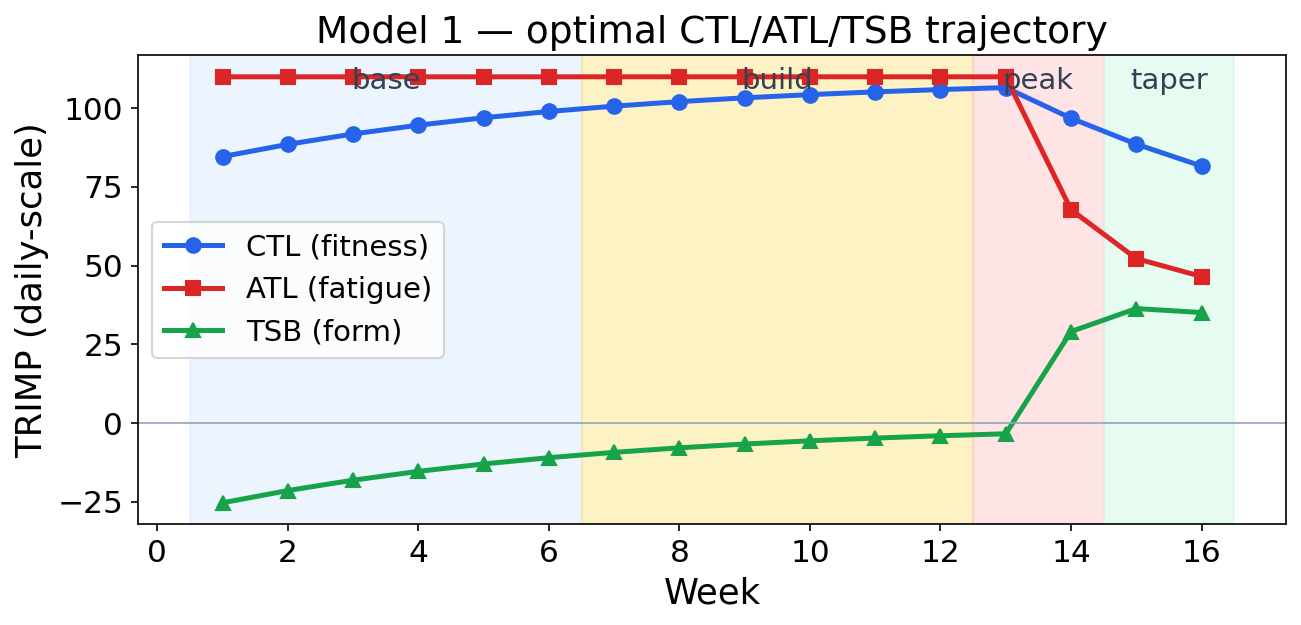
\includegraphics[width=.72\textwidth]{model1_trajectory.png}
\takeaway{Nobody told it to periodize. Week 14 tapers by choice.}
\end{frame}

\note{\gr Αυτό είναι το αγαπημένο μου αποτέλεσμα σε όλη την εργασία. Πουθενά στο
μοντέλο δεν γράφει «κάνε περιοδικότητα». Οι περιορισμοί είναι τοπικοί --- ένας
ρυθμός αύξησης, ένα ταβάνι, ένα κατώφλι --- και ο optimizer παράγει μόνος του
τον κλασικό μακρόκυκλο: κυλάει πάνω στο ταβάνι κόπωσης για δεκατρείς εβδομάδες,
ανεβάζοντας το CTL από 78 στο 107, και μετά κάνει taper.

Και προσέξτε την εβδομάδα 14. Μόνο οι εβδομάδες 15 και 16 είναι αναγκασμένες να
κάνουν taper. Η 14 κάνει taper επειδή το LP υπολογίζει ότι η κόπωση την ημέρα
του αγώνα κοστίζει περισσότερο απ' ό,τι αξίζει η φόρμα που θα αγόραζαν εκείνες
οι ώρες. Δηλαδή το μοντέλο ξαναβγάζει μόνο του προπονητική γνώση, από καθαρή
αριθμητική. Η φόρμα την ημέρα του αγώνα βγαίνει συν 35.}

\begin{frame}{Model 1 --- duality in action}
\begin{columns}
\column{.5\textwidth}
\centering
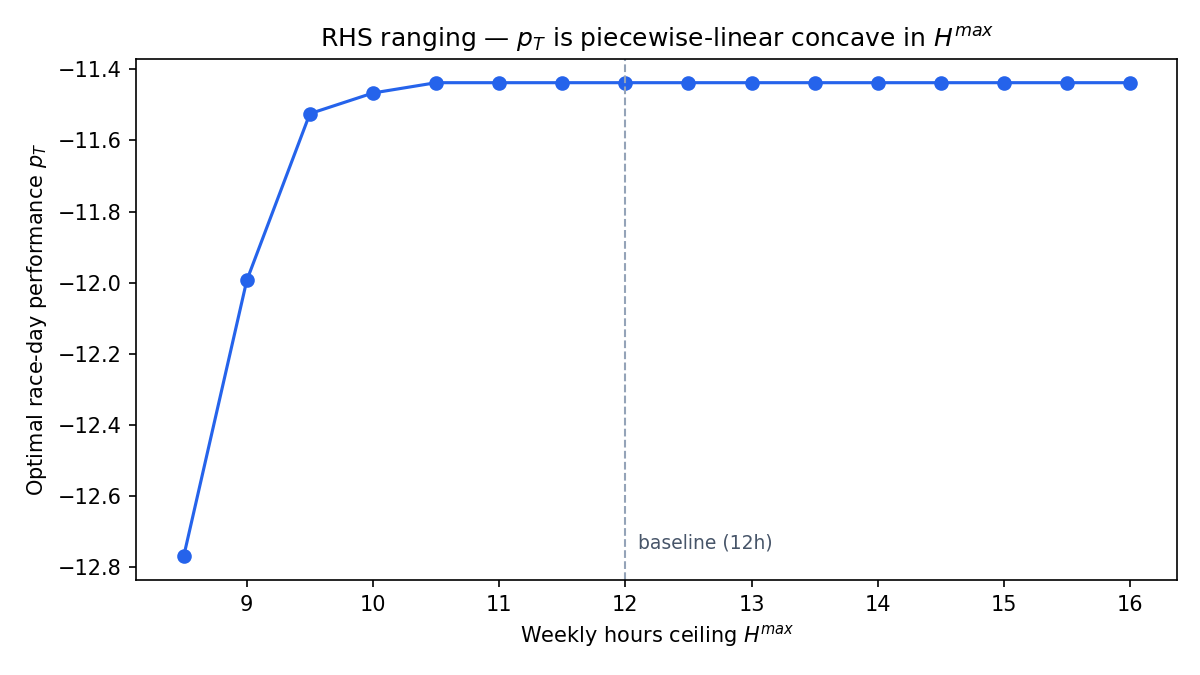
\includegraphics[width=\textwidth]{model1_rhs_ranging.png}
\column{.48\textwidth}
\textbf{RHS ranging:} the hours ceiling, 8--16 h
\begin{itemize}\itemsep6pt
  \item piecewise-linear, concave
  \item slopes $1.55 \to 0.94 \to 0.12 \to 0$
  \item flat above \textbf{10.5 h/week}
\end{itemize}
\vspace{10pt}
\begin{center}
\emph{Recovery capacity, not free time,\\ is what limits this athlete.}
\end{center}
\end{columns}
\end{frame}

\note{\gr Εδώ είναι η ανάλυση ευαισθησίας του μαθήματος, εφαρμοσμένη σε ένα
ερώτημα που με αφορά πραγματικά: αξίζει να ψάξω να βρω κι άλλες ώρες για
προπόνηση;

Μεταβάλλω το δεξί μέλος του περιορισμού των εβδομαδιαίων ωρών από 8 έως 16 και
σχεδιάζω τη βέλτιστη τιμή. Βγαίνει το σχήμα που προβλέπει η θεωρία: κατά
τμήματα γραμμική και κοίλη, επειδή κάθε σημείο καμπής είναι μια αλλαγή βάσης. Οι
κλίσεις είναι οι σκιώδεις τιμές: 1,55 μετά 0,94 μετά 0,12 και μετά μηδέν.

Η απάντηση βρίσκεται στις 10,5 ώρες. Από εκεί και πάνω η σκιώδης τιμή είναι
μηδέν: οι επιπλέον ώρες δεν αξίζουν τίποτα, γιατί το ταβάνι του ATL δεσμεύει
πριν προλάβει να δεσμεύσει το ταβάνι του χρόνου. Το στενό μου σημείο δεν είναι
το πρόγραμμά μου, είναι το πόσο γρήγορα ανακάμπτω.

Να αναφέρω και μία ακόμα δυϊκή τιμή: οι μεγαλύτερες σκιώδεις τιμές όλου του
μοντέλου είναι στους περιορισμούς ελάχιστης προπόνησης της εβδομάδας του αγώνα
--- μείον 12,9 ανά αναγκαστική ώρα τρεξίματος στην εβδομάδα 16. Το μοντέλο θέλει
απόλυτη ξεκούραση κι εγώ το υποχρεώνω να προπονηθεί.}

% ---------------------------------------------------------------- model 2
\begin{frame}{Model 2 --- race-calendar selection (0--1 MIP)}
\textbf{17 candidate races}, binary $x_i$
\[
\max \sum_i \underbrace{q_i(\alpha\,\text{pts}_i + \beta\,\text{strat}_i
+ \gamma\,\text{enj}_i + \varphi\,\text{fit}_i)}_{\text{weather-risk-adjusted value}} x_i
\]
\begin{itemize}\itemsep6pt
  \item \textbf{two knapsacks:} $\le 2500$ EUR, $\le 12$ vacation days
  \item \textbf{recovery spacing:} $x_i + x_j \le 1$; $\le 2$ races/month; $\ge 1$ A-race
  \item \textbf{readiness gate from Model 1:} projected CTL must reach the class
\end{itemize}
\end{frame}

\note{\gr Δεκαεπτά υποψήφιοι αγώνες --- ελληνικοί, ευρωπαϊκοί και δύο
υπερατλαντικοί --- ο καθένας με μία δυαδική μεταβλητή.

Η αξία κάθε αγώνα είναι τέσσερα σταθμισμένα συστατικά: βαθμοί παγκόσμιας
κατάταξης, στρατηγική σημασία, πόσο θα τον ευχαριστηθώ, και πόσο μου ταιριάζει η
διαδρομή. Το τελευταίο δεν είναι αίσθηση: υπολογίζεται από αντικειμενικά
δεδομένα διαδρομής, υψομετρική διαφορά ανά χιλιόμετρο σε σχέση με τη δική μου
προτίμηση σε επίπεδες διαδρομές. Και όλο αυτό πολλαπλασιάζεται με το q, έναν
συντελεστή καιρικού ρίσκου, ώστε ένας αγώνας με ιστορικό ακυρώσεων ή ακραίας
ζέστης να προεξοφλείται.

Τρεις οικογένειες περιορισμών. Δύο σακίδια --- χρήματα και ημέρες άδειας ---
που κάνουν το πρόβλημα δισδιάστατο knapsack. Ανά ζεύγος περιορισμοί αποθεραπείας,
μία, δύο ή τέσσερις εβδομάδες ανάλογα με την κατηγορία απόστασης, γραμμένοι με
τον τυπικό περιορισμό σύγκρουσης: x-i συν x-j το πολύ ένα. Και η πύλη
ετοιμότητας: το προβλεπόμενο CTL από το Μοντέλο 1 πρέπει να φτάνει την απαίτηση
της κατηγορίας --- εδώ ακριβώς μπαίνει φυσικά το Μοντέλο 1 μέσα στο Μοντέλο 2.
Αυτή η πύλη αποκλείει ένα 70.3 υψηλής αξίας στην αρχή της σεζόν: απλούστατα δεν
θα προλάβω να είμαι έτοιμος.}

\begin{frame}{Model 2 --- optimal season}
\centering
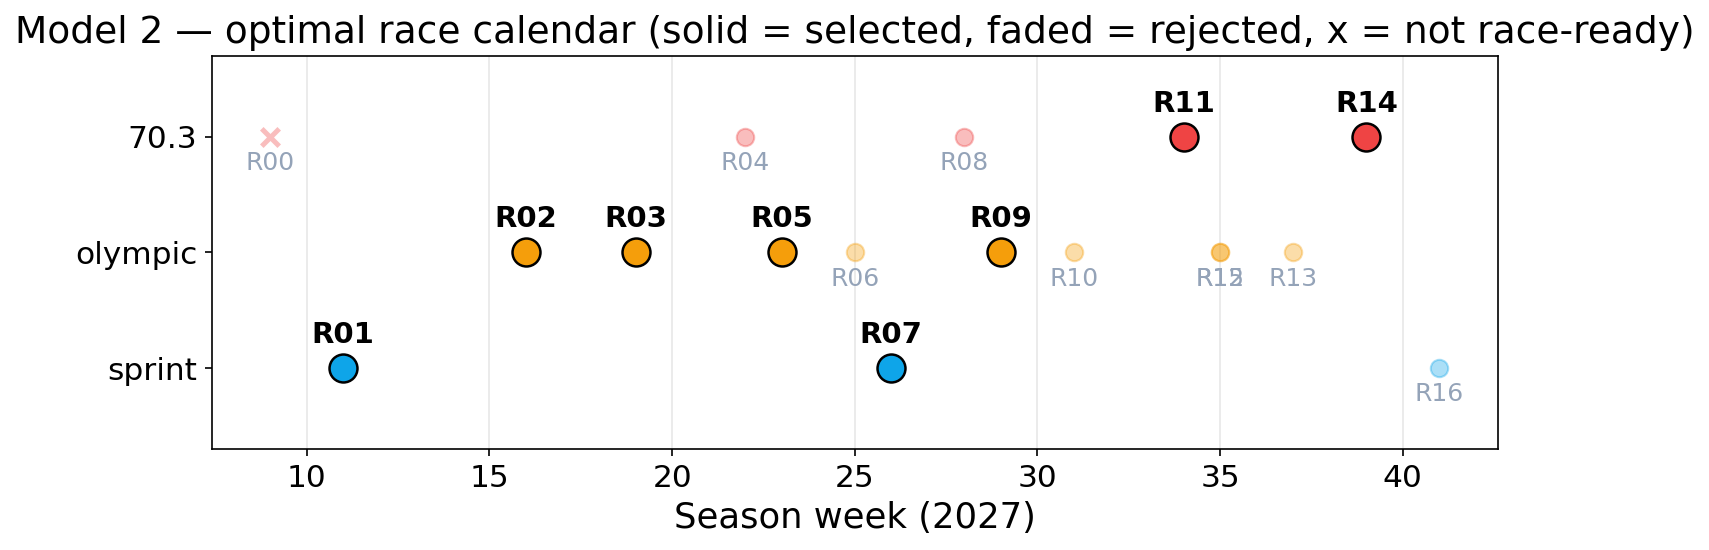
\includegraphics[width=.78\textwidth]{model2_calendar.png}
\takeaway{8 of 17 races $\cdot$ value 571.7 $\cdot$ 2250/2500 EUR $\cdot$ 11/12 days}
\end{frame}

\note{\gr Οκτώ αγώνες από τους δεκαεπτά, συνολική αξία 571,7. Ξοδεύει 2250 από τα
2500 ευρώ και 11 από τις 12 ημέρες άδειας --- άρα και τα δύο σακίδια είναι σχεδόν
γεμάτα, αλλά κανένα δεν δεσμεύει ακριβώς, κάτι που θα έχει σημασία σε δύο
διαφάνειες.

Η ενδιαφέρουσα απόφαση είναι το φθινόπωρο. Το Πανελλήνιο Πρωτάθλημα και το 70.3
της περιοχής μου είναι αρκετά κοντά ώστε ο περιορισμός αποθεραπείας να απαγορεύει
και τα δύο. Ο optimizer κρατάει το 70.3.

Τα «χι» είναι αγώνες για τους οποίους δεν είμαι αρκετά έτοιμος· οι ξεθωριασμένοι
κύκλοι είναι αγώνες που θα μπορούσε να πληρώσει αλλά επέλεξε να μην τους
αγοράσει.}

\begin{frame}{Model 2 --- why Branch \& Bound is needed}
\begin{columns}
\column{.52\textwidth}
\centering
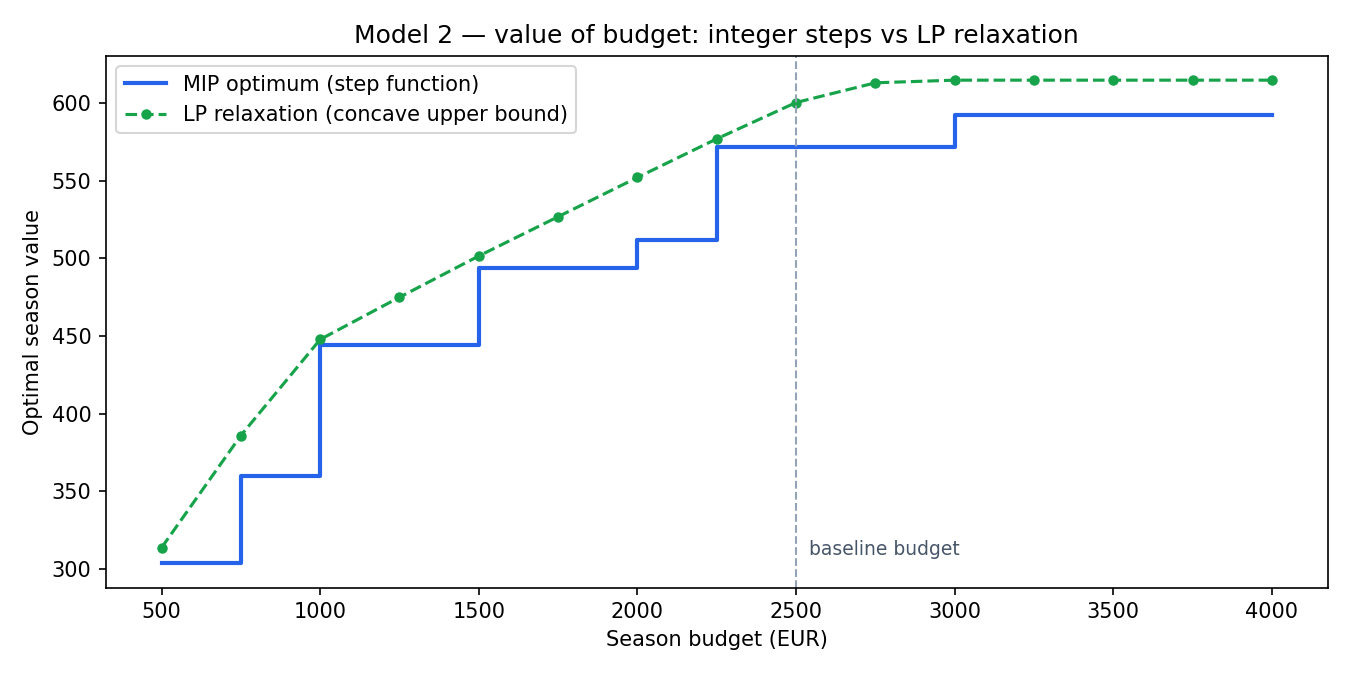
\includegraphics[width=\textwidth]{model2_budget_sweep.png}
\column{.46\textwidth}
\begin{itemize}\itemsep8pt
  \item LP $600.5$ vs.\ MIP $571.7$:\\ \textbf{integrality gap 5.0\%}
  \item 8 fractional variables; the champs/70.3 conflict splits \textbf{0.5/0.5}
  \item \textbf{clique cuts} (Bron--Kerbosch): $600.5 \to 591.0$,\\
        gap \textbf{5.04\% $\to$ 3.38\%}
\end{itemize}
\end{columns}
\end{frame}

\note{\gr Γιατί δεν λύνω απλώς τη γραμμική χαλάρωση και στρογγυλοποιώ; Επειδή η
χαλάρωση δίνει 600,5 έναντι πραγματικού βέλτιστου 571,7 --- κενό ακεραιότητας 5
τοις εκατό --- και οκτώ μεταβλητές βγαίνουν κλασματικές. Η σύγκρουση Πρωτάθλημα
εναντίον 70.3 που μόλις περιέγραψα σπάει ακριβώς μισό-μισό: η χαλάρωση παίρνει
μισό από κάθε αγώνα, που δεν σημαίνει τίποτα. Χρειάζεται Branch and Bound.

Το σχήμα είναι η αξία του χρήματος. Το βέλτιστο του MIP είναι κλιμακωτή
συνάρτηση --- οι αγώνες κοστίζουν όσο κοστίζουν, οπότε τα επιπλέον ευρώ δεν
κάνουν τίποτα μέχρι να φτάσουν να πληρώσουν άλλη μία συμμετοχή --- και βρίσκεται
κάτω από την κοίλη καμπύλη της χαλάρωσης. Πάνω από τα 3000 ευρώ τα σκαλοπάτια
σταματούν, γιατί ο δεσμευτικός πόρος αλλάζει από χρήματα σε ημέρες άδειας.

Για τα cutting planes: φτιάχνω τον γράφο συγκρούσεων των περιορισμών αποθεραπείας
και τρέχω Bron--Kerbosch για να βρω τις μέγιστες κλίκες του. Κάθε κλίκα μεγέθους
τρία ή παραπάνω δίνει μια έγκυρη ανισότητα, άθροισμα των x της κλίκας το πολύ
ένα, που κυριαρχεί των ανά ζεύγος περιορισμών. Τέσσερις τέτοιες τομές σφίγγουν τη
χαλάρωση από 600,5 σε 591, κλείνοντας το ένα τρίτο του κενού, και δεν αποκόπτουν
κανένα ακέραιο σημείο --- το βέλτιστο μένει αμετάβλητο.}

\begin{frame}{Model 2 --- the dual problem}
\[
\kappa_i y_\mathcal{B} + \delta_i y_\mathcal{D} + y_{\text{month}(i)}
+ \sum_{j} y_{ij} - [i \in A] y_A \;\ge\; v_i
\]
\begin{center}\small
\emph{a race enters only if its value covers the shadow cost of what it consumes}
\end{center}
\vspace{4pt}
\begin{center}\small
\begin{tabular}{llr}
\toprule
Dual & Meaning & Price\\
\midrule
$y_{13,14}$ & Champs vs.\ Costa Navarino conflict & \textbf{56.40}\\
$y_{06,07}$ & Hamburg vs.\ Thessaloniki conflict & 31.67\\
$y_\mathcal{B}$ & one extra euro & 0.094\\
$y_\mathcal{D}$ & one extra vacation day & $\approx 0$\\
\bottomrule
\end{tabular}
\end{center}
\takeaway{The scarce resource is calendar space --- not money.}
\end{frame}

\note{\gr Η γραμμική χαλάρωση είναι ήδη σε τυπική μορφή, max c-ανάστροφο-x υπό Ax
μικρότερο ή ίσο του b με x μη αρνητικό, οπότε το δυϊκό είναι το σχολικό: min
b-ανάστροφο-y με A-ανάστροφο-y μεγαλύτερο ή ίσο του c. Γράφοντας μία δυϊκή γραμμή
παίρνω την ανισότητα της διαφάνειας, και έχει καθαρή ανάγνωση: ένας αγώνας μπαίνει
στο ημερολόγιο μόνο αν η αξία του καλύπτει το σκιώδες κόστος όλων όσων καταναλώνει
--- budget, ημέρες άδειας, τη θέση του μήνα του, και κάθε σύγκρουση στην οποία
συμμετέχει.

Τώρα διαβάστε τις τιμές. Ένα ευρώ αξίζει 0,094. Μία ημέρα άδειας ουσιαστικά
μηδέν. Αλλά η σύγκρουση αποθεραπείας ανάμεσα στο Πρωτάθλημα και στην Costa
Navarino τιμολογείται στο 56,4 --- τρεις τάξεις μεγέθους πάνω από το ευρώ.

Άρα η διαίσθηση με την οποία ξεκίνησα ήταν λάθος. Υπέθετα ότι ο περιορισμός ήταν
τα χρήματα. Το δυϊκό λέει ότι ο σπάνιος πόρος είναι ο χώρος στο ημερολόγιο: οι
εβδομάδες αποθεραπείας μεταξύ αγώνων. Πρακτικά, το να διαπραγματευτώ ημερομηνίες
αξίζει πολύ περισσότερο από το να βρω χορηγία.}

\begin{frame}{Model 2 --- network-flow extension}
Drop the knapsacks and the monthly cap $\Rightarrow$ only recovery spacing remains:
\begin{center}
\textbf{feasible calendars $=$ paths in a DAG}
\end{center}
\vspace{6pt}
Three methods, identical answer $z = 639.4$:
\begin{enumerate}\itemsep4pt
  \item dynamic programming --- longest path in topological order
  \item \textbf{flow LP, continuous variables --- integral anyway}
  \item restricted 0--1 MIP
\end{enumerate}
\takeaway{Totally unimodular. The knapsacks are what break the structure.}
\end{frame}

\note{\gr Αυτή η διαφάνεια συνδέει την εργασία με το κομμάτι των δικτύων της ύλης.

Αν αφαιρέσω τα δύο σακίδια και το μηνιαίο πλαφόν, και κρατήσω μόνο την
αποθεραπεία, το πρόβλημα αλλάζει τελείως χαρακτήρα. Βάζω τους αγώνες ως κόμβους
σε σειρά εβδομάδας και τραβάω ακμή από τον i στον j όταν το κενό είναι
τουλάχιστον όσο η αποθεραπεία που απαιτεί ο i. Τότε ένα εφικτό ημερολόγιο είναι
ακριβώς μια διαδρομή σε αυτό το κατευθυνόμενο άκυκλο γράφημα, και το καλύτερο
ημερολόγιο είναι η μακρύτερη διαδρομή.

Το έλυσα με τρεις τρόπους και πήρα 639,4 και τις τρεις φορές. Ο μεσαίος είναι το
θεωρητικό σημείο: το έλυσα ως LP ροής με συνεχείς μεταβλητές, χωρίς κανέναν
περιορισμό ακεραιότητας, και η λύση βγήκε ακέραια από μόνη της. Αυτό είναι ολική
μονοπαραγοντικότητα --- ο πίνακας πρόσπτωσης κόμβων-ακμών είναι TU, άρα κάθε
βασική εφικτή λύση είναι ακέραια και κάθε βάση αντιστοιχεί σε ένα συνδετικό
δέντρο. Αυτή ακριβώς είναι η δομή που εκμεταλλεύεται ο Network Simplex. Δεκαοκτώ
κόμβοι, 136 ακμές.

Και αυτό λέει κάτι για το πλήρες μοντέλο: είναι οι περιορισμοί σακιδίου, το
budget και οι ημέρες άδειας, που καταστρέφουν τη δομή δικτύου και επιβάλλουν
Branch and Bound. Χωρίς αυτούς, δεν χρειάζεται καθόλου διακλάδωση.}

% ---------------------------------------------------------------- model 3
\begin{frame}{Model 3 --- race pacing (LP with linearization)}
\textbf{Variables} \quad minutes $t_{\ell z}$: 3 legs $\times$ 5 zones $= 15$
\vspace{4pt}

\textbf{Linearization} \quad within a zone, speed and energy rate are \emph{constants}
\[
\min \sum_{\ell,z} t_{\ell z} + T_1 + T_2
\quad \text{s.t.} \quad
\underbrace{\textstyle\sum_z s_{\ell z} t_{\ell z} \ge d_\ell}_{\text{distances}},\;
\underbrace{\textstyle\sum e_{\ell z} t_{\ell z} \le k_E \cdot \text{CTL}_T}_{\text{energy budget (Model 1)}},\;
\underbrace{\text{Z4+ caps}}_{\text{per leg}},\;
\underbrace{\varphi \cdot G}_{\text{bike} \to \text{run}}
\]
\vspace{-6pt}
\begin{center}\small
bike speed $\propto \phi(\gamma)\cdot(\text{power})^{1/3}$ \quad --- \quad
$\phi(\gamma)$ from the power balance, \textbf{derived, not fitted}
\end{center}
\end{frame}

\note{\gr Εδώ η φυσική είναι μη γραμμική: η σχέση ταχύτητας και ενεργειακού
κόστους είναι καμπύλη, όχι ευθεία. Το κόλπο είναι να διακριτοποιήσω την ένταση
στις πέντε προπονητικές ζώνες. Μέσα σε μια ζώνη, η ταχύτητα και ο ρυθμός
κατανάλωσης είναι σταθερές, άρα και η απόσταση και η ενέργεια γίνονται γραμμικές
ως προς τον χρόνο που ξοδεύω εκεί, και το πρόβλημα ξαναγίνεται LP. Δεκαπέντε
μεταβλητές. Αυτή είναι η κλασική κατά τμήματα γραμμική προσέγγιση του μαθήματος,
και οι ζώνες δεν είναι αυθαίρετες --- είναι οι ζώνες στις οποίες προπονούνται
πραγματικά οι αθλητές.

Δύο όροι αξίζουν κουβέντα. Η ταχύτητα στο ποδήλατο πάει με την κυβική ρίζα της
ισχύος, επειδή η αεροδυναμική αντίσταση πάει με την ταχύτητα στον κύβο --- αν
διπλασιάσεις την ισχύ σου δεν πλησιάζεις καν τον διπλασιασμό της ταχύτητας.

Και το φι του γάμμα είναι ο συντελεστής κλίσης της διαδρομής. Μοντελοποιώ μια
διαδρομή που ανεβαίνει γάμμα μέτρα ανά χιλιόμετρο ως μισή ανηφόρα και μισή
κατηφόρα με σταθερή ισχύ, και παίρνω τον αρμονικό μέσο των δύο ταχυτήτων. Η
αεροδυναμική σταθερά προκύπτει αντίστροφα από τη δική μου ταχύτητα σε επίπεδη
διαδρομή, οπότε τίποτα μέσα στο φι δεν είναι προσαρμοσμένο σε αποτέλεσμα αγώνα.
Αυτό θα έχει σημασία στην επικύρωση, τρεις διαφάνειες πιο κάτω.

Ο τελευταίος όρος είναι η σύζευξη που κάνει το πρόβλημα τρίαθλο και όχι τρεις
ξεχωριστούς αγώνες: κάθε κιλοτζάουλ σκληρής δουλειάς στο ποδήλατο μειώνει το πόσο
μακριά μπορώ μετά να τρέξω.}

\begin{frame}{Model 3 --- ``steady bike, hard run,'' derived}
\centering
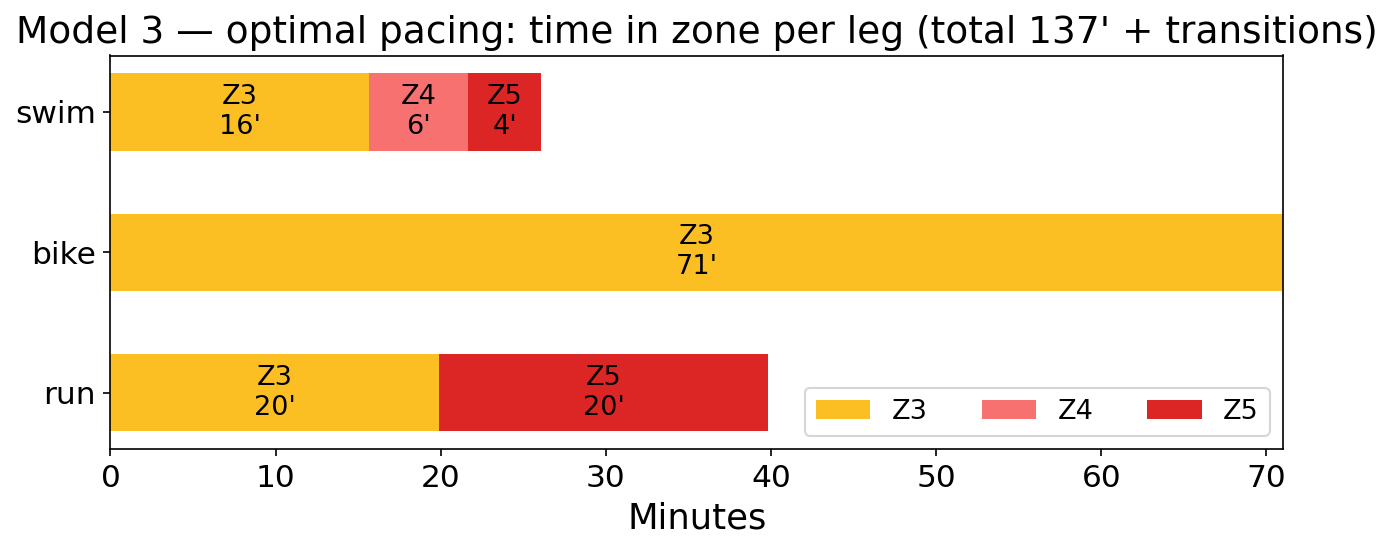
\includegraphics[width=.70\textwidth]{model3_pacing.png}
\takeaway{Bike entirely Z3. Energy budget exhausted \emph{exactly}: 9389 kJ.}
\end{frame}

\note{\gr Ολυμπιακή απόσταση σε 140,4 λεπτά, και το ενεργειακό budget εξαντλείται
ακριβώς --- 9389 κιλοτζάουλ διαθέσιμα, 9389 καταναλωμένα. Ο ενεργειακός
περιορισμός είναι δεσμευτικός, γι' αυτό και η δυϊκή του τιμή είναι το ενδιαφέρον
νούμερο της επόμενης διαφάνειας.

Η δομή της απάντησης είναι το προπονητικό κλισέ «σταθερό ποδήλατο, δυνατό
τρέξιμο», και το LP το βγάζει χωρίς να του το πει κανείς. Το ποδήλατο είναι
εξ ολοκλήρου στη ζώνη 3, τίποτα πιο σκληρό. Γιατί; Για δύο λόγους, και οι δύο
μέσα στο μοντέλο: η κυβική ρίζα σημαίνει ότι το σκληρό ποδήλατο αγοράζει ελάχιστη
ταχύτητα, και ο όρος σύζευξης σημαίνει ότι σου κοστίζει άμεσα απόσταση στο
τρέξιμο. Οπότε ο optimizer ξοδεύει την ένταση εκεί που η ένταση είναι φθηνή,
δηλαδή στο τρέξιμο.}

\begin{frame}{Model 3 --- what is a watt worth?}
\centering
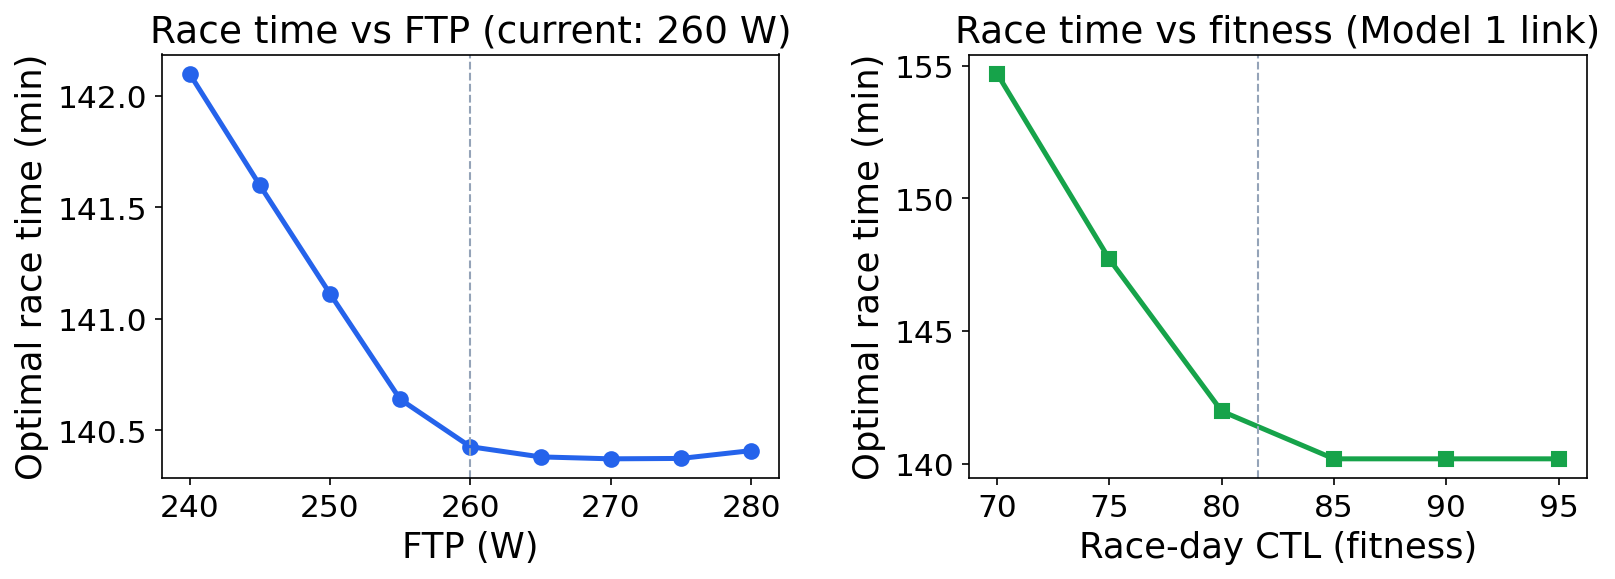
\includegraphics[width=.86\textwidth]{model3_sweeps.png}
\takeaway{$+1$ CTL $=$ 69--84 s. $+1$ W $\approx$ 6 s --- but only below 260 W.}
\end{frame}

\note{\gr Δύο σαρώσεις ευαισθησίας, και οι δύο απαντούν σε ερωτήματα που κάνει
ένας πραγματικός αθλητής.

Αριστερά: τι αξίζει ένα βατ; Κάτω από τα 260 βατ, κάθε επιπλέον βατ threshold
ισχύος αξίζει περίπου έξι δευτερόλεπτα. Πάνω από εκεί, η αξία καταρρέει στο μηδέν.
Αυτό δεν είναι σφάλμα --- είναι ο ενεργειακός περιορισμός. Με σταθερό απόθεμα
κιλοτζάουλ, δεν έχει νόημα να μπορείς να παράγεις περισσότερη ισχύ, γιατί δεν
μπορείς να την τροφοδοτήσεις. Το σκέλος του ποδηλάτου γίνεται ενεργειακά
περιορισμένο αντί για περιορισμένο από ισχύ.

Δεξιά: τι αξίζει μία μονάδα φόρμας; Εξήντα εννιά έως ογδόντα τέσσερα δευτερόλεπτα
ανά μονάδα CTL, και κρατάει μέχρι περίπου CTL 85.

Άρα τα δύο νούμερα μαζί δίνουν ξεκάθαρο προπονητικό συμπέρασμα: χτίσε αντοχή, όχι
μέγιστη ισχύ. Και αυτό βγήκε από σκιώδη τιμή, όχι από γνώμη. Η ίδια η δυϊκή τιμή
της ενέργειας, παρεμπιπτόντως, είναι 0,43 δευτερόλεπτα ανά κιλοτζάουλ.}

\begin{frame}{Model 3 --- validated against three real races}
\begin{center}\small
\begin{tabular}{llrrrrrr}
\toprule
& & \multicolumn{2}{c}{Swim} & \multicolumn{2}{c}{Bike} & \multicolumn{2}{c}{Run}\\
Race & CTL & mdl & act & mdl & act & mdl & act\\
\midrule
Spetsathlon '26 (sprint$^\ast$) & 64.9 & 12.9 & 13.2 & 47.3 & 50.9 & 18.7 & 17.7\\
Epidavros '25 (Olympic) & 55.6 & 27.2 & 25.8 & 88.8 & 91.5 & 38.9 & 42.0\\
70.3 Costa Navarino '25 & 71.4 & 33.3 & 32.9 & 184.6 & 180.3 & 86.4 & \textbf{115.2}\\
\bottomrule
\end{tabular}

{\scriptsize minutes $\cdot$ $^\ast$non-standard 25 km bike}
\end{center}
\vspace{4pt}
\begin{itemize}\itemsep5pt
  \item swim within 0.5 min every time
  \item binding constraint \textbf{switches with distance}: speed caps $\to$ energy
        $\to$ infeasible unfed
  \item the 70.3 run: my \textbf{29-minute} wall is the energy constraint, violated in real life
\end{itemize}
\end{frame}

\note{\gr Αυτό είναι το κομμάτι που δεν θα μπορούσα να κάνω με πλασματικά
δεδομένα. Βρήκα τις τρεις ημέρες αγώνα μέσα στο ακατέργαστο export --- είναι οι
μόνες τρεις μέρες που περιέχουν κολύμπι, ποδήλατο και τρέξιμο --- και πήρα την
κατάσταση φόρμας από την αλυσίδα επεξεργασίας, από την προηγούμενη μέρα. Τίποτα
εδώ δεν ρυθμίστηκε για να δείχνουν ωραία τα νούμερα.

Το κολύμπι πέφτει μέσα σε μισό λεπτό και τις τρεις φορές, που μου λέει ότι τα
μετρημένα κατώφλια είναι σωστά.

Η επιστημονικά ενδιαφέρουσα γραμμή είναι η μεσαία: το ποιος περιορισμός δεσμεύει
αλλάζει με την απόσταση του αγώνα. Στο sprint είναι τα πλαφόν ταχύτητας των
ζωνών --- με περιορίζει η τελική ταχύτητα, όχι το καύσιμο. Στην ολυμπιακή είναι η
ενέργεια. Στο 70.3 το μοντέλο βγαίνει εντελώς ανέφικτο με μόνο την αποθηκευμένη
ενέργεια· λύνεται μόνο αν το ταΐσεις. Και η πρόσληψη που χρειάζεται είναι περίπου
21 κιλοτζάουλ το λεπτό, που μεταφράζεται σε 75 γραμμάρια υδατανθράκων την ώρα ---
την τυπική οδηγία της αθλητικής διατροφής, ανακτημένη από ένα γραμμικό πρόγραμμα
που δεν την είχε ακούσει ποτέ.

Και τώρα η τίμια αποτυχία. Το μοντέλο προβλέπει 86 λεπτά για το τρέξιμο του 70.3·
εγώ έκανα 115. Αλλά δείτε τι συνέβη: μετά το δέκατο χιλιόμετρο πήγα από 4:53 ανά
χιλιόμετρο σε 5:52, με τον παλμό να πέφτει από 162 σε 145. Το να επιβραδύνεις ενώ
ο παλμός σου πέφτει δεν είναι κακή διαχείριση ρυθμού, είναι να σου τελειώνει το
καύσιμο. Άρα αυτά τα 29 λεπτά δεν είναι λάθος του μοντέλου --- είναι εγώ που
παραβίασα τον ενεργειακό περιορισμό στην πραγματικότητα. Το μοντέλο μου λέει πόσο
μου κόστισε.}

\begin{frame}{What the bike residual is made of}
\begin{center}\small
\begin{tabular}{lrrrrr}
\toprule
Bike leg & m/km & no gradient & $\phi(\gamma)$ & 2-param fit & actual\\
\midrule
Spetsathlon (24.4 km) & 15.2 & 43.3 & \textbf{47.3} & 55.0 & 50.9\\
Epidavros (38.7 km) & 15.5 & 78.9 & \textbf{88.8} & 87.7 & 91.5\\
Costa Navarino (88.5 km) & 9.1 & 177.5 & \textbf{184.6} & 180.0 & 180.3\\
\midrule
\multicolumn{2}{l}{total error} & 23.0 min & \textbf{10.6 min} & 8.2 min & \\
\multicolumn{2}{l}{parameters fitted here} & 0 & \textbf{0} & 2 & \\
\bottomrule
\end{tabular}
\end{center}
\vspace{6pt}
\begin{itemize}\itemsep5pt
  \item no gradient $\Rightarrow$ too fast on \textbf{every} course: a missing term, not noise
  \item $\phi(\gamma)$ from physics halves the error with \textbf{zero} fitted parameters
\end{itemize}
\end{frame}

\note{\gr Το ποδήλατο είναι το λιγότερο ακριβές σκέλος, οπότε θέλω να δείξω ότι
ξέρω γιατί, αντί να ελπίζω ότι δεν θα ρωτήσει κανείς.

Το ερώτημα: το υπόλοιπο του ποδηλάτου είναι απλώς θόρυβος, ή λείπει όρος από το
μοντέλο; Δύο στοιχεία λένε ότι λείπει όρος. Πρώτον το μέγεθος --- 23 λεπτά σε
τρεις αγώνες. Δεύτερον, και πιο αποκαλυπτικό, το πρόσημο: αν προσποιηθώ ότι κάθε
διαδρομή είναι επίπεδη, βγαίνω γρηγορότερος και στις τρεις. Ο θόρυβος δεν έχει
πρόσημο.

Ο όρος που λείπει είναι η κλίση, και επίτηδες δεν την κόλλησα εκ των υστέρων.
Ανήκει στη διατύπωση, οπότε το φι του γάμμα είναι μέρος του μοντέλου, παραγόμενο
από το ισοζύγιο ισχύος του ποδηλάτου, με μηδέν παραμέτρους προσαρμοσμένες σε
αυτούς τους αγώνες. Αυτό είναι γνήσιο out-of-sample τεστ και υποδιπλασιάζει το
σφάλμα στα 10,6 λεπτά, με τα υπόλοιπα να πέφτουν πλέον και από τις δύο πλευρές
του μηδενός.

Η τελευταία στήλη είναι ο έλεγχός μου. Προσάρμοσα και μια εμπειρική διόρθωση δύο
παραμέτρων κατευθείαν πάνω σε αυτούς τους τρεις αγώνες --- που είναι ζαβολιά, και
αποτελεί άνω φράγμα του πόσο καλή θα μπορούσε να φανεί οποιαδήποτε τέτοια
διόρθωση. Κερδίζει μόλις 2,4 λεπτά παραπάνω. Άρα η κλίση εξηγεί ουσιαστικά όλο το
ανακτήσιμο σφάλμα, και η παραγόμενη εκδοχή το παίρνει σχεδόν όλο δωρεάν.

Και η μικρή μεροληψία που απομένει εξηγείται κι αυτή: το φι υποθέτει ότι κρατάω
threshold ισχύ στις κατηφόρες, που δεν το κάνει κανείς, οπότε μένω ελαφρώς
αισιόδοξος στις δύο ανηφορικές διαδρομές.}

% ---------------------------------------------------------------- playing with the model
\begin{frame}{Sensitivity across sizes and parameters}
\begin{columns}
\column{.52\textwidth}
\centering
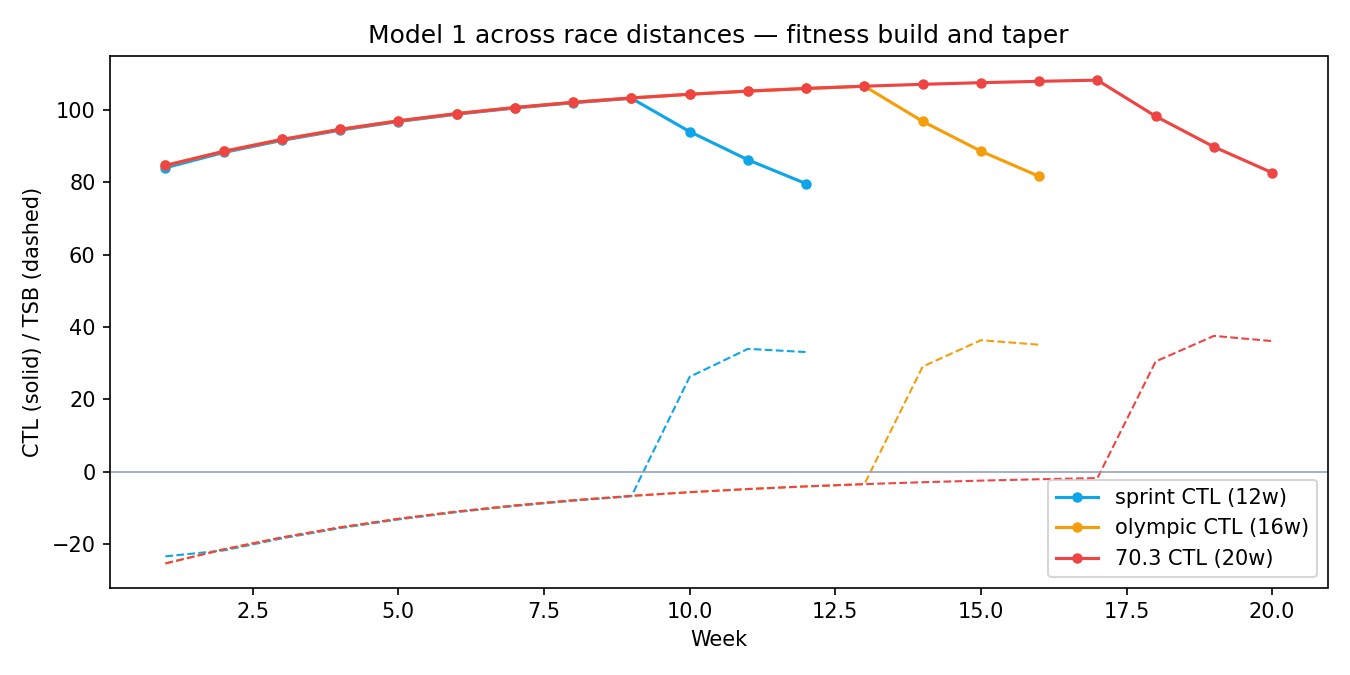
\includegraphics[width=\textwidth]{model1_distance_scenarios.png}
\column{.46\textwidth}
\begin{itemize}\itemsep10pt
  \item \textbf{Sizes:} 12/16/20 weeks, 144--240 vars --- structure invariant
  \item \textbf{$k_2 \in [1,3]$:} race-day TSB stays $35 \pm 2$
  \item \textbf{Cost ranging:} plan invariant for $k_1 \in [0.68, 1.56]$,
        $k_2 \in [1.29, 2.95]$
  \item \textbf{Solve times:} all $< 10$ ms
\end{itemize}
\end{columns}
\end{frame}

\note{\gr Η εκφώνηση ζητάει να «παίξουμε» με το μοντέλο, οπότε: τρία είδη
διαταραχής.

Μέγεθος. Ξανάτρεξα τον μακρόκυκλο σε 12, 16 και 20 εβδομάδες --- από 144 μέχρι
240 μεταβλητές. Οι μεγαλύτεροι ορίζοντες βοηθούν, η αντικειμενική πάει από μείον
13,5 σε μείον 10,4, με φθίνουσες αποδόσεις, και η δομή χτίσιμο-και-μετά-taper
είναι πανομοιότυπη και στις τρεις. Δηλαδή η ποιοτική απάντηση δεν εξαρτάται από
τον ορίζοντα που έτυχε να διαλέξω.

Βαθμονόμηση της αντικειμενικής. Το k2 είναι η παράμετρος για την οποία είμαι πιο
ανασφαλής, οπότε το σάρωσα από 1 έως 3: η φόρμα την ημέρα του αγώνα μετακινείται
ελάχιστα, 35 συν πλην 2. Το βάθος του taper το καθορίζουν οι περιορισμοί --- τα
ελάχιστα της εβδομάδας αγώνα --- όχι η αντικειμενική, κάτι που με καθησυχάζει
επειδή τους περιορισμούς τους έχω μετρήσει.

Και τυπικό cost ranging, κατευθείαν από την ύλη: η βέλτιστη βάση επιβιώνει για k1
οπουδήποτε από 0,68 έως 1,56 και k2 από 1,29 έως 2,95. Τα δύο λιγότερο μετρήσιμα
νούμερα του μοντέλου μπορούν να μεταβληθούν κατά παράγοντα δύο χωρίς να αλλάξει
ούτε μία μεταβλητή.

Όλα λύνονται σε λιγότερο από δέκα χιλιοστά του δευτερολέπτου, οπότε τίποτα από
αυτά δεν μου κόστισε.}

\begin{frame}{Integrating the pipeline: coherence \& fixed point}
\textbf{Do the three objectives agree?}
\begin{itemize}\itemsep5pt
  \item $E = k_E\text{CTL}$ ignores fatigue $\Rightarrow$ four different plans,
        \textbf{same 140.2 min}
  \item $E = E_0 + k_E(\text{CTL}_T - \lambda\,\text{ATL}_T)$ is affine in $p_T$
        \textbf{iff} $\lambda = k_2/k_1$
  \item $E > 0$ needs $\lambda < 1.75$, so $k_2 = 2$ is \emph{incoherent};
        cost ranging licenses $\lambda = 1.5$ --- \textbf{changing no variable}
\end{itemize}
\vspace{6pt}
\textbf{Which model comes first?} Iterate.
\begin{center}\small
\begin{tabular}{clrlr}
\toprule
Iter. & Macrocycle & Weeks & Selected A-race & Outcome\\
\midrule
1 & olympic & 16 & R14 Costa Navarino (70.3) & re-plan as 70.3\\
2 & 70.3 & 20 & R14 Costa Navarino (70.3) & \textbf{fixed point}\\
\bottomrule
\end{tabular}
\end{center}
\end{frame}

\note{\gr Δύο προβλήματα ολοκλήρωσης, που τα θεωρώ το πιο ενδιαφέρον κομμάτι της
εργασίας, επειδή και τα δύο ανακαλύφθηκαν με έλεγχο και όχι με υπόθεση.

Πρώτον, η συνέπεια. Το Μοντέλο 1 μεγιστοποιεί έναν δείκτη απόδοσης· το Μοντέλο 3
ελαχιστοποιεί χρόνο αγώνα. Συμφωνούν; Το δοκίμασα: παρήγαγα τέσσερα αρκετά
διαφορετικά προπονητικά πλάνα και τα έδωσα στο Μοντέλο 3, και τα τέσσερα έδωσαν
τα ίδια 140,2 λεπτά. Το Μοντέλο 3 ήταν τυφλό στην προπόνηση --- επειδή το
ενεργειακό budget ήταν k-E επί CTL, που αγνοεί τελείως την κόπωση. Μπορούσες να
κάνεις taper ή να μην κάνεις και ο αγώνας έβγαινε ίδιος. Αυτό είναι σπασμένη
αλυσίδα.

Η διόρθωση είναι ένα μικρό θεώρημα. Κάνε το budget να εξαρτάται από τη φόρμα:
E-μηδέν συν k-E επί CTL μείον λάμδα επί ATL. Τότε το budget είναι γνησίως αύξουσα
αφινική συνάρτηση της αντικειμενικής του Μοντέλου 1 ακριβώς όταν το λάμδα ισούται
με k2 προς k1 --- και σε αυτή την περίπτωση η μεγιστοποίηση της απόδοσης είναι
αποδεδειγμένα το ίδιο με την ελαχιστοποίηση του χρόνου. Τα μοντέλα
ευθυγραμμίζονται εξ ορισμού, όχι στην τύχη.

Υπάρχει όμως μια παγίδα, και είναι ωραία. Το budget πρέπει να μένει θετικό, που
απαιτεί λάμδα μικρότερο από CTL προς ATL, δηλαδή 1,75. Το k2 που είχα υποθέσει
ίσο με 2 δίνει λάμδα 2 --- ασυνεπές. Άρα το θεώρημα δεν ευθυγραμμίζει απλώς τα
μοντέλα, απορρίπτει μια παράμετρο που είχα διαλέξει. Και εδώ αποδίδει το cost
ranging της προηγούμενης διαφάνειας: λέει ότι το k2 οπουδήποτε από 1,29 έως 2,95
αφήνει το πλάνο αμετάβλητο. Οπότε βάζω λάμδα 1,5, η αλυσίδα γίνεται συνεπής, και
δεν κουνιέται ούτε μία από τις 144 μεταβλητές.

Δεύτερον, η κυκλικότητα. Ο αγώνας-στόχος ορίζει το μήκος του μακρόκυκλου για το
Μοντέλο 1, αλλά το Μοντέλο 1 τροφοδοτεί την πύλη ετοιμότητας του Μοντέλου 2 που
επιλέγει τον αγώνα-στόχο. Αντί να υποθέσω σειρά, έκανα επανάληψη μέχρι σταθερό
σημείο --- δύο επαναλήψεις. Και η επανάληψη βρήκε πραγματικό λάθος: είχα υποθέσει
16 εβδομάδες για ολυμπιακή, αλλά ο αγώνας-στόχος που επιλέγει το ημερολόγιο είναι
70.3, που θέλει 20 εβδομάδες. Αν είχα υποθέσει σειρά, αυτό θα έμενε κρυφό.}

% ---------------------------------------------------------------- payoff
\begin{frame}{What the models actually recommend}
\begin{itemize}\itemsep9pt
  \item \textbf{Train more, much easier.} 6.6 h/wk at 37\% hard
        $\rightarrow$ 9.0 h/wk at \textbf{15\%}
  \item \textbf{More hours are worthless} above 10.5 h/wk --- recovery is what binds
  \item \textbf{Build endurance, not watts.} $+1$ CTL $=$ 69--84 s; $+1$ W $\approx 0$ above 260 W
  \item \textbf{Ride Z3, run hard, fuel 75 g/h.} The 70.3 positive split cost 29 min
  \item \textbf{Protect the calendar, not the budget.} Conflict dual 56.4 vs.\ 0.094/EUR
\end{itemize}
\end{frame}

\note{\gr Αν πάρω στα σοβαρά τη δική μου εργασία, να τι αλλάζει από τη Δευτέρα.

Η πρώτη γραμμή είναι αυτή που πονάει. Αυτή τη στιγμή προπονούμαι 6,6 ώρες την
εβδομάδα με το 37 τοις εκατό σκληρό. Το μοντέλο λέει 9 ώρες με 15 τοις εκατό
σκληρό. Είμαι αντι-πολωμένος --- προπονούμαι πολύ λίγο και πολύ δυνατά. Είναι η
μία αλλαγή με τη μεγαλύτερη απόδοση, και δεν θα την πίστευα χωρίς τις σκιώδεις
τιμές.

Δεύτερον, πρέπει να σταματήσω να ψάχνω κι άλλες ώρες προπόνησης πάνω από τις
δέκα μισή· αξίζουν κυριολεκτικά μηδέν. Ο δεσμευτικός πόρος είναι η ικανότητα
αποκατάστασης.

Τρίτον, από τη σάρωση των βατ: δουλειά αντοχής, όχι threshold ισχύς.

Τέταρτον, εκτέλεση αγώνα: ποδήλατο στη ζώνη 3, κράτα το για το τρέξιμο, σταθερός
ρυθμός, και 75 γραμμάρια υδατανθράκων την ώρα. Το θετικό σπλιτ μου στο 70.3
κόστισε 29 λεπτά.

Πέμπτον, διαπραγματεύσου ημερομηνίες αντί να κυνηγάς χρήματα --- 56,4 έναντι
0,094.

Και μία διόρθωση σχεδιασμού που την αποκάλυψε μόνο η επανάληψη σταθερού σημείου:
παράλειψε το Ντουμπάι στην αρχή της σεζόν γιατί δεν θα προλάβω να είμαι έτοιμος,
και αν ο αγώνας-στόχος είναι 70.3, χτίσε 20 εβδομάδες, όχι 16.}

\begin{frame}{Conclusions}
\begin{itemize}\itemsep10pt
  \item Three coupled models on \textbf{real personal data}
  \item Spanning the syllabus: LP \& Simplex, duality \& sensitivity,
        IP \& Branch \& Bound, network flows \& total unimodularity
  \item The optimizer \textbf{re-derives coaching wisdom} --- periodization,
        polarization, ``steady bike, hard run''
  \item Duals name the real bottlenecks: \emph{recovery}, \emph{calendar space},
        \emph{endurance}
  \item Reproducible: \texttt{python -m src.run\_all}, 60 tests
\end{itemize}
\vspace{6pt}
\begin{center}
{\footnotesize\url{https://github.com/manos1503/triathlon-optimization}}

\vspace{6pt}
\Large Thank you --- questions?
\end{center}
\end{frame}

\note{\gr Κλείνοντας. Τρία συζευγμένα μοντέλα, χτισμένα πάνω σε πραγματικά
προσωπικά δεδομένα και όχι σε σχολικό παράδειγμα, και μαζί καλύπτουν ουσιαστικά
όλη την ύλη: LP και Simplex, δυϊκότητα και ανάλυση ευαισθησίας, ακέραιο
προγραμματισμό με Branch and Bound και τομές, και δίκτυα ροής με ολική
μονοπαραγοντικότητα.

Δύο πράγματα που δεν τα περίμενα όταν ξεκίνησα. Ο optimizer ξαναβγάζει
προπονητική γνώση που δεν του την είπε κανείς --- περιοδικότητα, πολωμένη ένταση,
σταθερό ποδήλατο και δυνατό τρέξιμο. Και οι δυϊκές τιμές διέψευσαν συστηματικά τη
διαίσθησή μου για το τι με περιορίζει: όχι ο χρόνος, όχι τα χρήματα, αλλά η
ικανότητα αποκατάστασης, ο χώρος στο ημερολόγιο, και η αντοχή.

Όλα τρέχουν με μία εντολή και καλύπτονται από 60 tests. Σας ευχαριστώ --- είμαι
στη διάθεσή σας για ερωτήσεις.}

% ---------------------------------------------------------------- backup
\appendix
\begin{frame}{Backup: limitations}
\begin{itemize}\itemsep8pt
  \item \textbf{Weekly} time step for the Banister dynamics
  \item \textbf{Sequential} pipeline, not joint optimization
  \item \textbf{Constructed parameters} in Models 2--3 (race values, zone speeds, $k_E$)
  \item The LP's $+35$ TSB over-taper --- traced to race-week minimums
\end{itemize}
\end{frame}

\note{\gr Ημερήσια ανάλυση θα μετακινούσε τις σταθερές εξομάλυνσης αλλά όχι τη
δομή. Η από κοινού βελτιστοποίηση προπόνησης και ημερολογίου είναι φυσική και
αρκετά μεγαλύτερη επέκταση MIP --- αυτή είναι η προφανής συνέχεια. Οι
κατασκευασμένες παράμετροι είναι τεκμηριωμένες ως παραδοχές, και η ανάλυση
ευαισθησίας υπάρχει ακριβώς για να δείξει ποια συμπεράσματα επιβιώνουν όταν τις
διαταράξω. Και το υπερβολικό taper είναι τεχνούργημα περιορισμού, όχι εννοιολογικό
ελάττωμα του μοντέλου.}

\begin{frame}{Backup: alternative optima \& heuristic benchmark}
\textbf{Alternative optima:} fix $p_T = p^\ast$, re-solve min/max total hours
\begin{center}
same performance with \textbf{124.2 h} or \textbf{162.3 h} of season training
\end{center}
\vspace{8pt}
\textbf{vs.\ a standard coaching heuristic:}
\begin{itemize}\itemsep5pt
  \item violates the fatigue ceiling in \textbf{13 of 16 weeks}
  \item $p_T = -69.5$ vs.\ optimal $-11.4$
  \item but its race-day TSB $+21$ is inside the coaching band; the LP's $+35$ is not
\end{itemize}
\end{frame}

\note{\gr Ο εκφυλισμός γίνεται ορατός: καθηλώνω την αντικειμενική στη βέλτιστη
τιμή της και μετά ελαχιστοποιώ και μεγιστοποιώ τις συνολικές ώρες προπόνησης υπό
αυτόν τον περιορισμό. Και τα δύο είναι βέλτιστα πλάνα, και διαφέρουν κατά 38 ώρες
προπόνησης μέσα στη σεζόν. Αυτό είναι πραγματικό κενό αποδοτικότητας που η
αντικειμενική από μόνη της δεν το βλέπει.

Ο ευρετικός κανόνας είναι αυτό που θα έγραφε ένας λογικός προπονητής --- γέμισε
τις διαθέσιμες ώρες, 20/45/35 στα αθλήματα, 80/15/5 στις εντάσεις. Σπάει το ταβάνι
κόπωσης σε 13 από τις 16 εβδομάδες, που είναι χρόνια υπερπροπόνηση, και βαθμολογεί
πολύ χειρότερα. Δίκαια όμως, φέρνει τη φόρμα της ημέρας του αγώνα μέσα στην
αποδεκτή προπονητική ζώνη ενώ το δικό μου LP όχι --- που είναι ακριβώς το ερώτημα
ευαισθησίας του k2 από πριν.}

\end{document}
